\documentclass[final]{nip} %%use nip class

%% to add options: phd, ms, bs, applied
\usepackage{fancyhdr}
\fancyhf{}
\rhead{\textbf{\nouppercase{\rightmark}}}
\cfoot{\thepage}

%%packages to be used.
\usepackage[square,numbers,sort&compress]{natbib}
   %% square-bracketed, numbered, sorted, and compressed citations

\usepackage{verbatim} %% for \verbatiminput
\usepackage{graphicx} %% for the graphics environment
\usepackage[centertags]{amsmath}
\usepackage{amsfonts}
\usepackage{amssymb}
\usepackage{amsthm}
\usepackage{mathtools}
\usepackage{newlfont}
\usepackage{enumitem}

% todo package: TO BE REMOVED IN THE FINAL DRAFT
\usepackage[colorinlistoftodos,prependcaption,textsize=footnotesize]{todonotes}

%for figures
\usepackage{caption}
\usepackage{subcaption}

%for table
\usepackage[]{array}
\newcolumntype{P}[1]{>{\centering\arraybackslash}p{#1}}

%for python codes
\usepackage{color}
\usepackage{listings}
\usepackage{setspace}
\definecolor{Code}{rgb}{0,0,0}
\definecolor{Decorators}{rgb}{0.5,0.5,0.5}
\definecolor{Numbers}{rgb}{0.5,0,0}
\definecolor{MatchingBrackets}{rgb}{0.25,0.5,0.5}
\definecolor{Keywords}{rgb}{0,0,1}
\definecolor{self}{rgb}{0,0,0}
\definecolor{Strings}{rgb}{0,0.63,0}
\definecolor{Comments}{rgb}{0,0.63,1}
\definecolor{Backquotes}{rgb}{0,0,0}
\definecolor{Classname}{rgb}{0,0,0}
\definecolor{FunctionName}{rgb}{0,0,0}
\definecolor{Operators}{rgb}{0,0,0}
\definecolor{Background}{rgb}{0.98,0.98,0.98}
\lstdefinelanguage{Python}{
numbers=left,
numberstyle=\footnotesize,
numbersep=1em,
xleftmargin=1em,
framextopmargin=2em,
framexbottommargin=2em,
breaklines=true,
showspaces=false,
showtabs=false,
showstringspaces=false,
frame=l,
tabsize=4,
% Basic
basicstyle=\ttfamily\small\setstretch{1},
backgroundcolor=\color{Background},
% Comments
commentstyle=\color{Comments}\slshape,
% Strings
stringstyle=\color{Strings},
comment=[l]{\#},
morecomment=[s][\color{Strings}]{"}{"},
morecomment=[s][\color{Strings}]{'}{'},
% keywords
morekeywords={import,from,class,def,for,while,if,is,in,elif,else,not,and,or,print,break,continue,return,True,False,None,access,as,,del,except,exec,finally,global,import,lambda,pass,print,raise,try,assert},
keywordstyle={\color{Keywords}\bfseries},
% additional keywords
morekeywords={[2]@invariant,pylab,numpy,np,scipy},
keywordstyle={[2]\color{Decorators}\slshape},
emph={self},
emphstyle={\color{self}\slshape},
%
}

\lstdefinelanguage{xml}{
numbers=left,
numberstyle=\footnotesize,
numbersep=1em,
xleftmargin=1em,
framextopmargin=2em,
framexbottommargin=2em,
breaklines=true,
showspaces=false,
showtabs=false,
showstringspaces=false,
frame=l,
tabsize=4,
% Basic
basicstyle=\ttfamily\small\setstretch{1},
backgroundcolor=\color{Background},
%
}

% %% Header section
% \title{Ground state correlations and entanglement in an extended Hubbard model with Ising-like interaction}
%% Header section
\title{Reduction Formulas of the Kampé de Fériet Function Arising from the Method of Finite-part Integration}
%%required
\author{Lloyd L. Villanueva} %% required
\email{llvillanueva@up.edu.ph}%% appears only when draft version use \draft option.
\adviser{Eric A. Galapon}{Ph.D.}%% required
\reader{Francis Norman C. Paraan}{Ph.D.}%% required
% \secondReader{}{Ph.D.}%% optional if with coadviser
%\coadviser{Another A. Adviser}{Ph.D.}%% replace "\coadviser" with "\secondReader" if no co-adviser
\director{Wilson O. Garcia}{Ph.D.}%% required
\dean{Giovanni A. Tapang}{Ph.D.} %%required
\gradyear{2021} \gradmonth{July} %%graduation month and year
\defenseDate{June 2021}

%% Preliminary pages' contents input here..
\acknowledgments{ I would like to dedicate this work and take this opportunity to express my great appreciation and deep gratitude to the people and institutions who have helped and supported me along the way.
\\*

To my adviser, Dr. Eric A. Galapon, for his infinite patience, for his encouragement and guidance leading up to the accomplishment of this work. He's still the master of infinities.
\\*

To my thesis reader Dr. Francis Norman C. Paraan, and to my examiners Dr. Johnrob Y. Bantang and Dr. Marvin M. Flores, for the constructive criticism on how to improve this work. 
\\*

To the Office of the Chancellor of the University of the Philippines Diliman, through the Office of the Vice Chancellor for Research and Development, for funding this work through the Outright Research Grant Project No. 191915 ORG.
\\*

To the National Institute of Physics and University of the Philippines, for giving me a high-quality education and molding me into the person I am today. Lagi't lagi Para sa Bayan. 
\\*

To my colleagues at the Theoretical Physics Group, especially to the QuantMath subgroup for companionship and constant encouragement.
\\*

To my highschool and UP Manila and Diliman friends who still continue to support and encourage me even though we do not see each other more often. 
\\*

To my co-instructors, especially to Batch 2019 and socials people, for all the help and making everything bearable. 
\\*

To my badminton buddies, for the active and healthy activities in this pandemic.
\\*



To my physics batchmate, especially to my physics buddies JJ, Angelo, and Theo, for the support and push to finish this degree and this work.
\\*

To my solid team teach and classmate since UP Manila days, Ser Ralph Farrales, for helping me in both teaching and acads stuff.
\\*

To my favorite math prof, Dr. Mia Mojica, for the continuous support and believing in my skills.
\\*

To Leonarc Michelle Santos, for being my solid physics teammate since high school.
\\*

To Ma. Paula Rafaella M. Ortiz and to her family, for helping me in everything. Without them, I will not be here in UP Diliman.  
\\*

To Moira Isobel Christine Sapitula, for being a genuine and wonderful person.
\\*

To my futsal and ultimate friends, especially to Carl, Micah, Kenneth, Jonah, Gabriel, Adrianne, Cedie, Anel, Ivy, Louie, etc. for the chill online/in-person activities.
\\*

To my college bestfriend, Charlyn O. Valdeavilla, for always listening to me whatever it is. To her family, Daryl, Faye, Dong, Arlyn, for the trust, kindness, and always being there to help. 
\\*

And most especially to my parents and siblings as my unlimited source of motivation to continue and for their endless support. 


 } %% optional, see acknowledgment.tex for sample content.
\abstract{ %Finite-part integration is a method of evaluating well-defined convergent integrals by means of the finite-part of divergent integrals. The method is known to exactly evaluate the Stieltjes transform $S_{\lambda} [f] = \int_0^\infty f(x)/(\omega + x)^{\lambda} \, \mathrm{d}x$ with the assumption that the complex extension of the function $f(x)$ is entire. The recent development of the method is the extension of its applicability to the Stieltjes transform of functions $f(x)$ with competing singularities in its complex extension. Also, the presence of singularities was found to impose a restriction to the radius of convergence of the infinite series of finite-part integrals. This infinite series of the finite-part integrals is evaluated to be the hypergeometric-type series containing digamma function as a factor in the case of pole singularity. Thus, the study of this series is necessary to lift this restriction. In this thesis, the convergence and analyticity of the generalized form of the mentioned series will be established. Then, the relation of this series to the Kampé de Fériet function will be derived. Furthermore, the obtained relation will be exploited, together with the results in the method of finite-part integration, to generate reduction formulas of the Kampé de Fériet function.
Finite-part integration is a method of evaluating well-defined convergent integrals by means of the finite-part of divergent integrals. The method is known to exactly evaluate the Stieltjes transform $S_{\lambda} [f] = \int_0^\infty f(x)/(\omega + x)^{\lambda} \, \mathrm{d}x$ with the assumption that the complex extension of the function $f(x)$ is entire. The recent development of the method is the extension of its applicability to the Stieltjes transform of functions $f(x)$ with competing singularities in its complex extension. Also, the presence of singularities was found to impose a restriction to the radius of convergence of the infinite series of finite-part integrals. In the case of pole singularity, the infinite series of the finite-part integrals takes the form of the hypergeometric-type series containing digamma function as a factor when evaluated. Thus, in order to lift the restriction, the study of the mentioned series is necessary. In this thesis, the convergence and analyticity of the generalized form of the mentioned series will be established. Then, the relation of this series to the Kampé de Fériet function will be derived. Furthermore, the obtained relation will be exploited, together with the results in the method of finite-part integration, to generate reduction formulas of the Kampé de Fériet function.

\noindent PACS: 02.30.Uu (Integral transforms); 02.30.Gp (Special functions); 02.30.Cj (Measure and integration) } %% see abstract.tex
\pacs{}

%\acronym{\newlist{abbrv}{itemize}{1}
\setlist[abbrv,1]{label=,labelwidth=2in,align=parleft,itemsep=0.2\baselineskip,leftmargin=!}


\begin{abbrv}
\item[$\Gamma(z)$]      Gamma Function
\item[$\Gamma(z,x)$]    Incomplete Gamma Function
\item[$\mathrm{Ei}(x)$] Exponential Integral Function          
\item[$\psi(z)$]        Digamma Function
\item[${}_2F_{1}$]      Gauss Hypergeometric Function
\item[${}_pF_{q}$]      Generalized Hypergeometric Function
\item[$ F^{p \, q \, k}_{l \, m \, n}$] Kampé de Fériet Function
\end{abbrv}}
%macros
%\DeclarePairedDelimiter\bra{\langle}{\rvert}
%\DeclarePairedDelimiter\ket{\lvert}{\rangle}
%\DeclarePairedDelimiterX\braket[2]{\langle}{\rangle}{#1 \delimsize\vert #2}
\newcommand{\bra}[1]{\ensuremath{\left\langle#1\right|}}
\newcommand{\ket}[1]{\ensuremath{\left|#1\right\rangle}}
\newcommand{\average}[1]{\ensuremath{\left\langle#1\right\rangle}}
\newcommand{\bracket}[2]{\ensuremath{\left\langle #1 \middle| #2 \right\rangle}}
\newcommand{\matrixel}[3]{\ensuremath{\left\langle #1 \middle| #2 \middle| #3 \right\rangle}}


%finite-part
\newcommand{\bbint}[2]{\ensuremath{\;\backslash\!\!\!\!\backslash\!\!\!\!\!\int_{#1}^{#2}}}

\DeclarePairedDelimiter\ceil{\lceil}{\rceil}
\DeclarePairedDelimiter\floor{\lfloor}{\rfloor}

%hypergeom
\newmuskip\pFqmuskip
\newcommand*\pFq[6][8]{%
  \begingroup % only local assignments
  \pFqmuskip=#1mu\relax
  \mathchardef\normalcomma=\mathcode`,
  % make the comma math active
  \mathcode`\,=\string"8000
  % and define it to be \pFqcomma
  \begingroup\lccode`\~=`\,
  \lowercase{\endgroup\let~}\pFqcomma
  % typeset the formula
  {}_{#2}F_{#3}{\left(\genfrac..{0pt}{}{#4}{#5}\Bigg| #6\right)}%
  \endgroup
}
\newcommand{\pFqcomma}{{\normalcomma}\mskip\pFqmuskip}
\usepackage{suffix}
\usepackage{mathtools}

%kampe
\newmuskip\pFqmuskip
\newcommand*\pKq[6][8]{%
  \begingroup % only local assignments
  \pFqmuskip=#1mu\relax
  \mathchardef\normalcomma=\mathcode`,
  % make the comma math active
  \mathcode`\,=\string"8000
  % and define it to be \pFqcomma
  \begingroup\lccode`\~=`\,
  \lowercase{\endgroup\let~}\pFqcomma
  % typeset the formula
  F_{#2}^{#3}{\left(\genfrac..{0pt}{}{#4}{#5}\Bigg| #6\right)}%
  \endgroup
}
\newcommand{\pKqcomma}{{\normalcomma}\mskip\pFqmuskip}


%PV
\def\Xint#1{\mathchoice
   {\XXint\displaystyle\textstyle{#1}}%
   {\XXint\textstyle\scriptstyle{#1}}%
   {\XXint\scriptstyle\scriptscriptstyle{#1}}%
   {\XXint\scriptscriptstyle\scriptscriptstyle{#1}}%
   \!\int}
\def\XXint#1#2#3{{\setbox0=\hbox{$#1{#2#3}{\int}$}
     \vcenter{\hbox{$#2#3$}}\kern-.5\wd0}}
\def\ddashint{\Xint=}
\def\dashint{\Xint-}


%Psi
\newmuskip\pFqmuskip
\newcommand*\pPq[7][8]{%
  \begingroup % only local assignments
  \pFqmuskip=#1mu\relax
  \mathchardef\normalcomma=\mathcode`,
  % make the comma math active
  \mathcode`\,=\string"8000
  % and define it to be \pFqcomma
  \begingroup\lccode`\~=`\,
  \lowercase{\endgroup\let~}\pFqcomma
  % typeset the formula
  {}_{#2}\Tilde{\psi}_{#3}{\left(\genfrac..{0pt}{}{#4}{#5} \, ; \,{#6} \,\Bigg| #7\right)}%
  \endgroup
}
\newcommand{\pPqcomma}{{\normalcomma}\mskip\pFqmuskip}




%% Main document section
\begin{document} 

\maketitle %% creates title page, do not remove this line.
\makePrelim %% creates preliminary pages, do not remove this line.
\newtheorem{theorem}{Theorem}[chapter]
\newtheorem{lemma}{Lemma}
\newtheorem{corollary}{Corollary}[theorem]
\newtheorem{proposition}{Proposition}[chapter]
\pagestyle{fancy}
\setlength{\headsep}{20pt}



\chapter{Introduction}

Special functions often arise as a solution to a differential equations. In physics, most of the physical laws are expressed in the form of differential equation. Thus, the study of special function and its transformation, identities, and reduction formula is an active research topic \cite{bateman1953higher, nikiforov1988special,  abramowitz1964handbook, gradshteyn2014table}. One of the most known special function is the hypergeometric function, which has been a useful tool in the field of analysis. The generalized hypergeometric function is expressed as 
\begin{equation} \label{GHF}
    \pFq{p}{q}{a_1, a_2, ..., a_p}{b_1, b_2, ..., b_q}{z} = \sum_{k=0}^{\infty} \frac{(a_1)_k \, (a_2)_k \, ... \, (a_p)_k}{(b_1)_k \, (b_2)_k \, ... \, (b_q)_k} \frac{z^k}{k!},
\end{equation}
where $(a)_k = \Gamma(k+a)/\Gamma(a)$ is a Pochhammer symbol and $z$ is a complex number \cite{slater1966generalized}. The great accomplishments of the theory of hypergeometric function in one variable lead to the establishment of a corresponding theory in two or more variables. 

The hypergeometric function in two variables was first introduced by Appell \cite{appell1880classe}. In his paper, he presented four possible combinations of the double hypergeometric series $F_1, F_2, F_3, F_4$. Those series are referred to in the literature as the Appell series. Next, Horn completed the set of all possible combinations of the second-order hypergeometric series in two variables and denoted them as $G_1, G_2, G_3, H_1, \dots, H_7$ \cite{horn1931hypergeometrische}, which is referred to in the literature as the Horn series. Then, he also defined a confluent form of the Horn series and Borngässer completed them \cite{borngasser1933uber}. For the confluent form of the Appell series, Humbert established them in \cite{humbert1922ix}. %while Appell and Kampé de Fériet described them reasonably fully%. 
To unify the four Appell series, Kampé de Fériet initiated the generalization of the hypergeometric series in two variables \cite{appell1926fonctions}. Burchnall and Chaundy shortened the notation used by Kampé de Fériet for his double hypergeometric series of superior order \cite{burchnall1941expansions}. Using the notation introduced in \cite{srivastava1976integral}, the more generalized form of hypergeometric series in two variables is expressed as 
\begin{align}
\begin{split} \label{kampein}
    & F^{p:\;q;\;k}_{l:\;m;\;n}\left[\begin{array}{ccc}
         (a_p):& (b_q); & (c_k)  \\
         (\alpha_l):& (\beta_m); & (\gamma_n) 
    \end{array};\;  x,y\right] 
    \\& \hspace{20mm} =  \sum_{r=0}^{\infty}\sum_{s=0}^{\infty} \frac{\prod_{j=1}^p (a_j)_{r+s} \prod_{j=1}^q (b_j)_r \prod_{j=1}^k (c_j)_s}{\prod_{j=1}^l (\alpha_j)_{r+s} \prod_{j=1}^m (\beta_j)_r \prod_{j=1}^n (\gamma_j)_s} \frac{x^r}{r!}\frac{y^s}{s!},
\end{split}
\end{align}
where $x,y$ are complex numbers and $(a_j)$ stands for the sequence of $j$ parameters $a_1, ..., a_j$. The said series converges under the following conditions: ({\it i}) $p+q < l+m+1$, $p+k < l+n+1$, and $|x| < \infty$, $|y| < \infty$. ({\it ii}) $p+q = l+m+1$, $p+k = l+n+1$ and $|x|^{1/(p-l)} + |y|^{1/(p-l)} < 1$ if $p > l$, $\mbox{max}(|x|,|y|)<1$ if $p\leq l$ \cite{srivastava1976integral}. Even though the series introduced by Kampé de Fériet is only a special case of the double hypergeometric series defined in equation \eqref{kampein}, the literature still referred to it as the Kampé de Fériet series or function.  This function represents a solution to a wide range of problems in pure and applied mathematics and mathematical physics \cite{alder1956study, reynolds1964some,exton1976multiple, exton1978handbook, ancarani2010derivatives}. Moreover, identifying reduction formula of the Kampé de Fériet function or reduction of this function into one variable i.e. $z=x=y$  have a great value in simplifying solutions \cite{cvijovic2010reduction}. Therefore, compilations of reduction formulas \cite{miller2006summations, srivastava1985multiple, exton1998register} are important since there is no priori way of knowing their existence. 

Recently in \cite{SPP-2020-2G-03}, a reduction formula of Kampé de Fériet function was successfully obtained by performing finite-part integration \cite{galapon2017problem} to a known Stieltjes transform \cite{saxena1959study}. Finite-part integration is a method of evaluating well-defined convergent integral by utilizing the finite part of the divergent integral. The method is first established to resolve the problem of missing terms arising from term by term integration involving divergent integrals in the standard Stieltjes transform \cite{mcclure2016explicit}. The method resolved the problem of missing terms by lifting the integration in the complex plane, and showed that the missing terms come from the singularities of the kernel of the Stieltjes transform when the divergent integral arising from the term by term integration is interpreted as a finite-part integrals. This finite-part integral is equivalent to Cauchy principal value \cite{pipkin1991course} and Hadamard finite part \cite{hadamard1923lectures} but in different representation \cite{galapon2016cauchy}. In fact, there are a lot of ways to assign a value to the divergent integral, namely,  analytic continuation \cite{RevModPhys.47.849},  distribution theory \cite{wong2016distributional}, regularization method \cite{shiekh1990zeta} and others \cite{laforgia2009theory, caianiello1973generalized, costin2014foundational}. Those techniques on giving meaning with divergences exists since we are forced to deal with them, especially when they appear in a certain physical phenomenon \cite{bonnet1999boundary, frankel2006generalizing, frankel2007regularization}. However, all of these techniques cannot be use immediately on the problem of missing terms. The establishment of the calculus in each techniques is necessary to ensure the recovery of the missing terms. As of the moment, only distribution theory of Wong \cite{wong2016distributional} and finite-part integral of Galapon \cite{galapon2017problem} have a developed calculus.

%The finite part in the method is the same as the finite part introduced by Hadamard \cite{hadamard1923lectures}. However in the method, we are only restricted to the function 

%This method is also known to resolve the problem of missing terms arising from term by term integration involving divergent integrals in the standard Stieltjes transform \cite{mcclure2016explicit}. In the method, the Stieltjes transform was lifted to the complex plane and showed that the   

%The divergent integral is induced by naively performing a term by term integration. 


%The method is first established to answer the problem of missing terms arising from term by term integration involving divergent integrals in the standard Stieltjes transform \cite{}. The problem of missing terms is resolved by lifting the integration in the complex plane. It was shown that the missing terms come from the singularities of the kernel of the Stieltjes transform when the divergent integral arising from the term by term integration is interpreted as a finite-part integrals. This finite-part integrals 

%The divergent integrals is induced by naively performing a term by term integration. This term by term integration involving divergent integrals may result to a missing terms \cite{mcclure2016explicit}. However, the problem is resolve through the method of finite-p


%The method of finite-part integration \cite{galapon2017problem} offers a new way of deriving novel and known transformations, identities, and reduction formulas of special functions specifically by exploiting the their known integral transformation  \cite{ticathetit,tica2018finite,tica2019finite,SPP-2018-PC-41,SPP-2019-PB-05,Villanueva_Galapon_2019,SPP-2020-2G-03,doi:10.1063/5.0038274}. It is a method of evaluating well-defined convergent integral by utilizing the finite-part of the divergent integral. In the method, the value of the finite part of the divergent integral is assigned to Analytic Principal Value (APV) \cite{galapon2016cauchy}. The APV is an equivalent but a distinct representation of the Cauchy principal value \cite{pipkin1991course} and Hadamard finite-part \cite{hadamard1923lectures}. This alternative definition of the Hadamard finite-part integral gives way to the creation of the method. 

Currently, the method of finite-part integration was successfully implemented to exactly and asymptotically evaluate the generalized Stieltjes transform of order $\lambda$ of the function $f(x)$ that is locally integrable in the interval $[0,\infty)$
\begin{equation} \label{1.1}
    S_\lambda[f] = \int_0^\infty \frac{f(x)}{(\omega+x)^\lambda} \mathrm{d}x, \quad 0 < \omega < \infty,
\end{equation}
where the integral exists in the Riemann sense. The application of the method to known Stieltjes integral representations of some special functions led to a new representation of them \cite{SPP-2018-PC-41,Villanueva_Galapon_2019, SPP-2019-PB-05}. In the papers \cite{tica2018finite, tica2019finite}, the generalized Stieltjes transform of $f(x)$ with an entire complex extension was exactly and asymptotically evaluated using the method of finite-part integration. Recent development of the method was completely discuss in \cite{doi:10.1063/5.0038274}, where the application of the method extends further to the function $f(x)$ with a competing singularity to its complex extension. The results of this new applicability requires us to further study the summation involving digamma function since its often appears in the calculation of the finite-part integral in the case of pole singularity.

In this thesis, we will demonstrate the method of finite-part integration to evaluate a Stieltjes transform and show how the hypergeometric-type series containing digamma function naturally arises in the calculation of finite-part integral. We will define this series as the function 
\begin{equation} 
    \pPq{p}{q}{\Vec{a}}{\Vec{b}}{c}{z} =  \sum_{k=0}^{\infty} \frac{\prod_{l=1}^{p} (a_{l})_k}{ \prod_{l=1}^{q} (b_{l})_k} \psi(k+c) \frac{z^k}{k!},
\end{equation}
and establish its convergence. Next, we will determine the nature of the singularities of this function and analytically continue it to the whole complex plane. Then, we will derive a relation of this function to the Kampé de Fériet function reduction formula and exploit the relationship together with the results on the method of finite-part integration to tabulate reduction formulas of the Kampé de Fériet function. In contrast to \cite{karlsson1983some, cvijovic2008closed,choi2019general,ali2013some,article333}, where the reduction formulas of the Kampé de Fériet function were derived through the exploitation of the theorems and identities of double sum, in this work, the reduction formulas of the Kampé de Fériet function arises naturally in the method.

The rest of the thesis is organized as follows: In Chapter \ref{ch_3}, we fully discuss the method of finite-part integration. In Chapter \ref{ch_4}, we define the hypergeometric-type series containing the digamma function as the ${}_p\tilde{\psi}_{q}$ function, extend its analyticity, and derive a relation to the Kampé de Fériet function. In Chapter \ref{ch_5}, we will use the method of finite-part integration and the derive relation from the previous chapter to generate reduction formulas of Kampé de Fériet function. The conclusion and recommendations is written in Chapter \ref{ch_6}.
%\input{chapter_2.tex}
\chapter{Finite-part Integration}
\label{ch_3}

 \hspace{\parindent} In this chapter, we will discuss the theory of the finite-part integration \cite{galapon2017problem} and its implementation for the exact evaluation of the generalized Stieltjes transform of a function with an entire complex extension \cite{tica2018finite, tica2019finite}, and to the function with competing singularities on its complex extension \cite{doi:10.1063/5.0038274}. Before we start the discussion about the method, we will first discuss the finite-part itself. Then, we will obtain the complex contour integral representation of the finite-part integral. Finally, we will demonstrate the method of finite-part integration to evaluate the generalized Stieltjes transform expressed in equation \eqref{1.1}.


For uniformity from now on, we will use the following notations, $\mathbb{Z}$ denotes the set of integers; $\mathbb{Z}^+$, the positive integers; $\mathbb{Z}^-$, the negative integers; $\mathbb{Z}^+_0$, the positive integers including $0$; $\mathbb{Z}^-_0$, the negative integers including $0$.
 
 
\section{Finite Part of the Divergent Integrals}

Divergent integrals are not new in many areas in physics and engineering \cite{bonnet1999boundary, frankel2006generalizing, frankel2007regularization}. Usually, the divergence is due to a non-integrable singularity located inside the interval of integration. For example, the family of divergent integrals in the form of
\begin{equation} \label{FoD}
    \int_{a}^{b} \frac{f(x)}{(x-x_0)^{n+1}} \, \mathrm{d}x, \quad -\infty < a < x-0 < b < \infty, \quad n \in \mathbb{Z}_0^{+}
\end{equation}
for some function $f(x)$ that does not vanish at $x=x_0$. To assign a meaningful value for the above integral, one may remove the non-integrable point $x_0$ and modified the form of the divergent integral \eqref{FoD} into 
\begin{equation}
    \lim_{\epsilon \to 0} \left[ \int_{a}^{x_0 - \epsilon} \frac{f(x)}{(x-x_0)^{n+1}} \, \mathrm{d}x + \int_{x_0 + \epsilon}^{b} \frac{f(x)}{(x-x_0)^{n+1}} \, \mathrm{d}x \right],
\end{equation}
where a finite value is obtained and assigned as the value of the divergent integrals whenever the limit exist. Under the continuity condition on $f(x)$, the limit will only exists for the case $n=0$, which leads to the definition of the well-known Cauchy Principal Value (CPV),
\begin{equation}
    \mathrm{CPV}\int_{a}^{b} \frac{f(x)}{x-x_0} \, \mathrm{d}x = \lim_{\epsilon \to 0} \left[ \int_{a}^{x_0 - \epsilon} \frac{f(x)}{x-x_0} \, \mathrm{d}x + \int_{x_0 + \epsilon}^{b} \frac{f(x)}{x-x_0} \, \mathrm{d}x \right].
\end{equation}
For the other cases, $n=1,2, \dots$, the limits will no longer exist. However, we can still assign a meaningful value from it by performing a usual integration without considering the behavior of the integrand on the singularity. For example, when $n=1$ and $f(x)$ is some constant function $c$, we will obtain the equality
\begin{equation}
    \lim_{\epsilon \to 0} \left[ \int_{a}^{x_0-\epsilon} + \int_{x_0+\epsilon}^{b} \right] \frac{c}{(x-x_0)^{2}} \, \mathrm{d}x = - \left[ \frac{c}{b-x_0} + \frac{c}{x_0-a} \right] + \frac{2}{\epsilon}.
\end{equation}
It can be observed that the limit will not exist due to the diverging term $2/\epsilon$. To assign a finite part value on this divergent integral, we will drop the diverging terms when $\epsilon \to 0$,
\begin{equation}
    \mathrm{FPI} \int_{a}^{b} =  - \left[ \frac{c}{b-x_0} + \frac{c}{x_0-a} \right].
\end{equation}
The same way can be applied for the other value of $n$ and $f(x)$ to assign a finite value to the divergent integral. This manner of assigning finite value to the divergent integrals is due to Hadamard, and the finite value is known as the Hadamard finite-part or the Finite-Part Integral (FPI).

In \cite{galapon2016cauchy}, under a certain conditions, the divergent integral in \eqref{FoD} was assigned to a complex contour integral and refer to it as Analytic Principal Value (APC). It is mathematically express as
\begin{equation}
    \bbint{a}{b} \frac{f(x)}{(x-x_0)^{n+1}} \, \mathrm{d}x = \frac{1}{2} \left[ \mathrm{Int}^{+}(x_0) + \mathrm{Int}^{-}(x_0) \right]
\end{equation}
where APV is denoted with the symbol $\bbint{a}{b}$ and $\mathrm{Int}(x_0)$ is a complex contour integration with the form
\begin{equation}
    \mathrm{Int}^{\pm}(x_0) = \int_{C^{\pm}} \frac{f(z)}{(z-x_0)^{n+1}} \, \mathrm{d}z.
\end{equation}


\begin{figure}
    \centering
    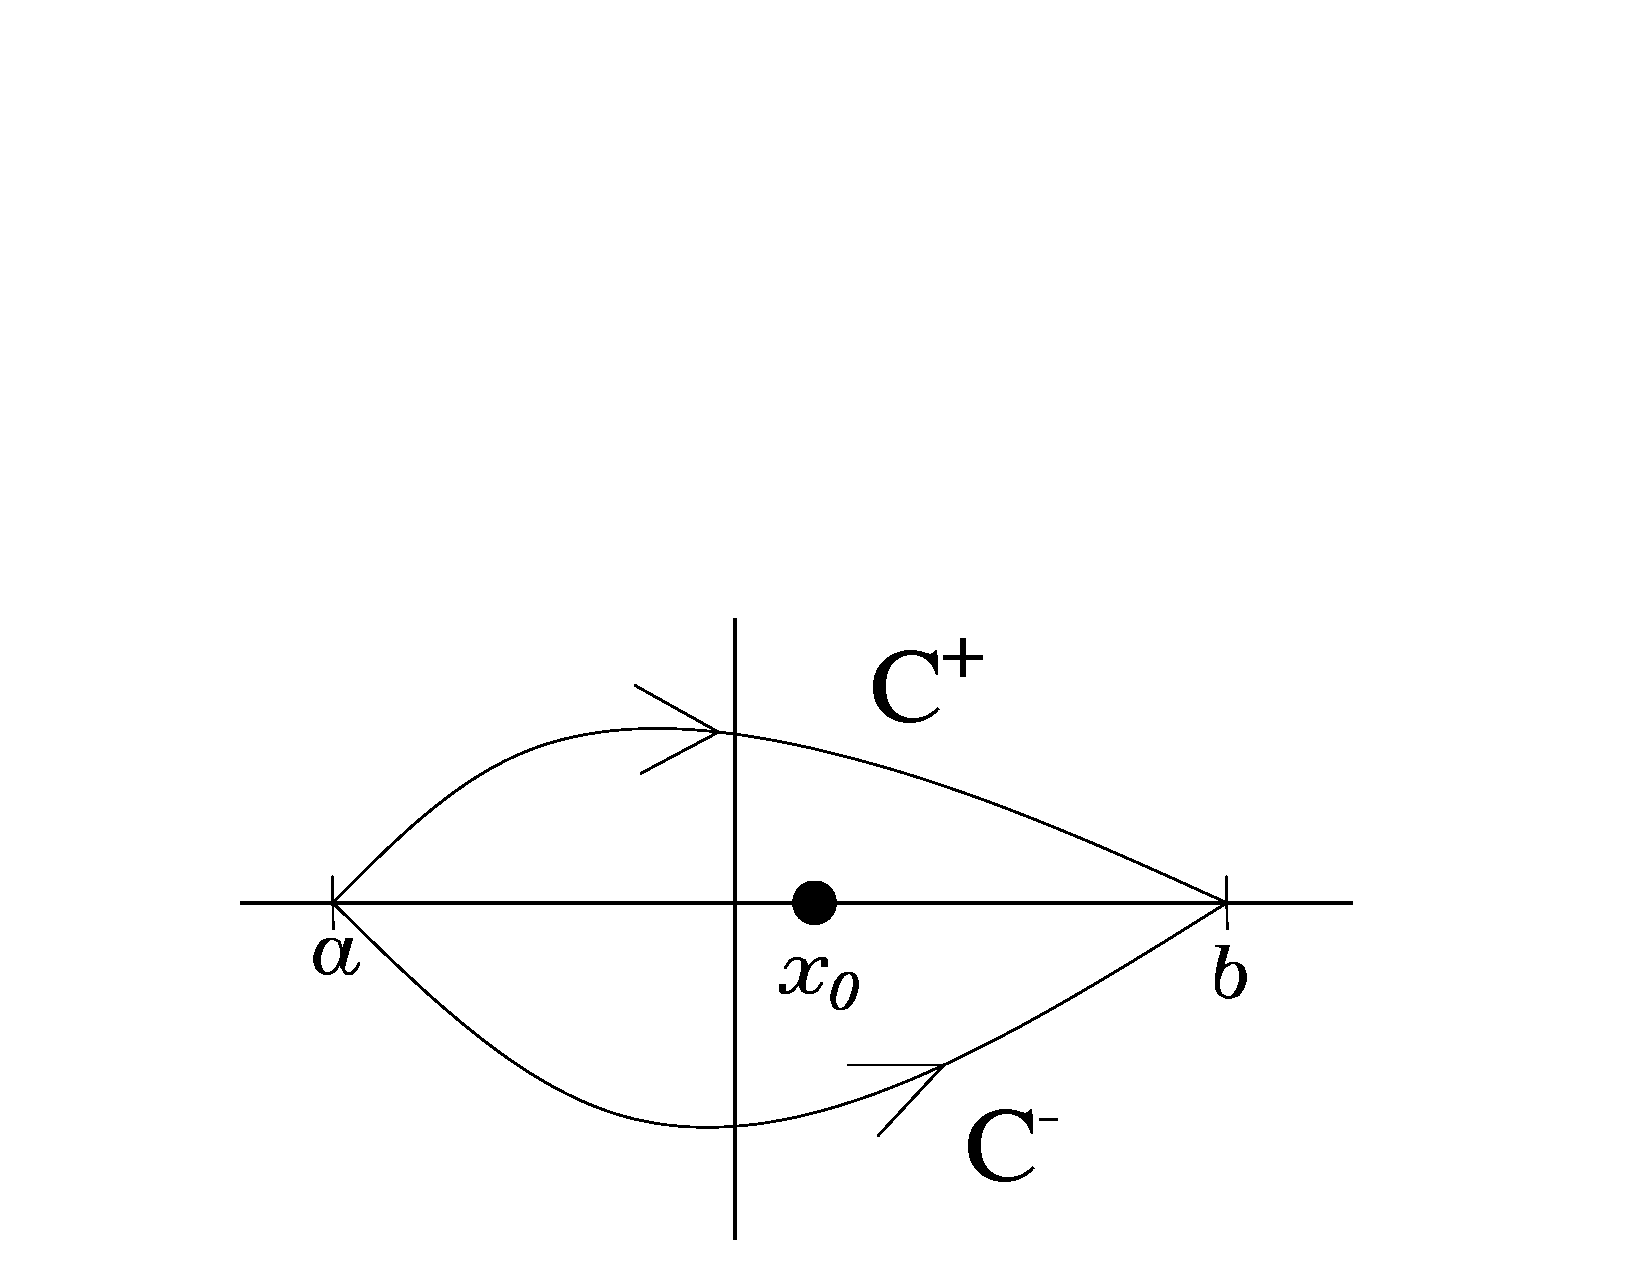
\includegraphics[width=.75\textwidth]{qwer.pdf}
    \caption{The contour $C^{+}$ is an arbitrary contour that runs from $a$ to $b$ above the singularity located at $z=x_0$. While contour $C^{-}$ is an arbitrary contour start from $a$ to $b$ below the singularity at $z=x_0$.}
    \label{APVc}
\end{figure}

\noindent The contour $C^{+}$ runs from $z=a$ to $z=b$ above the singularity $z=x_0$, while $C^{-}$ runs with the same path but below the singularity $z=x_0$, which is shown in Figure \ref{APVc}. It was shown in the same paper that the APV is an equivalent but distinct representation of the Cauchy principal value for $n=0$ and the Hadamard finite-part integral for positive integers $n$. This result gives rise to the heart of the finite-part integration, the complex contour integral representation of the finite part of the divergent integral.

\section{Evaluation of Finite-part Integral}

Consider a standard Stieltjes transform 
 \begin{equation}
     S[f] = \int_0^{\infty} \frac{f(x)}{\omega + x}\, \mathrm{d}x.
\end{equation}
Expanding the kernel $\omega + x$ for small $\omega$ at the origin 
\begin{equation}
    \frac{1}{\omega+x} = \sum_{k=0}^{\infty} (-1)^{k} \frac{\omega^{k}}{x^{k+1}},
\end{equation}
and evaluating the integral by means of term by term integration will result to a family of divergent integrals
 \begin{equation}
     \int_{0}^{\infty} \frac{f(x)}{x^{m+\nu}} \, \mathrm{d}x, \quad m \in \mathbb{N}, \quad 0 \leq \nu < 1, \quad 0 < a \leq \infty
     \label{4.33}
 \end{equation}
for non-integrable singularity at the origin. The divergence of this integral can be removed by replacing the lower limit of integration to some positive $\epsilon$ less than to the upper limit of integration $a$. This will give us the temporary finite-part of the divergent integral and will allow us to group the resulting integral into a pair of terms;
\begin{equation}
    \int_{0}^{a} \frac{f(x)}{x^{m+\nu}} \, \mathrm{d}x = C_\epsilon + D_\epsilon,
\end{equation}
where $C_\epsilon$ is the group of terms that have a finite value when we take the limit of $\epsilon \to 0$ and $D_\epsilon$ is the group of terms that will diverge in the same limit. Dropping the diverging part $D_\epsilon$ will result to the finite-part of the divergent integral. Thus, the limit of the converging terms $C_\epsilon$ is the assigned value of finite-part integral (FPI),
\begin{equation}
    \mathrm{FPI} \, \int_{0}^{a} \frac{f(x)}{x^{m+\nu}} \, \mathrm{d}x = \lim_{\epsilon \to 0} C_\epsilon.
\end{equation}
Equivalently, the finite-part integral can be also expressed in the form of
\begin{equation}
    \mathrm{FPI}  \int_{0}^{a} \frac{f(x)}{x^{m+\nu}} \, \mathrm{d}x, = \lim_{\epsilon \to 0} \, \left[ \int_{\epsilon}^{a} \frac{f(x)}{x^{m+\nu}} \, \mathrm{d}x - D_\epsilon \right].
    \label{FPI2}
\end{equation}
By definition, the limits of the two expression of finite-part integral always exists, and will have a value equal to zero under a certain circumstances. Now, when we extend the upper limit of integration to infinity, $a=\infty$, the finite-part is given by the limit
\begin{equation}
    \mathrm{FPI}  \int_{0}^{\infty} \frac{f(x)}{x^{m+\nu}} \, \mathrm{d}x = \mathrm{FPI} \lim_{a \to \infty} \int_{0}^{a} \frac{f(x)}{x^{m+\nu}} \, \mathrm{d}x.
\end{equation}
To guarantee the existence of the limit of the above equation, it is assumed that the $f(x)x^{-(m+\nu)}$ is integrable at infinity. The order of the evaluation of the limit should be followed strictly. 

To distinguish the familiar notation $\mathrm{FPI} \int_0^{a}$ to the the finite-part of the divergent integral in equation \eqref{4.33}, we will denote it as $\bbint{0}{a}$. This new notation indicate that  we are only dealing to the finite-part integral of the function $f(x)$ with holomorphic complex extensions.

Lastly, one may question the uniqueness of the definition of finite-part integral. To address the ambiguity in the definition, we will discuss it through examples. For example, the term $e^{1/\epsilon}$ appeared after an integration. This term will diverge as we take the limit of $\epsilon \to 0$. If we take $e^{1/\epsilon}$ as a whole, then we need to drop it, and the resulting finite-part is zero. However, if we choose to expand it as  $e^{1/\epsilon} = 1 + 1/\epsilon + 1/2! \epsilon^2 + \ldots$ before performing the limit, we will obtain a non-zero finite-part value. The finite-part value is equal to $1$ because negative exponents of $\epsilon$ will be disregarded since those terms will diverge as we take the limit of $\epsilon \to 0$. Let us consider another example, where we have $\ln (2 \epsilon)$ after performing some integration. Again, if we have taken $\ln (2 \epsilon)$  as a whole, it will give us a zero finite-part value since $\lim_{\epsilon \to 0} \ln(2 \epsilon) = -\infty$. Also, if we take $\ln (2\epsilon) = \ln(2) + \ln(\epsilon)$, it can give us a non-zero finite-part value equal to $\ln(2)$. The term $\ln(\epsilon)$ will be drop since it will diverge as we take the limit of $\epsilon \to 0$. Now, we ask the question, which of the two in each example is the finite-part? This ambiguity of finite-part can be resolve by requiring that the divergent part $D_{\epsilon}$ only take the form of at most the sum of inverse powers of $\epsilon$ and powers of the logarithm $\ln{\epsilon}$. This requirement will result in the finite-part value $1$ and $\ln (2)$ as the desired finite-part for the two examples, respectively. In consequence, the function $f(x)$ is required to have an expansion about $x=0$ in the calculation of finite-part. Similarly, $f(x)$ should be infinitely differentiable at the origin so that it will have a representation in some neighborhood of the origin written as $f(x) = \sum_{k=0}^{\infty} a_k x^{k}$.


\begin{figure}
    \centering
    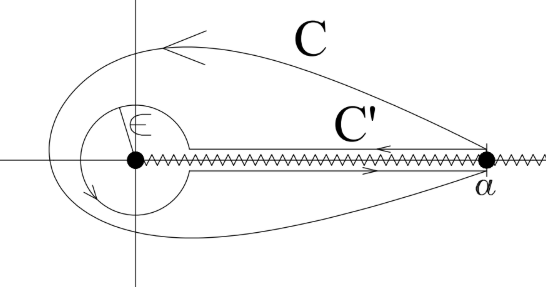
\includegraphics[width=.75\textwidth]{c30.PNG}
    \caption{The contour of integration. The contour $C$ does not enclose any poles or branch points of $f(z)$.}
    \label{ch31}
\end{figure}

\section{Complex Contour Integral Representation of the Finite-part Integral}

Now, it's time to present the heart of the finite-part integration, the contour integral representation of the finite-part integral in the complex plane \cite{galapon2017problem, galapon2016cauchy}. Lifting the finite-part integral to the complex plane requires $f(x)$ to have an analytic complex extension $f(z)$. This contour integral representation is in the form of $\int_{C} f(z) G(z) z^{-m-\nu}$, where $G(z)$ is the function that will induce a branch cut, when necessary. This branch cut runs along the path of integration. The contour $C$ will runs from $a$ and goes back to $a$ to enclose the segment [$0, a$] as shown in Figure \ref{ch31}. The figure is obtained from \cite{doi:10.1063/5.0038274}. The contour $C$ will be deformed in such a way it will straddle the branch cut. The process will lead to a complex contour integral representation of the finite-part integral. Take note that the contour $C$ should not enclosed any pole from $f(z)$ or intersect any branch cuts of $f(z)$.

From the above process, we see that the function $G(z)$ will solely depend on the value of $\nu$. When the value of $\nu$ is zero, the finite-part integral will have a pole in its complex extension. Thus, we need to induce a branch cut that runs along the positive real axis, and we choose that branch cut is from the complex logarithm $\log z$. For the case of $\nu \neq 0$, we do not need to induce a branch cut since the complex extension of the finite-part integral will have a branch point, and we need to choose that the branch cut runs along the positive real axis. Therefore, it is important to know the nature of the divergence of the integrand in the application of finite-part integration. 

The contour integral representation of the two cases and its proof is obtained from \cite{galapon2017problem}.

\subsection{Pole Singularity}

\begin{proposition}
Let $f(x)$ be (m+1) continuously differentiable in the interval $[0,a]$ and $M=sup\{ |f^{(m)}(x)|, x \in [0,a]\} < \infty$. If $f(0) \neq 0$ then we have the finite part integral
\begin{align}
\begin{split}
 \bbint{0}{a} \frac{f(x)}{x^{m+1}} \, \mathrm{d}x & = \lim_{\epsilon \to 0} \Bigg[ \int_\epsilon^a \frac{f(x)}{x^m} \, \mathrm{d}x \\& - \sum_{k=0}^{m-2} \frac{f^{(k)}(0)}{k! (m-1-k)}\frac{1}{\epsilon^{m-1-k}} + \frac{f^{(m-1)}(0)}{(m-1)!} \ln \epsilon \Bigg]
    \label{3.7}
\end{split}
\end{align}
for all $m \in \mathbb{N}$.
\end{proposition}

\begin{proof}
Consider the convergent integral 
\begin{equation}
    \int_\epsilon^a \frac{f(x)}{x^{m+1}} \, \mathrm{d}x
    \label{3.8}
\end{equation}
for $\epsilon \in (0,a)$. Assuming that the function $f(x)$ is differentiable up to $(m+1)$th order. From that assumption, we can write the function $f(x)$ in the form of 
\begin{equation}
    f(x) = \sum_{k=0}^{m} \frac{f^{(k)}(0)}{k!} x^{k} + R_{m+1}(x).
\end{equation}
Substituting the expansion to equation \eqref{3.8} will result to
\begin{equation}
    \int_\epsilon^a \frac{f(x)}{x^{m+1}} \, \mathrm{d}x = \int_\epsilon^{a} \frac{\mathrm{d}x}{x^m+1} \left( \sum_{k=0}^{m-1} \frac{f^{(k)}(0)}{k!}x^{k} + \frac{f^{(m)}(0)}{m!}x^{m} + R_{m+1}(x) \right).
\end{equation}
Then, performing term by term integration will give us
\begin{align}
\begin{split}
    \int_\epsilon^a \frac{f(x)}{x^{m+1}} \, \mathrm{d}x & =- \sum_{k=0}^{m-1} \frac{f^{(k)}(0)}{k!(m-k)} \left( \frac{1}{a^{m-k}} - \frac{1}{\epsilon^{m-k}} \right) \\& +  \frac{f^{(m)}(0)}{m!} \left( \ln a - \ln \epsilon \right) + \int_\epsilon^{a}\frac{R_{m+1}(x)}{x^{m+1}} \mathrm{d}x.
    \label{3.11}
\end{split}
\end{align}
Since the $|R_{m+1}(x)| \leq M|x|^{m+1}/(m+1)! $ for some positive constant M, the integral of the remainder is bounded by 
\begin{equation}
   \left| \int_\epsilon^{a}\frac{R_{m+1}(x)}{x^{m+1}} \mathrm{d}x \right| \leq \int_\epsilon^{a}\frac{|R_{m+1}(x)|}{x^{m+1}} \mathrm{d}x \leq \frac{M}{(m+1)!} (a- \epsilon) \leq \frac{Ma}{(m+1)!}.
\end{equation}
Therefore, the integral of the remainder term exists as we take the limit of $\epsilon \to 0$. Next, we rearrange the equation \eqref{3.11} in such a way we will put the group of the diverging terms to the left and the group of the converging terms to the right as we take the limit of $\epsilon \to 0$.
\begin{align}
\begin{split}
    \int_\epsilon^a & \frac{f(x)}{x^{m+1}} \, \mathrm{d}x  - \sum_{k=0}^{m-1} \frac{f^{(k)}(0)}{k!(m-k)} \frac{1}{\epsilon^{m-k}} + \frac{f^{(m)}(0)}{m!} \ln \epsilon \\& = -\sum_{k=0}^{m-1} \frac{f^{(k)}(0)}{k!(m-k)} \frac{1}{a^{m-k}} +  \frac{f^{(m)}(0)}{m!} \ln a + \int_\epsilon^{a}\frac{R_{m+1}(x)}{x^{m+1}} \mathrm{d}x.
\end{split}
\end{align}
Finally, we reproduce the finite-part integral in equation \eqref{3.7} by taking the limit of $\epsilon \to 0$. Dropping the diverging terms in the LHS will result to Hadamard finite-part integral.
\end{proof}


\begin{theorem} \label{T3.1}
Let the complex extension, $f(z)$, of $f(x)$ be analytic in some neighbourhood of the interval $[0, a]$. If $f(0) \neq 0$ and $m = 0,1,2,...$, then
\begin{equation}
    \bbint{0}{a} \frac{f(x)}{x^{m+1}} \, \mathrm{d}x = \frac{1}{2 \pi i} \int_{C} \frac{f(z)}{z^{m+1}} (\log z - \pi i) \, \mathrm{d}z
\end{equation}
where $\log z$ is the complex logarithm whose branch cut is the positive real axis and $C$ is the contour straddling the branch cut of $\log z$ starting from $a$ and ending at $a$ itself, as depicted in Figure \ref{ch31}.
\end{theorem}

\begin{proof}
First, we will consider the complex contour integral 
\begin{equation}
    \int_{C} \frac{f(z)}{z^{m+1}} \log z \, \mathrm{d}z
\end{equation}
where the contour $C$ is shown in the Figure \ref{ch32} and will be deformed into $C'$. The complex contour integral will be evaluated along the deformed $C'$ and will give us
\begin{equation}
    \int_{C} \frac{f(z)}{z^{m+1}} \log z \, \mathrm{d}z = \int_a^{\epsilon} \frac{f(x) \log x}{x^{m+1}} \, \mathrm{d}x + \int_{\epsilon} \frac{f(z) \log z}{z^{m+1}} \, \mathrm{d}z + \int_\epsilon^a \frac{f(x) \log (x \mathrm{e}^{2 \pi i})}{x^{m+1}} \, \mathrm{d}x.       
\end{equation}
The first term represent the path above the branch cut  induced by $\log z$, the second is the small circle about the origin, and the third term is the path below the branch cut. Using the logarithmic property, it will give as the relation $\log \,x = \log \, x + 2 \pi i$ and will simplify the equation into 
\begin{equation}
    \int_{C} \frac{f(z)}{z^{m+1}} \log z \, \mathrm{d}z = 2 \pi i \int_{\epsilon}^a \frac{f(x)}{x^{m+1}} \, \mathrm{d}x + \int_{\epsilon} \frac{f(z) \log z}{z^{m+1}} \, \mathrm{d}z  . 
    \label{3.18}
\end{equation}

Now, we will evaluate the integral along the small circle by expanding first the function $f(z)$ at $z=0$, which give us
\begin{equation}
    f(z) = \sum_{k=0}^{m} \frac{f^{(k)}(0)}{k!} z^k + \mathcal{O}(z^{m+1}), m = 0,1,....
\end{equation}
since by assumption it is analytic at $z=0$. Substituting it back to the integral and using the parameterization $z = \epsilon \mathrm{e}^{i \theta}$, $0 \leq \theta < 2 \pi$ and via logarithmic property, we use the relation $\log(x \mathrm{e}^{i \theta}) = \log x + i \theta$  and obtain
\begin{align}
\begin{split}
    \int_{\epsilon} \frac{f(z) \log z}{z^{m+1}} \,  \mathrm{d}z & = \sum_{k=0}^m \frac{f^{(k)}(0)}{k!} \frac{1}{\epsilon^{m-k}} \bigg[ i \ln \epsilon \int_0^{2 \pi} \mathrm{e}^{-i(m-k)\theta} \mathrm{d}\theta \\& - \int_0^{2 \pi} \mathrm{e}^{-i(m-k)\theta} \theta \mathrm{d}\theta  \bigg] + \mathcal{O}(\epsilon).
    \label{3.20}
\end{split}
\end{align}
the above integral will be evaluated using these known integrals:
\begin{equation}
    \int_0^{2 \pi} \mathrm{e}^{-i(m-k)\theta} \, \mathrm{d}\theta = 
    \begin{cases} 
      0, & m \neq k \\
      2 \pi, & m = k
   \end{cases}
\end{equation}
and
\begin{equation}
    \int_0^{2 \pi} \mathrm{e}^{-i(m-k)\theta} \theta \, \mathrm{d}\theta =     \begin{cases} 
      \frac{2 \pi i}{m-k}, & m \neq k \\
      2 \pi^2, & m = k
   \end{cases} .
\end{equation}
Substituting the integrals above to equation \eqref{3.20}, will result to
\begin{align}
\begin{split}
    \int_{\epsilon} \frac{f(z) \log z}{z^{m+1}} \,  \mathrm{d}z & = 2 \pi i \left[ \frac{f^{(m)}(0)}{m!} \ln \epsilon - \sum_{k=0}^{m-1} \frac{f^{(k)}(0)}{k!(m-k) \epsilon^{m-k}} \right] \\& - 2 \pi^{2} \frac{f^{(m)}(0)}{(m-1)!} + \mathcal{O}(\epsilon).
    \label{3.23}
\end{split}
\end{align}
Since we already evaluated the integral along the small circle about the origin, we will substitute it back to the contour integral in equation \eqref{3.18} that will result to
\begin{align}
\begin{split}
     \int_{C} & \frac{f(z)}{z^{m+1}} \log z \, \mathrm{d}z = 2 \pi i \bigg[ \int_{\epsilon}^a \frac{f(x)}{x^{m+1}} \, \mathrm{d}x +  \frac{f^{(m)}(0)}{m!} \ln \epsilon \\&  - \sum_{k=0}^{m-1} \frac{f^{(k)}(0)}{k!(m-k) \epsilon^{m-k}} \bigg] - 2 \pi^{2} \frac{f^{(m)}(0)}{(m)!} + \mathcal{O}(\epsilon).
    \label{3.24}
\end{split}
\end{align}
We will manipulate the last term in the right-hand side of the equation as
\begin{equation}
    2 \pi^{2} \frac{f^{(m)}(0)}{(m)!} = \frac{\pi}{i} \int_{C} \frac{f(z)}{z^{m+1}} \, \mathrm{d}z = -\pi i \int_C \frac{f(z)}{z^m} \, \mathrm{d}z.
\end{equation}
Substituting the manipulated last term to the equation \eqref{3.24} and dividing both sides by $2 \pi i$ will result to 
\begin{align}
\begin{split}
     \frac{1}{2 \pi i}\int_{C} & \frac{f(z)}{z^{m+1}} (\log z - \pi i) \, \mathrm{d}z = \int_{\epsilon}^a \frac{f(x)}{x^{m+1}} \, \mathrm{d}x +  \frac{f^{(m)}(0)}{m!} \ln \epsilon \\&  - \sum_{k=0}^{m-1} \frac{f^{(k)}(0)}{k!(m-k) \epsilon^{m-k}} + \mathcal{O}(\epsilon).
\end{split}
\end{align}
Taking the limit of $\epsilon \to 0^{+}$, we recognize that the right-hand side is the definition of the Hadamard finite part in equation \eqref{3.7}. Therefore, 
\begin{equation}
    \bbint{0}{a} \frac{f(x)}{x^{m+1}} \, \mathrm{d}x = \frac{1}{2 \pi i} \int_C \frac{f(z)}{z^{m+1}} (\log z - \pi i) \, \mathrm{d}z,
\end{equation}
for  $m = 0, 1,2, ...$.
\end{proof}

\subsection{Branch Point Singularity}
\begin{proposition}
Let $f(x)$ be n continuously differentiable in the interval $[0,a]$ and $M=sup\{ |f^{(n)}(x)|, x \in [0,a]\} < \infty$. If $f(0) \neq 0$ then we have the finite part integral
\begin{align}
\begin{split}
    \bbint{0}{a} \frac{f(x)}{x^{n+\nu}} \, \mathrm{d}x & = \lim_{\epsilon \to 0^{+}} \Bigg[ \int_\epsilon^a \frac{f(x)}{x^m} \, \mathrm{d}x \\& - \sum_{l=0}^{m-1} \frac{f^{(l)}(0)}{l! (n+\nu-l-1)}\frac{1}{\epsilon^{n+\nu-l-1}} \Bigg] 
\label{P2}
\end{split}
\end{align}
for all $n \in \mathbb{N}$ and $\nu \in (0,1)$.
\end{proposition}

\begin{proof}
Similar to the case of pole singularity, we will consider an integral in the form of 
\begin{equation}
    \int_\epsilon^a \frac{f(x)}{x^{n+ \nu}} \, \mathrm{d}x
    \label{3.29}
\end{equation}
for $\epsilon \in (0,a)$. Since we let $f(x)$ to be $n$th differentiable along the integral, we can expand it at the origin via the Taylor series expansion given by
\begin{equation}
    f(x) = \sum_{k=0}^{n-1} \frac{f^{(k)}(0)}{k!} \, x^{k} + R_{n}(x)
\end{equation}
Substituting this expansion to the integral we considered in \eqref{3.29}, and integrating it, will result to
\begin{align}
\begin{split}
    \int_\epsilon^a \frac{f(x)}{x^{n+ \nu}} \, \mathrm{d}x & = \sum_{k=0}^{n-1} \frac{f^{(k)}(0)}{k!(k-n-\nu+1)} \, \left( \frac{1}{a^{n+\nu-k-1}} - \frac{1}{\epsilon^{n+\nu-k-1}} \right) \\& + \int_\epsilon^a \frac{R_{n}(x)}{x^{n+\nu}} \, \mathrm{d}x. 
    \label{3.31}
\end{split}
\end{align}
Next, we need to find out if the remainder term has a finite limit as we take $\epsilon \to 0$. Using the bound for the remainder term $R_n{x} \leq M |x|^{n}/n!$ for some positive constant $M$.  The bound for the integral involving the remainder is given by
\begin{equation}
    \left| \int_\epsilon^a \frac{R_{n}(x)}{x^{n+\nu}} \, \mathrm{d}x \right| \leq \int_\epsilon^a \frac{|R_{n}(x)|}{x^{n+\nu}} \, \mathrm{d}x \leq \frac{M}{n!(1-\nu)} (a^{1-\nu} - \epsilon^{1-\nu})
\end{equation}
since $\nu \in (0,1)$, the integral consisting of the the remainder term exists as $\epsilon \to 0$. Now, we will rearrange the terms on equation \eqref{3.31} in such away, the group of the diverging in term is in the left-hand side and the group of converging term is in the right-hand side as we take the limit of $\epsilon \to 0$. The resulting equation is 
\begin{align}
\begin{split}
    \int_\epsilon^a & \frac{f(x)}{x^{n+ \nu}} \, \mathrm{d}x + \sum_{k=0}^{n-1} \frac{f^{(k)}(0)}{k!(k-n-\nu+1)} \, \frac{1}{\epsilon^{n+\nu-k-1}} \\&  = \sum_{k=0}^{n-1} \frac{f^{(k)}(0)}{k!(k-n-\nu+1)} \, \frac{1}{a^{n+\nu-k-1}} + \int_\epsilon^a \frac{R_{n}(x)}{x^{n+\nu}} \, \mathrm{d}x. 
\end{split}
\end{align}
 Therefore, we reproduced the equation in equation $\eqref{P2}$.
\end{proof}

\begin{theorem}\label{T3.2}
Let the complex extension, $f(z)$, of $f(x)$ be analytic in some neighbourhood of the interval $[0, a]$. If $f(0) \neq 0$ for all $n \in \mathbb{N}$ and $0 < \nu < 1$, then 
\begin{equation}
    \bbint{0}{a} \frac{f(x)}{x^{n+\nu}} \, \mathrm{d}x = \frac{1}{\mathrm{e}^{-2 \pi \nu i}-1} \int_C \frac{f(z)}{z^{n+\nu}} \, \mathrm{d}z
\end{equation}
where the branch of $z^{-\nu}$ is such that it is positive on top of the positive real axis and the contour $C$ is the contour straddling the branch cut of $z^{-\nu}$ starting from $a$ and ending at $a$ itself, as depicted in Figure \ref{ch31}.
\end{theorem}
\begin{proof}
In order to prove the theorem, we will consider the complex integral
\begin{equation}
    \int_C \frac{f(z)}{z^{n+\nu}} \, \mathrm{d}z
\end{equation}
where the contour is shown in Figure \ref{ch32}. The contour will be deformed as $C'$ and evaluating it
\begin{align}
\begin{split}
    \int_C \frac{f(z)}{z^{n+\nu}} \, \mathbb{d}z & = \int_{a}^{\epsilon} \frac{f(x)}{x^{n+\nu}} \, \mathrm{d}x + \int_{\epsilon} \frac{f(z)}{z^{n+\nu}} \, \mathrm{d}z + \int_{a}^{\epsilon} \frac{f(x)}{x^{n+\nu} \mathrm{e}^{2 \pi \nu}} \, \mathrm{d}x \\& = (\mathrm{e}^{-2 \pi \nu i}-1) \int_{a}^{\epsilon} \frac{f(x)}{x^{n+\nu}} \, \mathrm{d}x + \int_{\epsilon} \frac{f(z)}{z^{n+\nu}} \, \mathrm{d}z.
    \label{3.36}
\end{split}
\end{align}
For the evaluation of the integral along the circle about the origin, we will have a parameterization of $z = \epsilon \mathrm{e}^{i \epsilon}$, $0 \leq \theta \leq 2 \pi$. Moreover, since we assume that $f(z)$ is analytic along the contour. We can expand $f(z)$ it as a Taylor series at the origin, given by
\begin{equation}
    f(z) = \sum_{k=0}^{n-1} \frac{f^{(k)}(0)}{k!}(\epsilon \mathrm{e}^{i \theta})^{k} + \mathcal{O}((\epsilon \mathrm{e}^{i \theta})^{n}).
\end{equation}
From that, the integral along the circle about the origin is evaluated to be
\begin{align}
\begin{split}
	\int_{\epsilon} & \frac{f(z)}{z^{n+\nu}}\mathrm{d}z = \int_{0}^{2\pi}\frac{1}{\left(\epsilon e^{i\theta}\right)^{n+\nu}}\left(\sum_{k=0}^{n-1}\frac{f^{k}(0)}{k!}\left(\epsilon e^{i\theta}\right)^{k}+\mathcal{O}\left(\left(\epsilon e^{i\theta}\right)^{n}\right)\right)\epsilon i e^{i\theta}\mathrm{d}\theta
	\\& =  \sum_{k=0}^{n-1}\frac{f^{(k)}(0)}{k!\,\epsilon^{n+\nu-k-1}}\,i\int_{0}^{2\pi} e^{-i\theta(n+\nu-k-1)}\mathrm{d}\theta + i\,\epsilon^{1-\nu} \int_{0}^{2\pi}\mathcal{O}\left(\left( e^{i\theta}\right)^{1-\nu}\right)\mathrm{d}\theta.
\end{split}
\end{align}
Performing the integration
\begin{equation}
	\int_{\epsilon}\frac{f(z)}{z^{n+\nu}}\mathrm{d}z = -\sum_{k=0}^{n-1}\frac{f^{(k)}(0)}{k!\,\left(n+\nu-k-1\right)\,\epsilon^{n+\nu-k-1}}\left(e^{-2\pi\nu i}-1\right) + \mathcal{O}(\epsilon^{1-\nu}).
	\label{3.39}
\end{equation}
Since we already simplify the integral along the circle, we will substitute it back to equation $\eqref{3.36}$. Taking the limit as $\epsilon \to 0^{+}$ will make the order term vanishes since $\nu < 1$. Then, dividing both sides by $\mathrm{e}^{-2 \pi \nu i} -1$ will result to
	\begin{equation}
		\frac{1}{\left(e^{-2\pi\nu i}-1\right)}\int_{C}\frac{f(z)}{z^{n+\nu}}\mathrm{d}z =\lim_{\epsilon\to 0}\left( \int_{\epsilon}^{a}\frac{f(x)}{x^{n+\nu}}\mathrm{d}x -\sum_{k=0}^{n-1}\frac{f^{(k)}(0)}{k!\,\left(n+\nu-k-1\right)\,\epsilon^{n+\nu-k-1}}\right).
	\end{equation}
The RHS of the above equation is recognized to be the Hadamard finite-part integration according to \eqref{P2}. Thus, we obtain the contour integral representation of the finite-part integral for the branch point singularity. 
\end{proof}


\section{Finite-part  Integration  of  the  Generalized  Stieltjes  Transform  of an Entire  Function}

In this section, we will show how we implement the method to exactly evaluate the generalized Stieltjes transform of an entire function with an integral \cite{tica2018finite} and non-integral orders \cite{tica2019finite}.

\subsection{Finite-Part Integration of the Generalized Stieltjes Transform of an Entire Function with Integral Order}


%Figure
\begin{figure}
    \centering
    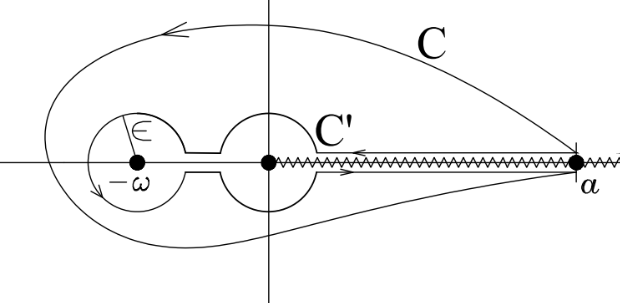
\includegraphics[width=.75\textwidth]{c31.PNG}
    \caption{The contour of integration with pole at $-\omega$, branch point at the origin, and branch cut runs from $(0,\infty)$. The contour encloses the pole at $-\omega$.}
    \label{ch32}
\end{figure}

Consider an incomplete generalized Stieltjes transform of integral order 
\begin{equation}\label{lb}
	S_{n}^{a}[f(x)] = \int_{0}^{a}\frac{f(x)}{(\omega+x)^{n}}\mathrm{d}x,
\end{equation} 
where $f(x)$ has an entire complex extension. We will have a pole at $z = -\omega$, when the integral is lifted to the complex plane. Recall from the previous discussion, we need to induce a branch cut along the positive real axis. From that, we will consider a contour integral 
\begin{equation}
    \int_C \frac{f(z)}{(\omega +z)^{n}} \log z \, \mathrm{d}z
\end{equation}
where the contour $C$ if in the Figure \ref{ch32}. Deforming the contour $C$ to $C'$ and evaluating it, will give us the equation
\begin{align}
\begin{split}
    \int_C & \frac{f(z)}{(\omega +z)^{n}} \log z \, \mathrm{d}z = \int_{a}^{\epsilon} \frac{f(x)}{(\omega +x)^{n}} \log x \mathrm{d}x + \int_\epsilon  \frac{f(z)}{(\omega +z)^{n}} \log z \, \mathrm{d}z \\& + \int_{\epsilon}^{a} \frac{f(x)}{(\omega +x)^{n}} (\log x + 2 \pi i) \mathrm{d}x + 2 \pi i \, \mathrm{Res} \left[\frac{f(z)}{(\omega +z)^{n}} \log z \,  \right]_{z=-\omega}.
\end{split}
\end{align}
Letting $\epsilon \to 0$ will make the term with the integral along the circle vanish that can be shown using L'hopitals rule. Now, combining similar terms will further simplify the equation
\begin{align}
\begin{split}
    \int_C & \frac{f(z)}{(\omega +z)^{n}} \log z \, \mathrm{d}z = 2 \pi i \int_{\epsilon}^{a} \frac{f(x)}{(\omega +x)^{n}} \mathrm{d}x  \\& + 2 \pi i\mathrm{Res} \left[\frac{f(z)}{(\omega +z)^{n}} \log z \,  \right]_{z=-\omega}.
\end{split}
\end{align}
Rearranging the equation in such a way we obtain the generalized Stieltjes transform in equation \eqref{lb} and dividing both sides by $2 \pi i$ will result to
\begin{align}
\begin{split} \label{3.47}
    \int_{\epsilon}^{a} & \frac{f(x)}{(\omega +x)^{n}} \mathrm{d}x = \frac{1}{2 \pi i} \int_C \frac{f(z)}{(\omega +z)^{n}} \log z \, \mathrm{d}z  \\& - \mathrm{Res} \left[\frac{f(z)}{(\omega +z)^{n}} \log z \,  \right]_{z=-\omega}.
\end{split}
\end{align}
The residue can be rewritten to its differential form express by the equation
\begin{equation}
	\mathrm{Res}\left[\frac{f\left(z\right)\log z}{\left(\omega+z\right)^n}\right]_{z=-\omega}= \left. \frac{1}{\left(n-1\right)!}\frac{\mathrm{d}^{n-1}}{\mathrm{d}z^{n-1}}\left(f\left(z\right)\log z\right)\right|_{z=-\omega}.
\end{equation}
This differential form can be calculated using the Leibniz rule or the generalized product rule. Applying it will result to
\begin{align}
\begin{split}
		\mathrm{Res}&\left[\frac{f\left(z\right)\log z}{\left(\omega+z\right)^n}\right]_{z=-\omega}  = \frac{1}{\left(n-1\right)!}\sum_{k=0}^{n-1}{n-1\choose k}f^{\left(k\right)}\left(-\omega\right)\left. \frac{\mathrm{d}^{n-1-k}}{\mathrm{d}z^{n-1-k}}\log z\right|_{z=-\omega}.
\end{split}
\end{align}
Now, we will separate the $k=n-1$ term from the summation and perform the differentiation,
\begin{align}
\begin{split}
		\mathrm{Res}&\left[\frac{f\left(z\right)\log z}{\left(\omega+z\right)^n}\right]_{z=-\omega}  = \\& \quad \frac{1}{\left(n-1\right)!}\sum_{k=0}^{n-2}{n-1\choose k}f^{\left(k\right)}\left(-\omega\right)\left[\frac{\mathrm{d}^{n-2-k}}{\mathrm{d}z^{n-2-k}}\,z^{-1} \right]_{z=-\omega} \\&
		 +\, \frac{f^{\left(n-1\right)}\left(-\omega\right)}{\left(n-1\right)!}\ln \omega\, +\, \pi i\,\frac{f^{\left(n-1\right)}\left(-\omega\right)}{\left(n-1\right)!}.
\end{split}
\end{align}
Using this following relation
\begin{equation}
	\frac{\mathrm{d}^{n}\,z^{-1}}{\mathrm{d}z^{n}}=\left(-1\right)^{n}\left(n!\right)z^{-n-1}\qquad\text{and}\qquad{n-1\choose k}=\frac{\left(n-1\right)!}{k!\,\left(n-1-k\right)!},
\end{equation}
and the Cauchy integral formula,
\begin{equation}
	f^{\left(n-1\right)}\left(-\omega\right)=\frac{\left(n-1\right)!}{2\pi i}\int_{C}\frac{f\left(z\right)}{\left(\omega+z\right)^n}\mathrm{d}z
\end{equation}
we successfully evaluate the residue at $z = -\omega$
\begin{align}
\begin{split}\label{esd}
	\mathrm{Res}&\left[\frac{f\left(z\right)\log z}{\left(\omega+z\right)^n}\right]_{z=-\omega}  = -\sum_{k=0}^{n-2}\frac{f^{\left(k\right)}\left(-\omega\right)\left(n-2-k\right)!\left(\omega\right)^{k-n+1}}{k!\,\left(n-1-k\right)!} \\& \hspace{25mm}
	 +\,\,\frac{f^{\left(n-1\right)}\left(-\omega\right)}{\left(n-1\right)!}\ln\omega\;+\;\frac{\pi i}{2\pi i}\int_{C}\frac{f\left(z\right)}{\left(\omega+z\right)^n}\mathrm{d}z.
\end{split}
\end{align}
Substituting the evaluated residue \eqref{esd} into equation \eqref{3.47} will result to
\begin{align}
\begin{split} \label{piyo}
	\int_{0}^{a} & \frac{f\left(x\right)}{\left(\omega+x\right)^n}\mathrm{d}x
	=\frac{1}{2\pi i}\int_{C}\frac{f\left(z\right)\left(\log z-\pi i\right)}{\left(\omega+z\right)^n}\mathrm{d}z \\& -\frac{f^{\left(n-1\right)}\left(-\omega\right)}{\left(n-1\right)!}\ln\omega
	+\omega^{1-n}\sum_{k=0}^{n-2}\frac{f^{\left(k\right)}\left(-\omega\right)\left(\omega\right)^{k}}{k!\,\left(n-1-k\right)}.
\end{split}
\end{align}
 Thus, we show that the contribution of the residue is just 
 \begin{eqnarray} \label{Res}
 \Delta_{\mathrm{sc}}^{(n)}(\omega)&=&-\;\frac{1}{\left(n-1\right)!}f^{(n-1)}\!\left(-\omega\right)\, \ln\omega \nonumber \\
 && + \sum_{k=0}^{n-2}\frac{f^{\left(k\right)}\left(-\omega\right)}{k!\,\left(n-1-k\right) \; \omega^{n-k-1}}, \;\;\; n=2, 3, \dots.
 \end{eqnarray}
For the contour integral in the first term in the right-hand side. We will expand the binomial $\omega + z$ using the binomial expansion
\begin{equation}
	\frac{1}{\left(\omega+z\right)^{n}}=\frac{1}{z^n}\sum_{k=0}^{\infty}{{-n}\choose k}\left(\frac{\omega}{z}\right)^{k}.
\end{equation}
Inserting this expansion to equation \eqref{piyo} will result to
\begin{align}
\begin{split}
	\int_{0}^{a} & \frac{f\left(x\right)}{\left(\omega+x\right)^n}\mathrm{d}x = \frac{1}{2\pi i}\int_{C}\frac{f\left(z\right)\left(\log z-\pi i\right)}{\left(z\right)^n}\sum_{k=0}^{\infty}{{-n}\choose k}\left(\frac{\omega}{z}\right)^{k}\mathrm{d}z
	\\& \hspace{25mm}-\frac{f^{\left(n-1\right)}\left(-\omega\right)}{\left(n-1\right)!}\ln\omega
	+\omega^{1-n}\sum_{k=0}^{n-2}\frac{f^{\left(k\right)}\left(-\omega\right)\left(\omega\right)^{k}}{k!\,\left(n-1-k\right)}.
\end{split}
\end{align}
The expansion is uniformly convergent for $|z| > \omega$. Since the contour integral is uniformly convergent in that case, the interchanging of order of the integration and summation is allowed
\begin{align}
\begin{split}
	\frac{1}{2\pi i}\int_{C} & \frac{f\left(z\right)\left(\log z-\pi i\right)}{\left(\omega+z\right)^n} \mathrm{d}z
	 =\\& \sum_{k=0}^{\infty}{-n\choose k}\omega^{k}\frac{1}{2\pi i}\int_{C}\frac{f\left(z\right)\left(\log z-\pi i\right)}{z^{n+k}}\mathrm{d}z.
\end{split}
\end{align}
By the virtue of the Theorem \ref{T3.1}, we express the complex contour integral as a finite-part integral
\begin{equation}
	\sum_{k=0}^{\infty}{-n\choose k}\omega^{k}\frac{1}{2\pi i}\int_{C}\frac{f\left(z\right)\left(\log z-\pi i\right)}{z^{n+k}}\mathrm{d}z = \sum_{k=0}^{\infty}{-n\choose k}\omega^{k}\,\bbint{0}{a}\frac{f\left(x\right)}{x^{n+k}}\mathrm{d}x.
\end{equation} 
Combining all the results will lead us to the theorem found in \cite{tica2018finite}.
\begin{theorem} \label{T3.3}
 	Let the complex extension, $f(z)$, of $f(x)$ be entire. Then for all $n = 1, 2, 3, \dots$ and $0<\omega<a$, the following equality holds
 	\begin{equation}
 	\int_0^a \frac{f(x)}{(\omega + x)^n} \mathrm{d}x = \sum_{k=0}^{\infty} \binom{-n}{k} \omega^{ k} \bbint{0}{a} \frac{f(x)}{x^{k + n}}\mathrm{d}x + \Delta_{\mathrm{sc}}^{(n)}(\omega)
 	\end{equation}
 	where
 	\begin{eqnarray}\label{singular_terrmm}
 	\Delta_{\mathrm{sc}}^{(n)}(\omega)&=&-\;\frac{1}{\left(n-1\right)!}f^{(n-1)}\!\left(-\omega\right)\, \ln\omega \nonumber \\
 	&& + \sum_{k=0}^{n-2}\frac{f^{\left(k\right)}\left(-\omega\right)}{k!\,\left(n-1-k\right) \; \omega^{n-k-1}}, \;\;\; n=2, 3, \dots \label{main1sub}.
 	\end{eqnarray}
 \end{theorem}

In addition, to just explicitly show that the interchanging of order of the summation and integration is valid, we need to establish the absolute convergence of the series. To do this, we will deform the contour $C$ into a circle of radius $a$ about the origin and obtain this following bound,
 \begin{eqnarray}
 \left|\bbint{0}{a} \frac{f(x)}{x^{k+n}}\mathrm{d}x\right| &=& \left|\frac{1}{2\pi i}\int_{\mathrm{C}} \frac{f(z)}{z^{k+n}} (\log z - i\pi) \mathrm{d}z\right|\nonumber \\
 &=& \left|\frac{1}{2\pi i} \int_0^{2\pi} \frac{f(a e^{i\theta})}{a^{k + n} e^{i(k+n)\theta}} (\ln a + (\theta - \pi)i) i a e^{i\theta} \mathrm{d}\theta\right|\nonumber \\
 &\leq & \frac{1}{a^{k+n - 1}} \frac{1}{2\pi} \int_0^{2\pi} \left|f(ae^{i\theta})(\ln a + (\theta - \pi)i)  \mathrm{d}\theta\right| \nonumber \\
 &\leq& \frac{1}{a^{k+n-1}} M(a)
 \end{eqnarray}
 where $M(a) > 0$ is a finite constant independent of $k$. Finally,  We will have a bound
\begin{eqnarray}\label{delta2}
\left|\sum_{k=0}^{\infty} \binom{-n}{k} \omega^{ k} \bbint{0}{a} \frac{f(x)}{x^{k  +1}}\mathrm{d}x\right|&\leq& \sum_{k=0}^{\infty} \left|\binom{-n}{k}\right| \omega^{k} \left|\bbint{0}{a} \frac{f(x)}{x^{k  +1}}\mathrm{d}x\right| \nonumber \\
&\leq& \frac{M(a)}{a^{n-1}}\sum_{k=0}^{\infty} \binom{n+k-1}{k} \frac{\omega^{ k}}{a^{k}} \nonumber \\
&=& \frac{a M(a)}{(a - \omega)^n},
\end{eqnarray}
 for the case $a>\omega$ since the infinite series converges absolutely.

 
\subsection{Finite-Part Integration of the Generalized Stieltjes Transform of an entire function with Branch Point at the Origin}

Next, we will try to implement the method of finite-part integration to the generalized Stieltjes transform of $x^{-\nu} f(x)$  
\begin{equation}\label{bl}
		S_{n}^{a}[x^{-\nu}f(x)] = \int_{0}^{a}\frac{x^{-\nu}\,f(x)}{(\omega+x)^{n}}\mathrm{d}x,
\end{equation}
where $f(x)$ has an entire complex extension $f(z)$. Lifting the integral of interest to the complex plane will induce a branch point at the origin due to the factor $x^{-\nu}$. We choose that the branch cut runs along the positive real axis. Therefore, we will have a contour integral written as
\begin{equation}
    \int_C \frac{z^{-\nu} f(z)}{(\omega + z)^{n}} \, \mathrm{d}z
\end{equation}
where contour $C$ is shown in Figure \ref{ch32}. Similar to the previous subsection, the contour will be deformed into $C'$ and evaluated to be
\begin{align}
\begin{split}
    \int_{C} & \frac{z^{-\nu}\,f\left(z\right)}{\left(\omega+z\right)^{n}}\,\mathrm{d}z =  \int_{a}^{\epsilon}\,\frac{x^{-\nu}\,f\left(x\right)}{\left(\omega+z\right)^{n}}\,\mathrm{d}x + \int_\epsilon \frac{z^{-\nu}\,f\left(z\right)}{\left(\omega+z\right)^{n}}\,\mathrm{d}z + \\& e^{-2\,\pi \nu i} \int_{\epsilon}^a\,\frac{x^{-\nu}\,f\left(x\right)}{\left(\omega+z\right)^{n}}\,\mathrm{d}x + 2 \pi i \, \mathrm{Res}\left[\frac{z^{-\nu}\,f\left(z\right)}{\left(\omega+z\right)^{n}}\,\right]_{z=-\omega}.
\end{split}
\end{align}
Combining similar terms and letting $\epsilon \to 0$ will simplify the equation to
\begin{align}
\begin{split}
    \int_{C} & \frac{z^{-\nu}\,f\left(z\right)}{\left(\omega+z\right)^{n}}\,\mathrm{d}z = (e^{-2\,\pi \nu i} - 1) \int_{\epsilon}^{a}\,\frac{x^{-\nu}\,f\left(x\right)}{\left(\omega+z\right)^{n}}\,\mathrm{d}x \\& + 2 \pi i \, \mathrm{Res}\left[\frac{z^{-\nu}\,f\left(z\right)}{\left(\omega+z\right)^{n}}\,\right]_{z=-\omega} .
\end{split}
\end{align}
Rearranging the terms in such a way we will obtain the desired integral and dividing both sides by $e^{-2\,\pi \nu i} - 1$ will lead to
\begin{align}
\begin{split} \label{3.69}
	\int_{0}^{a}\,&\frac{x^{-\nu}\,f\left(x\right)}{\left(\omega+z\right)^{n}}\,\mathrm{d}x=\frac{1}{e^{-2\pi\,\nu\,i}-1}\int_{C}\frac{z^{-\nu}\,f\left(z\right)}{\left(\omega+z\right)^{n}}\,\mathrm{d}z\\&-\frac{2\pi\,i}{e^{-2\,\pi\,i}-1}\mathrm{Res}\left[\frac{z^{-\nu}\,f\left(z\right)}{\left(\omega+z\right)^{n}}\,\right]_{z=-\omega}.
\end{split}
\end{align}
Simplifying the factor of the second term or the residue using the Euler Identity will give us 
\begin{align}
\begin{split}
	\frac{2\pi\,i}{e^{-2\pi\,\nu\,i}-1} &=\frac{2\pi\,i}{\left(e^{-\pi\,\nu\,i}-e^{\pi\,\nu\,i}\right)\,e^{-\pi\,\nu\,i}} \\& =\frac{2\pi\,i}{-2\,i\sin\left(\pi\,\nu\right)\,e^{-\pi\,\nu\,i}} \\& =\frac{-\pi}{\sin\left(\pi\,\nu\right)\,e^{-\pi\,\nu\,i}}.
\end{split}
\end{align}
We will now evaluate the residue via the Leibniz rule
\begin{eqnarray}\nonumber
	\mathrm{Res}\left[\frac{z^{-\nu}\,f\left(z\right)}{\left(\omega+z\right)^{n}}\,\right]_{z=-\omega} &=&\frac{1}{\left(n-1\right)!}\,\frac{\mathrm{d}^{n-1}}{\mathrm{d}z^{n-1}}\,\left(\frac{f\left(z\right)}{z^{\nu}}\right)_{z=-\omega}\nonumber\\\nonumber
	&=&\frac{1}{\left(n-1\right)!}\,\sum_{k=0}^{n-1}\,{{n-1}\choose{k}}\,f^{(n-1-k)}\left(-\omega\right)\,\left.\frac{\mathrm{d}^{k}}{\mathrm{d}z^{k}}\,z^{-\nu}\,\right|_{z=-\omega},
\end{eqnarray}
and using this relation
\begin{equation}
	\frac{\mathrm{d}^{k}}{\mathrm{d}z^{k}}\,z^{-\nu}=\left(-1\right)^{k}\,\nu\left(\nu+1\right)\cdots\left(\nu+k-1\right)\,z^{-\left(\nu+k\right)}
	=\frac{\left(-1\right)^{k}\,\left(\nu\right)_{k}}{z^{\nu+k}},
\end{equation}
will further simplify the residue to
\begin{equation}
\mathrm{Res}\left[\frac{z^{-\nu}\,f\left(z\right)}{\left(\omega+z\right)^{n}}\,\right]_{z=-\omega}  = \sum_{k=0}^{n-1}\,\frac{f^{(n-1-k)}\left(-\omega\right)}{k!\,\left(n-1-k\right)!}\,\frac{\left(\nu\right)_{k}}{\omega^{\nu+k}\,e^{\pi\,\nu\,i}}.
\end{equation}
Finally, the residue is calculated and simplified to be
\begin{equation}\label{rey}
	\frac{2\pi\,i}{e^{-2\,\pi\,i}-1}\mathrm{Res}\left[\frac{z^{-\nu}\,f\left(z\right)}{\left(\omega+z\right)^{n}}\right]_{z=-\omega}=\frac{-\pi}{\sin\left(\pi\,\nu\right)\,\omega^{\nu}}\,\sum_{k=0}^{n-1}\,\frac{f^{(n-1-k)}\,\left(-\omega\right)}{k!\,\left(n-1-k\right)!}\frac{\left(\nu\right)_{k}}{\omega^{k}}
\end{equation} 
Thus, proving the $\Delta_{\mathrm{sc}}^{(n)}$ in equation \eqref{delta2}.

For the contour integral of the equation \eqref{3.69}, we will expand the binomial $(\omega + z)^{-n}$ at the origin using the binomial expansion is given by
\begin{equation}
		\frac{1}{\left(\omega+z\right)^{n}}=\frac{1}{z^n}\sum_{k=0}^{\infty}{{-n}\choose k}\left(\frac{\omega}{z}\right)^{k},
\end{equation}
where the expansion is uniformly convergent for $|z| > \omega$. Since the contour runs and uniformly convergent for $|z| > \omega$, the interchanging of order of the summation and integration is valid. Substituting and interchanging the order of summation and integration will result to 
\begin{eqnarray}\nonumber\label{riy}
	\frac{1}{e^{-2\pi\,\nu\,i}-1}\int_{C}\frac{z^{-\nu}\,f\left(z\right)}{\left(\omega+z\right)^{n}}\,\mathrm{d}z&=&\frac{1}{e^{-2\pi\,\nu\,i}-1}\int_{C}\frac{f\left(z\right)}{z^{\nu+n}}\,\sum_{k=0}^{\infty}\,{{-n}\choose{k}}\left(\frac{\omega}{z}\right)^{k}\,\mathrm{d}z\\\nonumber
	&=&\sum_{k=0}^{\infty}\,{{-n}\choose{k}}\,\frac{\omega^{k}}{e^{-2\pi\,\nu\,i}-1}\,\int_{C}\,\frac{f\left(z\right)}{z^{n+k+\nu}}\mathrm{d}z\\
	&=&\sum_{k=0}^{\infty}\,{{-n}\choose{k}}\,\omega^{k}\,\bbint{0}{a}\,\frac{f\left(x\right)}{x^{n+k+\nu}}\,\mathrm{d}x
\end{eqnarray}
where the Theorem \ref{T3.1} is used to identify the contour integral as the finite-part integral. Again, combining all the results from equation \eqref{3.69}, \eqref{rey}, and \eqref{riy} will reproduce the theorem from  \cite{tica2018finite}.

\begin{theorem}\label{T3.4}
	Let the complex extension, $f\left(z\right)$, of $f\left(x\right)$ be entire. Then for all $n=1,2,3,\dots$, $0<\omega<a$, and $0<\nu<1$, the following equality holds
	\begin{equation} \label{3.64}
	\int_{0}^{a}\,\frac{x^{-\nu}f\left(x\right)}{\left(\omega+x\right)^{n}}\,\mathrm{d}x=\sum_{k=0}^{\infty}\,{{-n}\choose{k}}\,\omega^{k}\,\bbint{0}{a}\,\frac{f\left(x\right)}{x^{n+k+\nu}}\,\mathrm{d}x+\Delta_{\mathrm{sc}}^{(n)}\left(\omega\right)
	\end{equation}
	where
	\begin{equation} \label{3.65}
	\Delta_{\mathrm{sc}}^{(n)}\left(\omega\right)=\frac{\pi}{\sin\left(\pi\,\nu\right)\,\omega^{\nu}}\,\sum_{k=0}^{n-1}\,\frac{f^{(n-1-k)}\left(-\omega\right)}{k!\,\left(n-1-k\right)!}\,\frac{\left(\nu\right)_{k}}{\omega^{k}} .
	\end{equation}
\end{theorem}

Additionally, to formally show that the interchanging of the operators is valid, it is needed to show that the series in equation \eqref{riy} of finite part integrals converges absolutely. To show that we deform the contour $C$ into a circle of radius $a$ about the origin. Thus resulting to the following bound for the finite-part integral 
\begin{eqnarray}\nonumber
\left|\bbint{0}{a} \frac{f(x)}{x^{n+k+\nu}}\mathrm{d}x\right| &=& \left|\frac{1}{e^{-2\pi\nu i}-1}\int_{\mathrm{C}} \frac{f(z)}{z^{n+k+\nu}} \mathrm{d}z\right|\nonumber \\
&=& \left|\frac{1}{e^{-2\pi\nu i}-1} \int_0^{2\pi} \frac{f(a e^{i\theta})}{a^{n + k + \nu} e^{i(n + k+\nu)\theta}} i a e^{i\theta} \mathrm{d}\theta\right|\nonumber \\
&\leq & \frac{1}{a^{n+k+\nu-1}}\left| \frac{1}{e^{-2\pi\nu i}-1}\right| \int_0^{2\pi} \left|\frac{f(ae^{i\theta})}{e^{i\nu\theta}}\right| \mathrm{d}\theta \nonumber \\
&\leq& \frac{M(a)}{a^{n+k+\nu-1}}
\end{eqnarray}
where $M(a)$ is a finite positive constant independent of $k$.  Then we have the bound
\begin{eqnarray}
\left|\sum_{k=0}^{\infty} \binom{-n}{k} \omega^{k} \bbint{0}{a} \frac{f(x)}{x^{n+k+\nu}}\mathrm{d}x\right|&\leq& \sum_{k=0}^{\infty} \left|\binom{-n}{k}\right| \omega^{k} \left|\bbint{0}{a} \frac{f(x)}{x^{k  +\nu+1}}\mathrm{d}x\right| \nonumber \\
&\leq& \frac{M(a)}{a^{\nu-1}}\sum_{k=0}^{\infty} \binom{n+k-1}{k} \frac{\omega^{ k}}{a^{n+k}} \nonumber \\
&=& \frac{
	M(a)}{a^{\nu-1}(a - \omega)^{n}},
\end{eqnarray}
provided $a>\omega$. obviously, the infinite series converges absolutely.  Therefore, the interchanging of the operators is valid.




\subsection{Finite-Part Integration of the Generalized Stieltjes Transform of
Non-integral Order of Entire Functions}

\begin{figure}
    \centering
    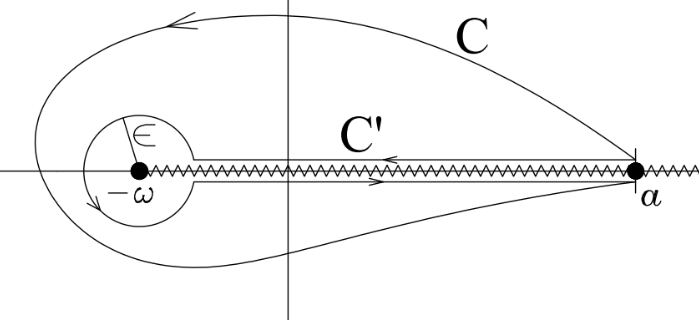
\includegraphics[width=.75\textwidth]{c32.PNG}
    \caption{The contour of integration with branch point at $-\omega$  and  branch  cut  runs  from $(-\omega,\infty)$.}
    \label{ch33}
\end{figure}

Lastly, to exactly evaluate the the generalized Stieltjes transform of the non-integral order
\begin{equation}\label{pf}
	S_{n+\alpha}^{a}[f(x)] = \int_{0}^{a}\frac{f(x)}{(\omega+x)^{n+\alpha}}\mathrm{d}x, 
\end{equation}
where $f(x)$ has an entire complex extension $f(z)$ and $\alpha$ is between $0$ and $1$. Again, we need to lift the integral to the complex plane. Doing so will induce a branch point at $z=-\omega$ and we choose that branch cut will run along the positive real axis. Now, consider a complex contour integral in the form of 
\begin{equation}
     \int_{C} \frac{f(z)}{(\omega + z)^{n+\alpha}} \mathrm{d}z ,
\end{equation}
where the contour $C$ is shown in the Figure \ref{ch33}. The contour will be deform to $C'$ and evaluating it will result to
\begin{eqnarray}\label{3.81}
\int_{C^\prime}\frac{f(z)}{(\omega+z)^{n+\alpha}}\mathrm{d}z&=&\int_a^{-\omega+\epsilon}\frac{f(x)}{(\omega+x)^{n+\alpha}}\mathrm{d}x + \int_{\epsilon}\frac{f(z)}{(\omega+z)^{n+\alpha}}\mathrm{d}z\nonumber\\\nonumber
&+&\int_{-\omega+\epsilon}^a\frac{f(x)}{(\omega+x)^{n+\alpha}e^{2\pi i(n+\alpha)}}\mathrm{d}x\\
&=&\int_a^{-\omega+\epsilon}\frac{f(x)}{(\omega+x)^{n+\alpha}}\mathrm{d}x+\int_{\epsilon}\frac{f(z)}{(\omega+z)^{n+\alpha}}\mathrm{d}z\\
 \quad & +&e^{-2\pi i\alpha}\int_{-\omega+\epsilon}^a\frac{f(x)}{(\omega+x)^{n+\alpha}}\mathrm{d}x\nonumber \\
&=&(e^{-2\pi i\alpha}-1)\int_{-\omega+\epsilon}^a\frac{f(x)}{(\omega+x)^{n+\alpha}}\mathrm{d}x+\int_{\epsilon}\frac{f(z)}{(\omega+z)^{n+\alpha}}\mathrm{d}z \nonumber
\end{eqnarray}
Combining the similar terms and using the parameterization $z = \epsilon\mathrm{e}^{i\theta}$, the resulting equation is
\begin{align}
\begin{split}
  \int_{C^\prime}\frac{f(z)}{(\omega+z)^{n+\alpha}}\mathrm{d}z &= (e^{-2\pi i\alpha}-1)\left [\int_{-\omega+\epsilon}^{0}\frac{f(x)}{(\omega+x)^{n+\alpha}}\mathrm{d}x+\int_{0}^{a}\frac{f(x)}{(\omega+x)^{n+\alpha}}\mathrm{d}x\right ]\\& \qquad +\int_{\epsilon}\frac{f(\epsilon \mathrm{e}^{i\theta} - \omega)}{(\epsilon \mathrm{e}^{i\theta})^{n+\alpha-1}}i\mathrm{d}\theta.
\end{split}
\end{align}
For the first term above, we will do a u-substitution technique. We will let $x = x' + \omega$, the first term will become
\begin{equation}
    \int_{-\omega+\epsilon}^{0}\frac{f(x)}{(\omega+x)^{n+\alpha}}\mathrm{d}x = \int_{\epsilon}^{\omega}\frac{f(x' - \omega)}{(x')^{n+\alpha}}\mathrm{d}x'.
\end{equation}
Dividing both sides by the factor $(e^{-2\pi i\alpha}-1)^{-1}$ and rearranging the terms such that we obtain the desired integral

\begin{align}
\begin{split}
 \int_0^a \frac{f(x)}{(\omega + x)^{n+\alpha}} \mathrm{d}x  & = \frac{1}{e^{-2\pi i\alpha}-1}\int_{C'}\frac{f(z)}{(\omega+z)^{n+\alpha}}\mathrm{d}z  
\\& \int_{\epsilon}^{\omega}\frac{f(x - \omega)}{(x)^{n+\alpha}}\mathrm{d}x -\frac{1}{e^{-2\pi i\alpha}-1} \int_{\epsilon}\frac{f(\epsilon \mathrm{e}^{i\theta} - \omega)}{(\epsilon \mathrm{e}^{i\theta})^{n+\alpha-1}}i\mathrm{d}\theta
\end{split}
\end{align}
To evaluate the the first term above, we will expand the binomial $(\omega+z)^{n+\alpha}$ with its binomial expansion at the origin given by
\begin{equation}
    \frac{1}{(\omega+z)^{n+\alpha}} = \sum_{k=0}^{\infty} {n+\alpha \choose k} \frac{\omega^{k}}{z^k+n+\alpha}
\end{equation}
Inserting this binomial expansion to the first term will give us
\begin{align}
\begin{split}
    \frac{1}{e^{-2\pi i\alpha}-1}\int_{C'}\frac{f(z)}{(\omega+z)^{n+\alpha}}\mathrm{d}z & =  \frac{1}{e^{-2\pi i\alpha}-1}\int_{C}\sum_{k=0}^{\infty} {n+\alpha \choose k} \omega^{k}\frac{f(z)}{(z)^{k+n+\alpha}}\mathrm{d}z \\& = \sum_{k=0}^{\infty} {n+\alpha \choose k} \omega^{k}  \frac{1}{e^{-2\pi i\alpha}-1}\int_{C} \frac{f(z)}{(z)^{k+n+\alpha}}\mathrm{d}z .
\end{split}
\end{align}
Again, similar to the previous section, the interchanging of order of the integration and summation is valid since the expansion and the contour is uniformly convergent for all $|z| > b$. It can also be shown formally by establishing a constant bound for the finite-part integral, by deforming the contour to a circle with radius a. Similar to the other section, it can established that the series is absolutely convergent for $\omega < a$. Now, invoking Theorem \ref{T3.2} the contour integral becomes
\begin{equation}
     \frac{1}{e^{-2\pi i\alpha}-1}\int_{C'}\frac{f(z)}{(\omega+z)^{n+\alpha}}\mathrm{d}z=\sum_{k=0}^{\infty} {n+\alpha \choose k} \omega^{k} \bbint{0}{a} \frac{f(z)}{(z)^{k+n+\alpha}}\mathrm{d}z 
\end{equation}
For the remaining terms which is dependent of $\epsilon$. It can be recognized that those terms is divergent at the origin. Lifting it to the contour integral and by the virtue of Theorem \ref{T3.2}, it will result to a finite-part integration
\begin{equation}
\bbint{0}{\omega}\frac{f(x-\omega)}{(x)^{n+\alpha}}\mathrm{d}x=\lim_{\epsilon\rightarrow0}\left[\int_{0}^{\omega-\epsilon}\frac{f(-x)}{(\omega-x)^{n+\alpha}}\mathrm{d}x-\frac{1}{e^{-2\pi i\alpha}-1} \int_{\epsilon}\frac{f(\epsilon \mathrm{e}^{i\theta} - \omega)}{(\epsilon \mathrm{e}^{i\theta})^{n+\alpha-1}}i\mathrm{d}\theta \right]
\end{equation}
Finally, we obtain a representation of the given integral presented in equation \eqref{pf} in terms of two finite part integral,
\begin{equation}\label{new}
\int_{0}^{a}\frac{f(x)}{(\omega+x)^{n+\alpha}}\mathrm{d}x=\sum_{k=0}^{\infty} {n+\alpha \choose k} \omega^{k} \bbint{0}{a} \frac{f(z)}{(z)^{k+n+\alpha}}\mathrm{d}z -\bbint{0}{\omega}\frac{f(x-\omega)}{x^{n+\alpha}}\mathrm{d}x.
\end{equation}
The finite-part integral arises from the singularity of the kernel of transformation will be called the progenic finite-part integrals. Evaluating further this progenic finite-part integrals, will result to
\begin{align}
\begin{split}
	\Delta_{\mathrm{sc}}^{(n+\alpha)} & (\omega) = \bbint{0}{\omega}\frac{f(x-\omega)}{x^{n+\alpha}}\mathrm{d}x
	\\& \quad= \sum_{j=0}^{\infty}\frac{f^{\left(j\right)}\left(-\omega\right) \,\omega^{j-n-\alpha+1}}{j!\,\left(j-n-\alpha+1\right)} .
\end{split}
\end{align}
The two equations above reproduce the theorem that can be found in \cite{tica2019finite}
\begin{theorem}\label{T3.5}
	Let $f(x)$ be locally integrable in the interval $[0,a]$ with an entire complex extension $f(z)$. Then
	\begin{equation}\label{new_rezult}
	\int_0^a\frac{f(x)}{(\omega+x)^{n+\alpha}}\mathrm{d}x=\sum_{j=0}^{\infty}{{-n-\alpha}\choose {j}}\, {\omega}^j \, \bbint{0}{a}\frac{f(x)}{x^{n+\alpha+j}}\mathrm{d}x + \Delta_{\mathrm{sc}}^{(n+\alpha)}(\omega),
	\end{equation}
	where $n=1,2,3...$ and $0<\alpha<1$, provided $\omega<a$, in which the singular contribution is the finite part integral
	\begin{align}
    \begin{split}\label{3.79}
	\Delta_{\mathrm{sc}}^{(n+\alpha)} & (\omega) =- \bbint{0}{\omega} \frac{f(-x)}{(\omega-x)^{n+\alpha}}\mathrm{d}x
	\\& \quad= \sum_{j=0}^{\infty}\frac{f^{\left(j\right)}\left(-\omega\right) \,\omega^{j-n-\alpha+1}}{j!\,\left(j-n-\alpha+1\right)} .
	\end{split}
    \end{align}
\end{theorem}

\section{Finite-part Integration in the Presence of Competing Singularities}

Now, we already see how the method is implemented to evaluate the Stieltjes transform. The theorems for the exact evaluation of the Stieltjes transform are only established for the functions with an entire complex extension. Recent development of the method is the application of finite-part integration to the Stieltjes transform of a function $f(x)$ with competing singularities when lifted to a complex plane.

According to \cite{doi:10.1063/5.0038274, lloydthetit}, the theorems presented from the previous section will still hold regardless of the nature of singularities that the complex extension of $f(x)$ possess, provided with some restriction. The first restriction comes from the desire to represent the contour integral as a finite-part integral. According to the conditions imposed by Theorem \ref{T3.1} and \ref{T3.2}, the contour should not enclose any singularities of $f(z)$. Also, it is specific that the contour $C$ should traverse the positive real axis of the complex plane as shown in Figure \ref{ch31}. Those conditions limit the possible choices of the complex extension of the function $f(z)$. For example, if $f(z)$ has a pole, then the pole must be located on the left-hand side of the complex plane since your contour is straddling along the positive real axis. Additionally, the branch cut of $f(z)$ should not overlap with the branch cut from the complex extension of the kernel of the transformation $(\omega + z)^{k+\nu}$. The second restriction comes from the method itself. Recall that to recover the missing terms from the term by term integration, the method requires the contour $C$ to enclose the singularity of the kernel located at $z=-\omega$. This requires the $\omega$ to be located not farther from the origin compared to the nearest singularity of $f(z)$. This implies that the radius of convergence of the infinite series in the right-hand side of the Theorems \ref{T3.3}, \ref{T3.4}, and $\ref{T3.5}$ is less than the distance of the nearest singularity of $f(z)$ with respect to the origin. Thus, the presence of singularities of $f(z)$ create a restriction on the radius of convergence of the infinite series of the finite-part integrals.

To appreciate it further, we will apply the method to the generalized Stietljes transform of $f(x) = (a+x)^{-\mu}$, which will have a singularity at $-a$. 

\subsection{Finite-part integration of the generalized Stieltjes transform of non-integral order}
In this case, we will evaluate the generalized Stieltjes transform of $f(x) = (a+x)^{-\mu}$ with non-integral order
\begin{equation}
    S_{m+\nu}[(a+x)^{-\mu}] = \int_{0}^{\infty} \frac{(a+x)^{-\mu}}{(\omega+x)^{m+\nu}} \mathrm{d}x, \quad 0<\nu<1.
\end{equation}
The divergence will be caused by the branch point singularity when the kernel expands at the origin. Moreover, when the integral is lifted to the complex plane, we will have a branch point singularity at $z=-\omega$ due to the kernel. We choose the branch cut to run along the positive real axis. Therefore, to solve the integral, we will consider the contour integral
\begin{equation}
    \int_{C} \frac{(a+z)^{-\mu}}{(\omega+z)^{m+\nu}} \mathrm{d}z.
\end{equation}

 \begin{figure}[t]
 	\centering
 	\includegraphics[width=0.75\textwidth]{c21.PNG}
 	 	\includegraphics[width=0.75\textwidth]{c12.PNG}
 	\caption{The deformation of the contour $\mathrm{C}$ to the contour $\mathrm{C}'$ to extract the Stieltjes integral. (Top) The point $z=-\omega$ is a branch point of the kernel transformation. (Bottom) The point $z=-\omega$ is a pole of the kernel of transformation. The point $z=-\tau$ is a branch point or a pole of the complex extension $f(z)$ of the function $f(x)$.}
 	\label{deformation}
 \end{figure}

The figure for the contour is obtained from \cite{doi:10.1063/5.0038274}.The top figure in Figure \ref{deformation} is the contour for the above expression. It is noticeable that the contour avoids the singularity of the function $f(z)$ or chosen to be far away from the origin, i.e., $a > \omega$. This translates to $\mu$ can be any positive number, or the nature of singularity of $f(z)$ would not matter. Deforming the contour to $C'$ as shown in the Figure \ref{deformation} and evaluate it, we will have
\begin{align}
\begin{split}
    \int_{C'} \frac{(a+z)^{-\mu}}{(\omega+z)^{m+\nu}}\,& \,\mathrm{d}z 
    = \left( e^{-2\pi i \nu}-1 \right) \int_{-\omega+\epsilon}^{\infty} \frac{ (a+x)^{-\mu}}{(b+x)^{m+\nu}} \, \mathrm{d}x 
    \\& + \int_{\epsilon} \frac{(a-\omega+\epsilon \mathrm{e}^{i\theta})^{-\mu}}{(\epsilon \mathrm{e}^{i\theta})^{m+\nu-1}}\, i \mathrm{d}\theta.
\end{split}
\end{align}
Recovering the Stietljes integral by rearranging the terms, and dividing both sides by $\left( e^{-2\pi i \nu}-1 \right)$, we will have
\begin{align}
\begin{split}
    \int_{0}^{\infty} \frac{ (a+x)^{-\mu}}{(b+x)^{m+\nu}} \, \mathrm{d}x  =  & \frac{1}{\left( e^{-2\pi i \nu}-1 \right)} \int_{C'} \frac{(a+z)^{-\mu}}{(\omega+z)^{m+\nu}} \,\mathrm{d}z \\& - \int_{-\omega+\epsilon}^{0} \frac{ (a+x)^{-\mu}}{(b+x)^{m+\nu}} \, \mathrm{d}x \\&  - \frac{1}{\left( e^{-2\pi i \nu}-1 \right)} \int_{\epsilon} \frac{(a-\omega+\epsilon \mathrm{e}^{i\theta})^{-\mu}}{(\epsilon \mathrm{e}^{i\theta})^{m+\nu-1}}\, i \mathrm{d}\theta.
\end{split}
\end{align}
Next, expanding the kernel of the contour integral at the origin and identify it as a finite-part integral using Theorem \ref{T3.1} will result to 
\begin{align}
\begin{split}
    \int_{0}^{\infty} \frac{ (a+x)^{-\mu}}{(\omega+x)^{m+\nu}} \, \mathrm{d}x  =  & \sum_{k=0}^{\infty} \binom{-m-\nu}{k} \omega^{k} \bbint{0}{\infty} \frac{(a+z)^{-\mu}}{z^{k+m+\nu}} \\& - \int_{-\omega+\epsilon}^{0} \frac{ (a+x)^{-\mu}}{(\omega+x)^{m+\nu}} \, \mathrm{d}x \\&  - \frac{1}{\left( e^{-2\pi i \nu}-1 \right)} \int_{\epsilon} \frac{(a-\omega+\epsilon \mathrm{e}^{i\theta})^{-\mu}}{(\epsilon \mathrm{e}^{i\theta})^{m+\nu-1}}\, i \mathrm{d}\theta.
\end{split}
\end{align}
For the remaining terms, we will perform a u-substitution $u = x+\omega$, and we will take the limit of $\epsilon \to 0$
\begin{align}
\begin{split}
    \int_{0}^{\infty} \frac{ (a+x)^{-\mu}}{(\omega+x)^{m+\nu}} \, \mathrm{d}x  =  & \sum_{k=0}^{\infty} \binom{-m-\nu}{k} \omega^{k} \bbint{0}{\infty} \frac{(a+z)^{-\mu}}{z^{k+m+\nu}} \\& - \lim_{\epsilon \to 0} \, \Bigg[ \int_{\epsilon}^{\omega} \frac{ (a-\omega+u)^{-\mu}}{u^{m+\nu}} \, \mathrm{d}u \\&  - \frac{1}{\left( e^{-2\pi i \nu}-1 \right)} \int_{\epsilon} \frac{(a-\omega+\epsilon \mathrm{e}^{i\theta})^{-\mu}}{(\epsilon \mathrm{e}^{i\theta})^{m+\nu-1}}\, i \mathrm{d}\theta \Bigg].
\end{split}
\end{align}
The remaining terms can be recognized that those terms are divergent at the origin. Lifting it to the contour integral and by virtue of Theorem \ref{T3.2}, it will result in a finite-part integration
\begin{align}
\begin{split}
\bbint{0}{\omega}\frac{f(x-\omega)}{x^{n+\alpha}}\,&\mathrm{d}x=\lim_{\epsilon\rightarrow0}\Bigg[\int_{0}^{\omega-\epsilon}\frac{f(-x)}{(\omega-x)^{n+\alpha}}\mathrm{d}x \\& \quad-\frac{1}{e^{-2\pi i\alpha}-1} \int_{\epsilon}\frac{f(\epsilon \mathrm{e}^{i\theta} - \omega)}{(\epsilon \mathrm{e}^{i\theta})^{n+\alpha-1}}i\mathrm{d}\theta \Bigg].
\end{split}
\end{align}
Finally, collecting all the results, we expressed the Stieltjes transform as a finite-part integral
\begin{align}
\begin{split}
    \int_{0}^{\infty} \frac{ (a+x)^{-\mu}}{(\omega+x)^{m+\nu}} \, \mathrm{d}x  =  & \sum_{k=0}^{\infty} \binom{-m-\nu}{k} \omega^{k} \bbint{0}{\infty} \frac{(a+z)^{-\mu}}{z^{k+m+\nu}} \\& - \bbint{0}{\omega} \frac{(a-\omega+x)^{-\mu}}{x^{m+\nu}}.
    \label{c2I1}
\end{split}
\end{align}
Obviously, the above equation can be obtained easily using theorem \ref{T3.5}. This confirmed the applicability of the theorem for the function with competing singularities.

To evaluate the first finite-part integral, we will consider it first as a usual integral with the bounds $\epsilon$ to $c$. We will determine the nature of each term (converging and diverging) at the limit $\epsilon \to 0$. to obtain the finite part value, we will drop the terms that will diverge and retain the converging terms. Lastly, we will evaluate the limit $c \to \infty$  to obtain the desired finite-part integral. 

Now, consider the finite-part integral as a usual integral with bounds $\epsilon$ and $c$. Then, we expand the $f(x)$ at the origin using the Taylor series expansion. The process will result to
\begin{equation}
    \int_{\epsilon}^{c}  \frac{(a+x)^{-\mu}}{x^{k+m+\nu}} \, \mathrm{d}x =  \int_{\epsilon}^{c} \sum_{l=0}^{\infty} \binom{-\mu}{l} \frac{1}{a^{k+\mu}} x^{l-k-m-\nu} \, \mathrm{d}x.
\end{equation}
The infinite series is absolutely convergence for $|x/a| < 1$. The convergence will permit the interchanging of the order of summation and integration. Performing a term by term integration, which will results to
\begin{equation}
    \int_{\epsilon}^{c}  \frac{(a+x)^{-\mu}}{x^{k+m+\nu}} \, \mathrm{d}x = \sum_{l=0}^{\infty} \binom{-\mu}{l} \frac{1}{a^{k+\mu}} \left. \frac{x^{l-k-m-\nu+1}}{l-k-m-\nu+1} \right|_{\epsilon}^{c}.
\end{equation}
Again, we can group the terms by taking the limits $\epsilon \to 0$. The terms from $0$ to $k+m-1$ that have a factor of $\epsilon$ will have diverging terms when $\epsilon \to 0$ since all the terms have a negative exponent. The rest of the terms will converge.  Doing so, we will have
\begin{align}
\begin{split} 
    C_\epsilon = & \sum_{l=0}^{\infty} \binom{-\mu}{l} \frac{1}{a^{k+\mu}} \frac{c^{l-k-m-\nu+1}}{l-k-m-\nu+1} \\& \quad -  \sum_{l=k+m}^{\infty} \binom{-\mu}{l} \frac{1}{a^{k+\mu}} \frac{c^{l-k-m-\nu+1}}{l-k-m-\nu+1},
\end{split}
\end{align}
\begin{equation}
    D_\epsilon =- \sum_{l=0}^{k+m-1} \binom{-\mu}{l} \frac{1}{a^{k+\mu}}  \frac{\epsilon^{l-k-m-\nu+1}}{l-k-m-\nu+1}. 
\end{equation}

Taking the limits $\epsilon \to 0$ and dropping the diverging terms will lead us to the value of finite-part integral 
\begin{align}
\begin{split} 
    \bbint{0}{c} \frac{(a+x)^{-\mu}}{x^{k+m+\nu}} \, \mathrm{d}x = \sum_{l=0}^{\infty} \binom{-\mu}{l} \frac{1}{a^{k+\mu}} \frac{c^{l-k-m-\nu+1}}{l-k-m-\nu+1},
\end{split}
\end{align}
the terms of the convergent group with $\epsilon$ factor will vanish since it will just approach 0. Now, it's time to take the limit $c \to \infty$. This will make the terms with negative powers vanished since a factor of $1/c \to 0$ as $c \to \infty$,
\begin{align}
\begin{split} 
    \bbint{0}{\infty} \frac{(a+x)^{-\mu}}{x^{k+m+\nu}} \, \mathrm{d}x = \lim_{c \to \infty} \sum_{l=k+m}^{\infty} \binom{-\mu}{l} \frac{1}{a^{k+\mu}} \frac{c^{l-k-m-\nu+1}}{l-k-m-\nu+1}.
\end{split}
\end{align}
The evaluate the limits, we will convert the infinite series to the form of hypergeometric function express in equation \eqref{GHF} and will consider its asymptotic expansion at the very large argument. In expressing the series as a hypergeometric function, we first need to ensure that the interval of the series start at zero, if not, shifting of the interval is needed to perform. Also, the pochammer symbol \cite[pg. 3, Eq. 1.1.1.2]{slater1966generalized}
\begin{equation}
    (a)_k = \frac{\Gamma(k+a)}{a}
\end{equation}
and the negative binomial theorem \cite{nbt}
\begin{equation}
    \binom{-\mu}{n} = (-1)^{n} \binom{n+\mu-1}{n} = (-1)^{n} \frac{\Gamma(n+\mu)}{\Gamma(n+1)\Gamma(\mu)},
\end{equation}
were needed in the algebraic manipulation of the series. Rewriting the series into hypergeometric function will result to
\begin{align}
\begin{split} 
    \bbint{0}{\infty} \frac{(a+x)^{-\mu}}{x^{k+m+\nu}} \, \mathrm{d}x & = \lim_{c \to \infty} \sum_{l=0}^{\infty} \binom{-\mu}{l+k+m} \frac{1}{a^{l+k+m+\mu}} \frac{c^{l-\nu+1}}{l-\nu+1}
    \\& 
    = \lim_{c \to \infty} \sum_{l=0}^{\infty} \frac{(-1)^{l+k+m} \Gamma(l+k+m+\mu)}{\Gamma(\mu)\Gamma(l+k+m+1)} \frac{1}{a^{l+k+m+\mu}} \frac{c^{l-\nu+1}}{l-\nu+1}
    \\& = \lim_{c \to \infty}\frac{(-1)^{k+m} c^{1-\nu}}{a^{k+m+\mu}} \frac{\Gamma(k+m+\mu) \Gamma(1-\nu)}{\Gamma(\mu)\Gamma(k+m+1)\Gamma(2-\nu)}
    \\& \qquad \times \sum_{l=0}^{\infty} \frac{(1)_{k} (k+m+\mu)_{l}(1-\nu)^{l}}{(m+1)_l(2-\nu)_l} \frac{(-c/a)^{l}}{l!}
    \\& = \lim_{c \to \infty}\frac{(-1)^{k+m} c^{1-\nu}}{a^{k+m+\mu}} \frac{\Gamma(k+m+\mu) \Gamma(1-\nu)}{\Gamma(\mu)\Gamma(k+m+1)\Gamma(2-\nu)}
    \\& \qquad \times \pFq{3}{2}{1, k+m+\mu,1-\nu}{k+m+1,2-\nu}{-\frac{c}{a}}.
\end{split}
\end{align}
The asymptotic expansion of ${}_3F_2$ at the very large argument \cite{wolfram} is written as
\begin{align}
\begin{split}
   \,& \pFq{3}{2}{a_1,a_2,a_3}{b_1.b_2}{-z} =  \\& \quad \quad  \frac{\Gamma(b_1) \Gamma(b_2)}{\Gamma(a_1) \Gamma(a_2) \Gamma(a_3)}  \Bigg( \frac{\Gamma(a_1) \Gamma(a_2-a_1) \Gamma(a_3-a_1)}{\Gamma(b_1-a_1) \Gamma(b_2-a_1) \Gamma(a_3)} (-z)^{-a_1} \left(  1+\mathcal{O} \left( \frac{1}{z} \right) \right) \\& \quad \quad \quad + \frac{\Gamma(a_2) \Gamma(a_1-a_2) \Gamma(a_3-a_2)}{\Gamma(b_1-a_2) \Gamma(b_2-a_2) \Gamma(a_3)} (-z)^{-a_2} \left(  1+\mathcal{O} \left( \frac{1}{z} \right) \right) \\& \quad \quad \quad \quad +  \frac{\Gamma(a_3) \Gamma(a_1-a_3) \Gamma(a_2-a_3)}{\Gamma(b_1-a_3) \Gamma(b_2-a_3) \Gamma(a_3)} (-z)^{-a_3} \left(  1+\mathcal{O} \left( \frac{1}{z} \right) \right) \Bigg) ,  |z| \to \infty.
\label{3F2simple} 
\end{split}
\end{align}
Since we will let $c \to \infty$, only the $z$ term with exponent $1-\nu$ will have a contribution
\begin{align}
\begin{split} 
    \bbint{0}{\infty} \frac{(a+x)^{-\mu}}{x^{k+m+\nu}} \, \mathrm{d}x &  =\frac{(-1)^{k+m}}{a^{k+m+\mu}} \frac{\Gamma(1-\nu)\Gamma(\nu)\Gamma(k+m+\mu+\nu-1)}{\Gamma(\mu) \Gamma(k+m+\nu)}.
\end{split}
\end{align}
Using the reflection relation of Gamma function \cite[p. 58-59]{hardy1940ramaniyan}
\begin{equation}
    \Gamma(z)\Gamma(1-z) = \frac{\pi}{\sin{\pi z}},
\end{equation}
the finite-part integral simplifies to
\begin{align}
\begin{split} 
    \bbint{0}{\infty} \frac{(a+x)^{-\mu}}{x^{k+m+\nu}} \, \mathrm{d}x &  = \frac{(-1)^{k+m}}{a^{k+m+\mu}} \frac{\pi}{\sin{\pi\nu}} \frac{\Gamma(k+m+\mu+\nu-1)}{\Gamma(\mu) \Gamma(k+m+\nu)}.
\end{split}
\end{align}
For the finite-part integral of the singular contribution, we will just do the same process. However, in this case, we only need to take the limit $\epsilon \to 0$ and change the lower limit to $\epsilon$. The change in variable for the upper limit is not needed since $\omega$ is only finite. Now, consider it as a usual integral and perform an expansion
\begin{equation}
    \int_{\epsilon}^{\omega} \frac{(a-\omega+x)^{-\mu}}{x^{m+\nu}} \, \mathrm{d}x = \int_{\epsilon}^{\omega} \sum_{k=0}^{\infty} \frac{1}{(a-\omega)^{k+\mu}} x^{k-m-\nu} \, \mathrm{d}x.
\end{equation}
It is certain that the summation is convergent for $|z| < |a-\omega|$. Therefore, the interchanging of the operators and term by term integration is allowed
\begin{equation}
    \int_{\epsilon}^{\omega} \frac{(a-\omega+x)^{-\mu}}{x^{m+\nu}} \, \mathrm{d}x = \sum_{k=0}^{\infty} \binom{-\mu}{k} \frac{1}{(a-\omega)^{k+\mu}} \left.  \frac{x^{k-m-\nu+1}}{k-m-\nu+1} \right|_{\epsilon}^{\omega}.
\end{equation}
Now, grouping the terms into converging and diverging group, we will have
\begin{align}
\begin{split} 
    C_\epsilon = & \sum_{k=0}^{\infty} \binom{-\mu}{k} \frac{1}{(a-\omega)^{k+\mu}} \frac{\omega^{k-m-\nu+1}}{k-m-\nu+1} \\& \quad -  \sum_{k=m}^{\infty} \binom{-\mu}{k} \frac{1}{(a-\omega)^{k+\mu}} \frac{\epsilon^{k-m-\nu+1}}{k-m-\nu+1},
\end{split}
\end{align}
\begin{equation}
    D_\epsilon = -\sum_{k=0}^{m-1} \binom{-\mu}{k} \frac{1}{(a-\omega)^{k+\mu}}  \frac{\epsilon^{k-m-\nu+1}}{k-m-\nu+1}. 
\end{equation}
To obtain the finite-part integral, we will now take the limit of $\epsilon \to 0$ and drop the diverging group, this will result to
\begin{align}
\begin{split} 
    \bbint{0}{\omega} \frac{(a-\omega+x)^{-\mu}}{x^{m+\nu}} \, \mathrm{d}x = & \sum_{k=0}^{\infty} \binom{-\mu}{k} \frac{1}{(a-\omega)^{k+\mu}} \frac{\omega^{k-m-\nu+1}}{k-m-\nu+1}.
\end{split}
\end{align}
The above series can be express in the form of hypergeometric function express in equation \eqref{GHF}, doing so will give us
\begin{align}
\begin{split} 
    \bbint{0}{\omega} \frac{(a-\omega+x)^{-\mu}}{x^{m+\nu}} \, \mathrm{d}x & =  \sum_{k=0}^{\infty} \frac{(-1)^{k}\Gamma(k+\mu)}{\Gamma(\mu)k!}  \frac{1}{(a-\omega)^{k+\mu}} \frac{\omega^{k-m-\nu+1}}{k-m-\nu+1}
    \\& = \frac{\omega^{1-m-\nu}}{\Gamma(\mu) (1-m-\nu)} \sum_{k=0}^{\infty} \frac{(\mu)_{k}(1-m-\nu)_k}{(2-m-\nu)_k k!} \left(\frac{\omega}{\omega-a}\right)^{k}
    \\& = \frac{\omega^{1-m-\nu}}{\Gamma(\mu) (1-m-\nu)} \pFq{2}{1}{\mu,1-m-\nu}{2-m-\nu}{\frac{\omega}{\omega-a}}.
\end{split}
\end{align}
Collecting all the result and substituting back to equation \eqref{c2I1}, we will have
\begin{align}
\begin{split}
    \int_{0}^{\infty} & \frac{ (a+x)^{-\mu}}{(\omega+x)^{m+\nu}} \, \mathrm{d}x \\& = \sum_{k=0}^{\infty} \binom{-m-\nu}{k} \omega^{k} \frac{(-1)^{k+m}}{a^{k+m+\mu}} \frac{\pi}{\sin{\pi\nu}} \frac{\Gamma(k+m+\mu+\nu-1)}{\Gamma(\mu) \Gamma(k+m+\nu)}  \\& \quad - \frac{\omega^{1-m-\nu}}{\Gamma(\mu) (1-m-\nu)} \pFq{2}{1}{\mu,1-m-\nu}{2-m-\nu}{\frac{\omega}{\omega-a}}.
\end{split}
\end{align}
We see that the infinite series of the first term is only absolutely convergent for $|\omega/a| < 1$. This is the effect of the singularities from the function $f(z)$. It limits the convergence of the result of the method. To access the region of $|\omega/a| > 1$, we will resort to the concept of analytic continuation. Therefore, we need to close the series to invoke the principle of an analytic function and extend the analyticity to a larger region. Closing the series means expressing the series to a known elementary/special function. Fortunately, the series can be close using the hypergeometric function with a form written in equation \eqref{GHF}. Doing so, we will have
\begin{align}
\begin{split}
    \int_{0}^{\infty} & \frac{(a+x)^{-\mu}}{(\omega+x)^{m+\nu}} \, \mathrm{d}x \\& = \frac{\pi}{\sin{\pi\nu}} \sum_{k=0}^{\infty} \frac{(-1)^{k}\Gamma(k+\mu+\nu)}{\Gamma(m+\nu)k!} \omega^{k} \frac{(-1)^{k+m}}{a^{k+m+\mu}}  \frac{\Gamma(k+m+\mu+\nu-1)}{\Gamma(\mu) \Gamma(k+m+\nu)}  \\& \quad - \frac{\omega^{1-m-\nu}}{\Gamma(\mu) (1-m-\nu)} \pFq{2}{1}{\mu,1-m-\nu}{2-m-\nu}{\frac{\omega}{\omega-a}}.
    \\&= \frac{\pi}{\sin{\pi\nu}} \frac{(-1)^{m} \Gamma(m+\mu+\nu-1)}{\Gamma(\mu) \Gamma(m+\nu)a^{m+\mu}} \sum_{k=0}^{\infty}  \frac{(m+\mu+\nu-1)_{k} (\omega/a)^{k}}{k!}  \\& \quad - \frac{\omega^{1-m-\nu}}{\Gamma(\mu) (1-m-\nu)} \pFq{2}{1}{\mu,1-m-\nu}{2-m-\nu}{\frac{\omega}{\omega-a}}.
\end{split}
\end{align}
Finally, we successfully evaluate the Stieltjes transform of $(a-x)^{-\mu}$ of non-integral order
\begin{align}
\begin{split}
    \int_{0}^{\infty} & \frac{(a+x)^{-\mu}}{(\omega+x)^{m+\nu}} \, \mathrm{d}x \\& = \frac{\pi}{\sin{\pi\nu}} \frac{(-1)^{m} \Gamma(m+\mu+\nu-1)}{\Gamma(\mu) \Gamma(m+\nu)a^{m+\mu}} \pFq{1}{0}{m+\mu+\nu-1}{-}{\frac{\omega}{a}}  \\& \quad - \frac{\omega^{1-m-\nu}}{\Gamma(\mu) (1-m-\nu)} \pFq{2}{1}{\mu,1-m-\nu}{2-m-\nu}{\frac{\omega}{\omega-a}}.
\end{split}
\end{align}
The above result was already presented in \cite{Villanueva_Galapon_2019}.

We can see here the necessity to close the infinite series to access the region $a < \omega$ that restricts by the singularity of the complex extension of $f(x)$.

%%%%%%%%%%%%%%%%%%%%%%%%%%%%%%%%%%%%%%%%%%%%%%%%%%%%%%%%%%%%%%%%%%%%

\subsection{Finite-part integration of the generalized Stieltjes transform of integral order}
Lastly, we will consider the integral order of the generalized Stieltjes transform of $f(x) = (a+x)^{-\mu}$
\begin{equation}
    S_{m}[(a+x)^{-\mu}] = \int_{0}^{\infty} \frac{(a+x)^{-\mu}}{(\omega+x)^{m}} \mathrm{d}x.
\end{equation}
If we naively expand the kernel at the origin, the divergence is caused by the pole singularity. Also, the singularity due to the kernel is a pole singularity. With that, we need to induce a branch cut that runs along the positive real axis, and it can be induced by the complex extension of $\log x$. From that, we will consider the contour integral 
\begin{equation}
    \int_C \frac{(a+z)^{-\mu}}{(\omega +z )^{m}} \log{z} \, \mathrm{d}z,
\end{equation}
where the contour is the bottom figure of Figure \ref{deformation}. From the chosen contour, where we avoid the singularity of $f(z)$, we see that we pick $a$ to be very far away from the origin or at least $|a| > |\omega|$. In this condition, the nature of singularity of $f(z)$ would not matter. 

Similar to previous example, we will evaluate the deformed contour and extract the Stieltjes transform we want to evaluate
\begin{align}
\begin{split}
    \int_0^\infty \frac{(a+x)^{-\mu}}{(\omega+x)^m} \, \mathrm{d}x & = \frac{1}{2 \pi i} \int_C \frac{(a+z)^{-\mu}}{(\omega + z)^{m}} \, \left[ \log(z) -\pi i \right]\mathrm{d}z \\& \qquad - \mathrm{Res} \left[ \frac{ (a+z)^{-\mu}}{(\omega+z)^{m}}\, (\log(z) - \pi i)\right]_{z=-\omega}.
\end{split}
\end{align}
Expanding the kernel in the contour integral and we can express it as a finite-part integral by the virtue of Theorem \ref{T3.1}., we will have
\begin{align}
\begin{split}
    \int_0^\infty \frac{(a+x)^{-\mu}}{(\omega+x)^m} \, \mathrm{d}x & = \sum_{k=0}^{\infty} {-m \choose k} b^{k}   \bbint{0}{\infty} \frac{(a+x)^{-\mu}}{x^{k+m}} \mathrm{d}x \\& \qquad - \mathrm{Res} \left[ \frac{ (a+z)^{-\mu}}{(\omega+z)^{m}}\, (\log(z) - \pi i)\right]_{z=-\omega}.
\end{split}
\end{align}


Also, using equation \eqref{Res} we can easily evaluate the residue
\begin{align}
\begin{split} \label{SC}
    \mathrm{Res} \left[ \frac{(a+z)^{-\mu}}{(\omega+z)^{m}}\, \log(-z)\right]_{z=-\omega} = \,& \frac{(2-\mu-m)_{m-1}}{\Gamma(m) \, (a-\omega)^{\mu+m-1}} \, \log (\omega) \\& \hspace{-40mm} + \sum_{k=1}^{m-1} {m-1 \choose k} \frac{(-1)^k \Gamma(k)}{\omega^k} \frac{(2-\mu-m+k)_{m-1-k}}{(a-\omega)^{\mu+m-k-1}}.
\end{split}
\end{align}

Now, we will evaluate the finite-part integral. Again, we change its limit and treat it as a usual integral. Moreover, we expand the $(a+x)^{-\mu}$ with the convergence $|x/a|<1$ and interchange the order of summation and integration
\begin{equation}
    \int_{\epsilon}^{c} \frac{(a+x)^{-\mu}}{x^{k+m}} \, \mathrm{d}x = \sum_{l=0}^{\infty} \binom{-\mu}{l} \frac{1}{a^{l+\mu}} \int_{\epsilon}^{c} x^{l-k-m} \, \mathrm{d}x.
\end{equation}
Similar to the previous example, the interchanging of operators is allowed by the convergence of the series. Next, we will group the terms depending if they will converge or diverge when the limit $\epsilon \to 0$ is taken. For sure, negative integers of $\epsilon$ will diverge, which can be found in the interval $0 \leq l \leq k+m-2$. The term $l = k+m-1$ will also converge as $\epsilon \to 0$ since this is evaluated as a logarithm. Therefore, the groups are
\begin{align}
\begin{split} 
    C_\epsilon = & \sum_{l=k-m-2}^{\infty} \binom{-\mu}{l} \frac{1}{a^{k+\mu}} \frac{c^{l-k-m+1}}{l-k-m+1} + \binom{-\mu}{k+m-1} \frac{\ln{c}}{a^{k+m-1+\mu}} \\& \quad +\sum_{l=k-m}^{\infty} \binom{-\mu}{l} \frac{1}{a^{k+\mu}} \frac{c^{l-k-m+1}}{l-k-m+1} \\& \quad  -  \sum_{l=k+m}^{\infty} \binom{-\mu}{l} \frac{1}{a^{l+\mu}} \frac{\epsilon^{l-k-m-\nu+1}}{l-k-m-\nu+1},
\end{split}
\end{align}
\begin{align}
\begin{split} 
    D_\epsilon & = - \binom{-\mu}{k+m-1} \frac{\ln{\epsilon}}{a^{k+m-1+\mu}} \\& \qquad - \sum_{l=0}^{k+m-2} \binom{-\mu}{l} \frac{1}{a^{l+\mu}}  \frac{\epsilon^{l-k-m+1}}{l-k-m+1}. 
\end{split}
\end{align}
To obtain the finite-part integral, we will take the limit $\epsilon \to 0$ and disregard the diverging part. The $\epsilon$ with positive exponent will just approach zero
\begin{align}
\begin{split} 
    \bbint{0}{c} & \frac{(a+x)^{-\mu}}{x^{k+m}} \, \mathrm{d}x =  \sum_{l=0}^{k-m-2} \binom{-\mu}{l} \frac{1}{a^{l+\mu}} \frac{c^{l-k-m+1}}{l-k-m+1} \\& \quad + \binom{-\mu}{k+m-1} \frac{\ln{c}}{a^{k+m-1+\mu}}  +\sum_{l=k-m}^{\infty} \binom{-\mu}{l} \frac{1}{a^{l+\mu}} \frac{c^{l-k-m+1}}{l-k-m+1}
\end{split}
\end{align}
Now we take the limit $c \to \infty$, the terms with negative exponents will just vanish when evaluated. 
\begin{align}
\begin{split} \label{F1}
    \bbint{0}{\infty} \frac{(a+x)^{-\mu}}{x^{k+m}} \, \mathrm{d}x =  \lim_{c \to \infty} & \Bigg[ \sum_{l=k+m}^{\infty} \binom{-\mu}{l} \frac{1}{a^{l+\mu}} \frac{c^{l-k-m+1}}{l-k-m+1} \\& \qquad + \binom{-\mu}{k+m-1} \frac{\ln{c}}{a^{k+m-1+\mu}} \Bigg].
\end{split}
\end{align}
To evaluate the limits, we will obtain the closed form expression of the series, which is a hypergeometric function found in equation \eqref{GHF} 
\begin{align}
\begin{split} 
    \sum_{l=k+m}^{\infty} & \binom{-\mu}{l}  \frac{1}{a^{l+\mu}} \frac{c^{l-k-m+1}}{l-k-m+1} 
    \\&  = \sum_{l=0}^{\infty} \binom{-\mu}{l+k+m} \frac{1}{a^{l+k+m+\mu}} \frac{c^{l+1}}{l+1} 
    \\&  = \frac{c}{a^{k+m+\mu}} \sum_{l=0}^{\infty} \frac{(-1)^{l+k+m}\Gamma(l+k+m+\mu)}{\Gamma(\mu)\Gamma(l+k+m+1)(l+1)} \left(\frac{c}{a}\right)^{l} 
    \\& = \frac{(-1)^{k+m}c^{-1}}{a^{k+m+\mu}\Gamma(\mu)} \frac{\Gamma(k+m+\mu)}{\Gamma(k+m+1)} \sum_{l=0}^{\infty}  \frac{ (1)_{l} (1)_{l} (k+m+\mu)_l }{(k+m+1)_l (2)_l l!} \left(\frac{-c}{a}\right)^{l} 
    \\& = \frac{(-1)^{k+m}c^{-1}}{a^{k+m+\mu}\Gamma(\mu)} \frac{\Gamma(k+m+\mu)}{\Gamma(k+m+1)} \pFq{3}{2}{1,1,k+m+\mu}{2, k+m+1}{\frac{-c}{a}},
\end{split}
\end{align}
and use its asymptotic expansion at very large argument. The asymptotic expansion of ${}_3 F_2$ with a double pole for a large argument is given by
\begin{align}
\begin{split} \label{3F2doublepole}
    \,& \pFq{3}{2}{a_1,a_1,a_2}{b_1,b_2}{-z}   = \frac{\Gamma(b_1) \Gamma(b_2) \Gamma^2(a_1-a_3)} {\Gamma^2(a_1) \Gamma(b_1-a_3) \Gamma(b_2-a_3)} (-z)^{-a_3} \left( 1+\mathcal{O} \left( \frac{1}{z} \right) \right) \\& \quad + \frac{\Gamma(b_1) \Gamma(b_2) \Gamma(a_3-a_1)}{\Gamma(a_1) \Gamma(a_3) \Gamma(b_1-a_1) \Gamma(b_2-a_1)}  (\log(-z)+\psi(a_3-a_1)-\psi(b_1-a_1) \\& \quad \quad -\psi(b_2-a_1)-\psi(a_1)-2\gamma) (-z)^{-a_1} \left( 1+\mathcal{O} \left( \frac{1}{z} \right) \right), |z| \to \infty
\end{split} 
\end{align}
where $\psi(x)$ is a digamma function and $\psi(1) = -\gamma$ is the Euler-Masheroni constant \cite{wolfram1}. The first term will vanished since your $c$ will have a negative exponent, thus will approach to zero. Your second term will only contribute as $c \to \infty$ since the $c$ will cancel out
\begin{align}
\begin{split} 
    \sum_{l=k+m}^{\infty} & \binom{-\mu}{l}  \frac{1}{a^{l+\mu}} \frac{c^{l-k-m+1}}{l-k-m+1} 
    \\& = \frac{(-1)^{k+m}c^{-1}}{a^{k+m+\mu-1}\Gamma(\mu)}  \frac{\Gamma(1-k-m-\mu)}{\Gamma(k+m)} 
    \\& \qquad \times (\ln{(c/a)} + \psi(k+m+\mu-1) - \psi(k+m)).
\end{split}
\end{align}
Also, bringing  back the above equation to equation \eqref{F1}, the $\ln{c}$ will cancel out. The resulting finite-part integral is 
\begin{align}
\begin{split} 
    \bbint{0}{\infty} \frac{(a+x)^{-\mu}}{x^{k+m}} \,& \mathrm{d}x = \frac{1}{a^{k+m+\mu-1}}{-\mu \choose k+m-1} \\& \times \left(\ln(a) + \psi(k+m) - \psi(k+m+\mu-1) \right).
\label{FPIfinal}
\end{split}
\end{align}
Combining all the results, we will obtain 
\begin{align}
\begin{split} \label{22}
    &  \int_0^\infty \frac{(a+x)^{-\mu}}{(\omega+x)^m} \, \mathrm{d}x  = \sum_{k=0}^{\infty} {-\rho \choose k} \left( \frac{b}{a} \right)^{k} \frac{1}{a^{\rho+\mu-1}}{-\mu \choose k+\rho-1} \\&  \hspace{20 mm}\times \left(\log(a) + \psi(k+\rho) - \psi(k+\rho+\mu-1) \right) \\& - \left[ \frac{(2-\mu-\rho)_{\rho-1}}{\Gamma(\rho) \, (a-b)^{\mu+\rho-1}} \, \ln (b) - \sum_{k=1}^{\rho-1} {\rho-1 \choose k} \frac{ \Gamma(k)}{b^k} \frac{(2-\mu-\rho+k)_{\rho-1-k}}{(a-b)^{\mu+\rho-k-1}} \right].
\end{split}
\end{align}
Using binomial expansion on $(a-b)^{\mu+\rho-1}$ the coefficient of $\ln{b}$, we can readily see that the it is equal to the coefficient of $\ln{a}$. Therefore, we can combine the two terms leading the expression
\begin{align}
\begin{split}
    &  \int_0^\infty \frac{(a+x)^{-\mu}}{(\omega+x)^m} \, \mathrm{d}x  = \sum_{k=0}^{\infty} {-\rho \choose k} \left( \frac{b}{a} \right)^{k} \frac{1}{a^{\rho+\mu-1}}{-\mu \choose k+\rho-1} \\&  \hspace{20 mm}\times \left(\log(a)+ \psi(k+\rho) - \psi(k+\rho+\mu-1) \right) \\& - \left[ \frac{(2-\mu-\rho)_{\rho-1}}{\Gamma(\rho) \, (a-b)^{\mu+\rho-1}} \, \ln {\frac{b}{a}} - \sum_{k=1}^{\rho-1} {\rho-1 \choose k} \frac{ \Gamma(k)}{b^k} \frac{(2-\mu-\rho+k)_{\rho-1-k}}{(a-b)^{\mu+\rho-k-1}} \right].
\end{split}
\end{align}
The infinite series from the evaluated finite-part integration is again only convergent for $|b/a| < 1$. It is necessary to obtain a close form of this summation to access the region outside the convergence. This summation of the digamma function is expected to arise naturally in calculating the finite-part integral for the pole singularity case since we are most of the time using the double pole case of the asymptotic expansion of ${}_3F_2$. Therefore, it is necessary to study this hypergeometric-type series containing a digamma function as a factor.
\chapter{Hypergeometric-type Series Containing Digamma Function}
\label{ch_4}

This chapter will focus on the properties and behavior of the hypergeometric-type series containing a digamma function as a factor. From the previous chapter, we see how this type of series naturally appears in the calculation of the finite-part integration. There are already few papers that got interested in this type of series. The series was first tabulated in \cite{hansen1975table} but still there remains a significant gap. The exploitation of this series to produce a reduction formula of the Kampé de Fériet function can be seen in \cite{miller2006summations} and \cite{cvijovic2008closed}.

The chapter will start on the definition of hypergeometric-type series containing a digamma function as a factor. Next, we will establish its convergence and singularity. Then, if not defined on the whole complex plane, we will implement the concept of analytic continuation to extend the region of its analyticity. The goal is to find a representation of the series that will cover the whole complex plane and broaden the restrictions of each parameter. Lastly, we will derive the relation of this generalized series to the Kampé de Fériet function.

\section{Definitions}
The series 
\begin{align}
\begin{split}
      \psi(c) & + \frac{a_1 a_2 \dots a_p}{b_1 b_2 \dots b_q} \psi(c+1) \frac{z}{1!} \\& + \frac{a_1(a_1+1) a_2(a_2+1) \dots  a_p(a_p+1)}{b_1(b_1+1) b_2 (b_2+1) \dots b_q(b_q+1)} \psi(c+2) \frac{z^{2}}{2!} + \dots \\& \hspace{40mm} = \sum_{k=0}^{\infty} \frac{\prod_{l=1}^{p} (a_{l})_k}{ \prod_{l=1}^{q} (b_{l})_k} \psi(k+c) \frac{z^k}{k!}.
\end{split}
\end{align}
is a hypergeometric-type series containing a digamma function as a factor. It has a parameter of $\Vec{a}$, $\Vec{b}$, $c$, and $z$. Take note that $\Vec{a}$ means $a_1, a_2, \dots, a_p$ and $\Vec{b}$ corresponds to $b_1, b_2, \dots, b_q$. Any of these quantities may be real or complex. However, the parameter $\Vec{b}$ and $c$ must not be negative integers since they will make the series undefined. In addition, if any of the $a$ parameters is a negative integer, the function will reduce to a polynomial.  If the sum of the series exists, it will be denoted by the symbol 
\begin{equation}
    \pPq{p}{q}{\Vec{a}}{\Vec{b}}{c}{z}.
\end{equation}
Finally, we define the function $_{p}\tilde{\psi}_{q}$ with series representation of
\begin{equation} \label{psi}
    \pPq{p}{q}{\Vec{a}}{\Vec{b}}{c}{z} =  \sum_{k=0}^{\infty} \frac{\prod_{l=1}^{p} (a_{l})_k}{ \prod_{l=1}^{q} (b_{l})_k} \psi(k+c) \frac{z^k}{k!}.
\end{equation}
Obviously, the function $_{p}\tilde{\psi}_{q}$ is an analytic function since it is defined as a power series whenever the series converges.

\section{Convergence of the general series}

In studying an infinite series, the first thing we are interested in is its convergence. There are a lot of existing tests to tell if the series will diverge or converge. Most of the known tests can be found in \cite{hardy2018course}.

In general, a complex power series $\sum^{\infty} a_k z^k$ is said to converge only for certain values of $z$. This region is an open disk with radius $R$, where the number $R$ is called the radius of convergence. The power series will always converge absolutely for all the values of $z$ inside the open disk and will diverge outside it. On the boundary of the disk, the behavior of the power series is said to be complicated since it may converge or diverge \cite{hardy1940ramaniyan}. Therefore, it is important to determine the number $R$ or the radius of convergence to establish the convergence of the series. There are many ways to determine the radius of convergence $R$ of the series. In this discussion, we will use the so-called ratio test or d'Alembert's test to determine the radius of convergence of the function ${}_{p}\tilde{\psi}_q$. The test requires as to find the limits of the ratio of two successive terms $u_k$ and $u_{k+1}$ of the series so that as $k \to \infty$, the ratio 
\begin{equation}
    \left| \frac{u_{k+1}}{u_k} \right| \to \left| z \right|.
\end{equation}
According to the test, the series is convergent for all values of $z$, real or complex such that $|z| < 1$, and it will diverge for all the values of $z$ real or complex, such that $|z| > 1$. A more delicate test needed for the boundary $|z| = 1$. 

Implementing the convergence test, we will define $L$ as
\begin{equation} \label{RT}
    L = \lim_{k \to \infty} \left| \frac{u_{k+1}}{u_k} \right| 
\end{equation}
and we identified the $k$th term as
\begin{equation}
    u_k = \frac{\prod_{l=1}^{p} (a_{l})_k}{ \prod_{l=1}^{q} (b_{l})_k} \psi(k+c) \frac{z^k}{k!}.
\end{equation}
Identifying the two successive terms using the above equation and substituting it to equation \eqref{RT} will result to
\begin{equation} \label{RTA}
    L = \lim_{k \to \infty} \left| \frac{\frac{ \prod_{l=1}^{p} (a_{l})_{k+1}}{ \prod_{l=1}^{q} (b_{l})_{k+1}} \psi(k+1+c) \frac{z^{k+1}}{(k+1)!}}{\frac{ \prod_{l=1}^{p} (a_{l})_k}{ \prod_{l=1}^{q} (b_{l})_k} \psi(k+c) \frac{z^k}{k!}} \right|.
\end{equation}
Using the fact that
\begin{equation}
    \frac{ \prod_{l=1}^{p} (a_{l})_{k+1}}{ \prod_{l=1}^{p} (a_{l})_{k}} = \prod_{l=1}^{p} (k+a_l).
\end{equation}
and 
\begin{equation}
    \frac{\psi(k+c+1)}{\psi(k+c)} = 1 + \frac{1}{(k+c)\psi(k+c)}
\end{equation}
equation \eqref{RTA} will reduce to 
\begin{align}
\begin{split} \label{RTA2}
    L &= \lim_{k \to \infty} \frac{|k+a_1||k+a_2| \dots |k+a_{p}|}{|k+b_1||k+b_2| \dots |k+b_{q}|} \left| 1 + \frac{1}{(k+c)\psi(k+c)} \right| \frac{|z|}{|k+1|} 
    \\& = \lim_{k \to \infty} |z| \, k^{p-q-1}  \frac{ (1+|a_1|/k)(1+|a_2|/k) \dots (1+|a_{p}|/k)}{(1+1/k) (1+|b_1|/k)(1+|b_2|/k) \dots (1+|b_{q}|/k)} \\& \hspace{65mm} \times \left( 1 + \frac{1}{|(k+c)\psi(k+c)|} \right).
\end{split}
\end{align}
From the result, we can conclude that the value $L$ or the limits will purely depend on the value of $p$ and $q$. It is trivial to see that when $p \leq q $, the series $_{p}\tilde{\psi}_{q}$ converges for all values of $z$, real or complex since the value of $L$ tends to zero as $k \to \infty$. 

Also, when $p > q + 1 $ the value of $L$ will tend to infinity. It implies that the series will never converge unless $z=0$, and under this condition, the function is only defined when the series terminates, that is when one or more of the $a$ parameters is zero or a negative integer. Lastly, for the case where $p = q+1$, the value of $L$ will tend to $|z|$. This means that the convergence of the series is dependent on the value of $z$. The series is convergent for $|z| < 1$ and will diverge for $|z| > 1$. A more delicate test is needed to investigate the behavior of the series at $|z| = 1$.

When $|z| = 1$ and $p = q+1$, equation \eqref{RTA} can be approximated as
\begin{align}
\begin{split}
    L &= \lim_{k \to \infty} \left(1 + \frac{\sum_{l=1}^{p} \mathrm{Re}(a_l)}{k} + \mathcal{O}\left( \frac{1}{k^2}\right)\right) \left(1 - \frac{\sum_{l=1}^{q} \mathrm{Re}(b_l)}{k} + \mathcal{O}\left( \frac{1}{k^2}\right)\right)
    \\& = \lim_{k \to \infty} \left(1 + \frac{\sum_{l=1}^{p} \mathrm{Re}(a_l) - \sum_{l=1}^{q} \mathrm{Re}(b_l)-1} {k} + \mathcal{O}\left( \frac{1}{k^2}\right)\right).
\end{split}
\end{align}
By Raabe's test \cite{10.2307/24338342}, for $z=1$, the series will converge if
\begin{equation}
    \mathrm{Re}\left(\sum_{l=1}^{q} b_l- \sum_{l=1}^{p} a_l \right) > 0,
\end{equation}
and when $z=-1$, it will converge for 
\begin{equation}
    \mathrm{Re}\left(\sum_{l=1}^{q} b_l- \sum_{l=1}^{p} a_l \right) > -1.
\end{equation}
For the other point in the boundary, the case where $|z| = 1$, but $z \neq 1$. the series is absolutely convergent if 
\begin{equation} \label{converge}
    \mathrm{Re}\left(\sum_{l=1}^{q} b_l- \sum_{l=1}^{p} a_l \right) > 0,
\end{equation}
and conditionally convergent for
\begin{equation}
    -1 < \mathrm{Re}\left(\sum_{l=1}^{q} b_l- \sum_{l=1}^{p} a_l \right) \leq 0.
\end{equation}

We see that the series is analytic only at the region of $|z| < 1$ when $p = q +1$, this region is called the circle of convergence of the function. The next goal now is to extend its analyticity outside the circle of convergence. Before this, we need to show that the boundary is not a natural boundary since it will determine if the analytic continuation is possible. 

In general, the boundary of the circle of convergence of a power series has at least one singular point. If a boundary is a natural boundary, any point on it is a singularity. To show the nature of the boundary, one will immediately implement the standard method of analytic continuation, the series expansion. Luckily, we can know its nature right away by using Fabry's gap Theorem \cite{2008189}, we can easily show that the boundary of $_{q+1}\tilde{\psi}_{q}$ is not a natural boundary. According to Fabry's gap theorem, suppose $f(z)=\sum u_k z^{k_n}$ and has a radius of convergence $R$, if the limit 
\begin{equation}
    M = \lim_{k \to \infty} \frac{k_n}{k},
\end{equation}
approaches infinity, then the boundary is a natural boundary. Applying the theorem to the function $_{q+1}\tilde{\psi}_{q}$, we found that the value of M is equal to 1. By the converse of the theorem, we can say that the boundary of the circle of convergence of function $_{q+1}\tilde{\psi}_{q}$ is not a natural boundary. Thus, it is possible to extend the analyticity of the function $_{q+1}\tilde{\psi}_{q}$ to the whole complex plane. 

Additionally, by Fabry's quotient theorem \cite{fabry1896points}, we can easily show locate the singular point of the function $_{q+1}\tilde{\psi}_{q}$. According to this theorem, if the coefficients of the power series with unit radius of convergence, satisfy the condition 
\begin{equation}
    \lim_{k \to \infty} \frac{u_{k+1}}{u_k}  = s,
\end{equation}
then $z=s$ is a singular point of the function. Applying the theorem on the function $_{q+1}\tilde{\psi}_{q}$, by equation \eqref{RTA}, we can easily found that the singular point is located at $z=1$.

\section{Singularities of the function ${}_{p}\tilde{\psi}_{q}$}

Before we extend the analyticity of the function, we will first discuss the singularities of the function ${}_{p}\tilde{\psi}_{q}$ and its nature.

\subsection{Poles and essential singularity}

For the non-polynomial case, we can only have an essential singularity at infinity when $p \leq q$. 

For the polynomial case, that is when at least one of the $a$ parameter is negative, at any value of $p$ and $q$ the series will have a pole singularity with a pole of order $min(-a_1, -a_2, \dots, -a_p )$ at the infinity. 

If we analyze the function with respect to its parameters $a$, $b$, and $c$. All of the parameters will have an essential singularity at infinity. However, only parameters $b$ and $c$ will have simple poles at $\mathbb{Z}_{0}^{-}$. Those simple poles are acquired from the definition of gamma and digamma function.

\subsection{Branch point and branch cut}

The function ${}_{p}\tilde{\psi}_{q}$ can only have a branch point at $z = 1$ and at infinity for the case $p = q+1$. Lastly, we choose the branch cut to run along the positive real axis $[1, \infty]$.

\section{Analytic continuation of $_{q+1}\tilde{\psi}_{q}$}

Recall in the previous section, for $p = q + 1$, the function is not analytic on the whole complex plane. In this section, the goal is to extend the analyticity of the function $_{q+1}\tilde{\psi}_{q}$  to the whole complex plane using the concept of analytic continuation.  


\subsection{The standard method of analytic continuation}

The standard method of analytic continuation is the method of power series.  It is just performing a Taylor series expansion at the analytic region of the function. To fully understand this, we will use this method to extend the analyticity of our function ${}_{p}\tilde{\psi}_{q}$. Recall that the function ${}_{p}\tilde{\psi}_{q}$ is defined as a power series in equation \eqref{psi}. Also, this power series is said to converge only at $|z| < 1$ when $p = q+1$. Thus, the function is only analytic at the region $|z| < 1$. 

Next, we need to choose a point inside the region of convergence, let say, some arbitrary point $d$ that is $|d| < 1$. Performing a Taylor series expansion at that point will result to
\begin{equation}
    f(z) = \sum_{n=0}^{\infty} \left.\frac{\mathrm{d}}{\mathrm{d}z} \pPq{q+1}{q}{\vec{a}}{\vec{b}}{c}{z} \right|_{z=d} \frac{(z-d)^{n}}{n!}
\end{equation}

\begin{figure}
    \centering
    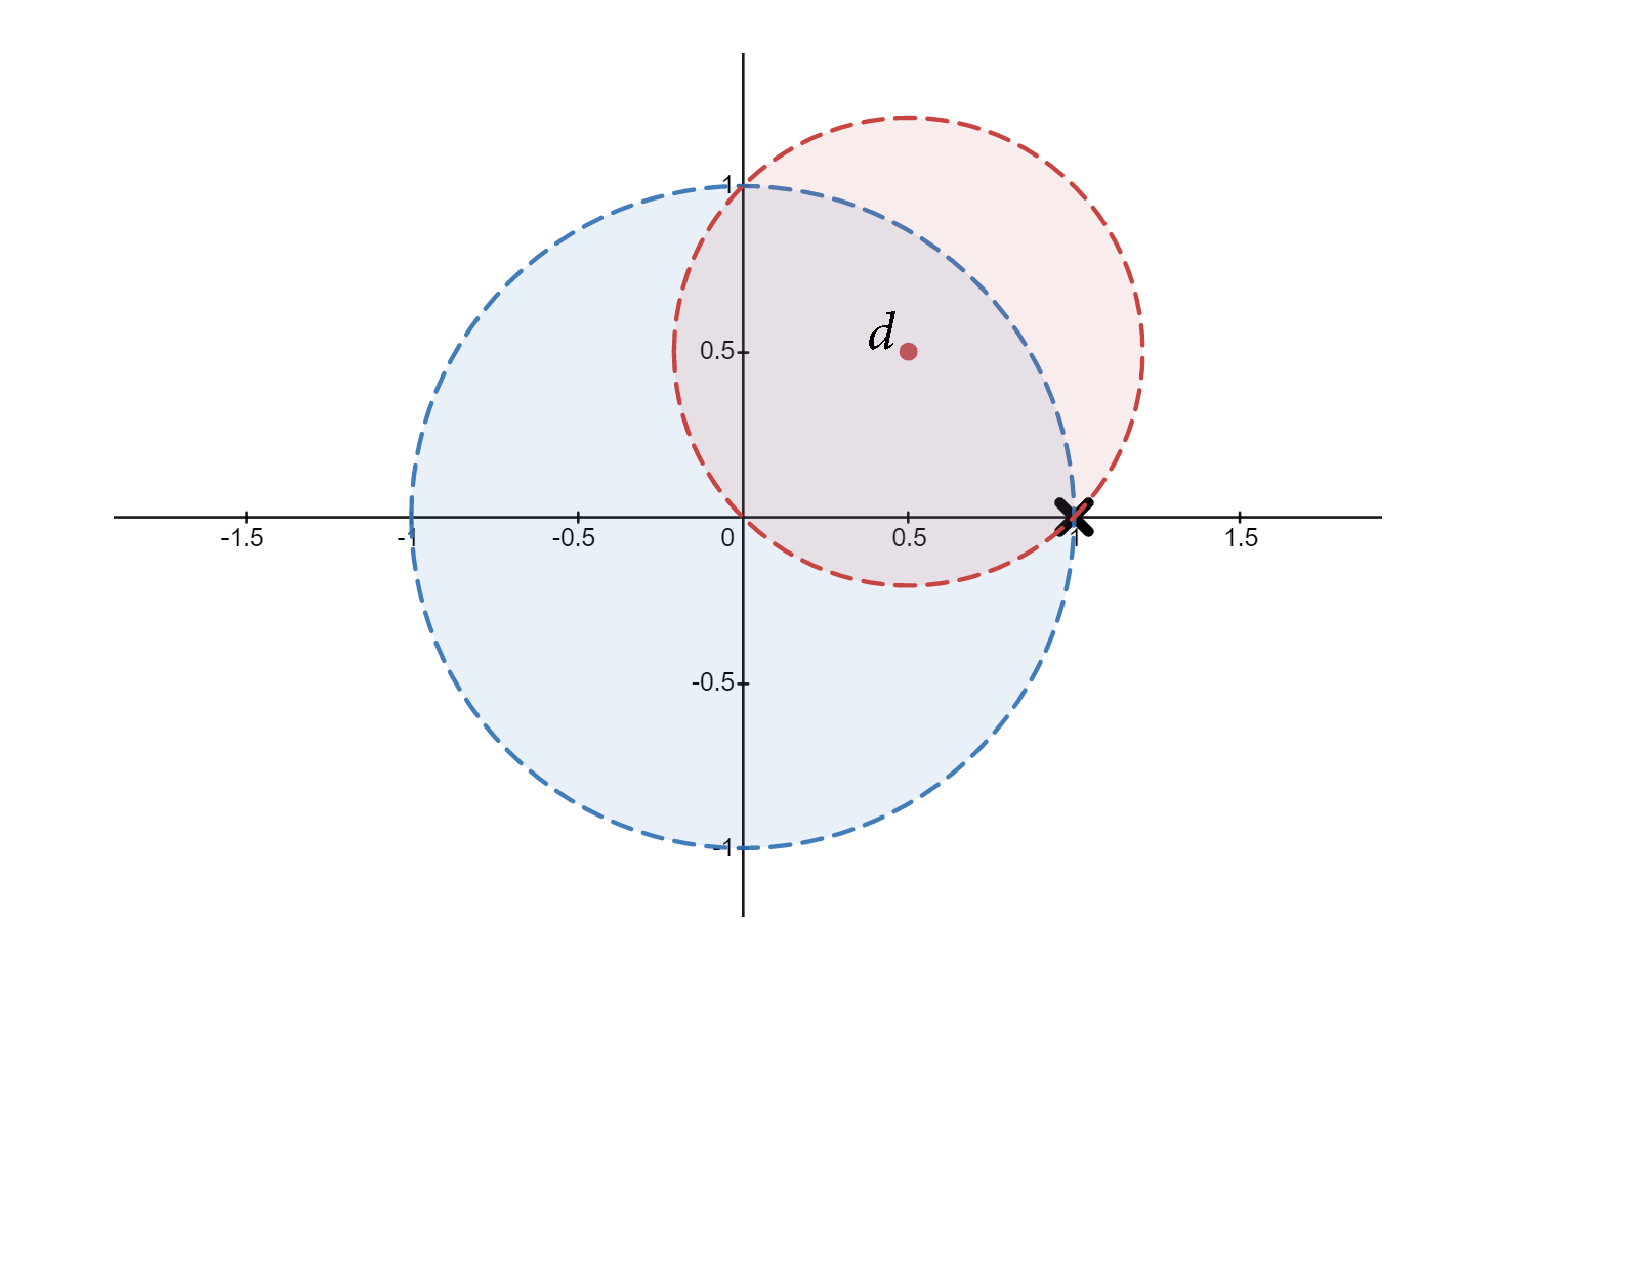
\includegraphics[width=.75\textwidth]{Taylor1.pdf}
    \caption{Graphical representation of the standard method of analytic continuation.}
    \label{Taylor1}
\end{figure}

The resulting series will absolutely converge in any circle centered at $d$ and that circle lies in the circle $|z| = 1$. This series may converge in a larger circle and will provide an analytic continuation of the function as shown in Figure \ref{Taylor1}.

Recall that our goal is to extend the analyticity to the whole complex plane. Thus, we need to perform infinitely many expansions to cover the complex plane. In this case, the standard method of analytic continuation is not practical to use. But, this is still useful if the goal is to extend the analyticity of the function to a specific region.

\subsection{Analytic continuation through the integral representation of digamma function}

We already showed that standard method of analytic continuation is not practical in extending the analyticity of the function to the whole complex plane. In that case, we need to think of a more clever way of extending the function analyticity. Using the zeta function as an inspiration, one may exploit the integral representation of the digamma function. 

One of the integral representation of the digamma function $\psi(z)$ \footnote{Digamma function has a simple pole for all negative integers including zero.} is 
\begin{equation} \label{DGIR}
    \psi(z) = \int_{0}^{1} \frac{1-t^{z-1}}{1-t} \, \mathrm{d}t - \gamma
\end{equation} 
where $\gamma$ is the Euler-Mascheroni constant and exists for $Re(z) > 0$. Directly substituting the above integral representation to the ${}_p\tilde{\psi}_{q}$ written in equation \eqref{psi}, we will have 
\begin{equation}
    \pPq{p}{q}{\Vec{a}}{\Vec{b}}{c}{z} =  \sum_{k=0}^{\infty} \frac{\prod_{l=1}^{p} (a_{l})_k}{ \prod_{l=1}^{q} (b_{l})_k} \left( \int_{0}^{1} \frac{1-t^{k+c-1}}{1-t} \, \mathrm{d}t - \gamma \right) \frac{z^k}{k!}.
\end{equation}
By invoking the convergence of the integral, we can now interchange the integral and summation, resulting to
\begin{align}
\begin{split} 
    \pPq{p}{q}{\Vec{a}}{\Vec{b}}{c}{z} & =\int_{0}^{1} \frac{\sum_{k=0}^{\infty} \frac{\prod_{l=1}^{p} (a_{l})_k}{ \prod_{l=1}^{q} (b_{l})_k} \frac{z^k}{k!} - \sum_{k=0}^{\infty} \frac{\prod_{l=1}^{p} (a_{l})_k}{ \prod_{l=1}^{q} (b_{l})_k} \frac{(tz)^k}{k!} t^{c-1}}{1-t} \, \mathrm{d}t \\& \qquad - \gamma \, \sum_{k=0}^{\infty} \frac{\prod_{l=1}^{p} (a_{l})_k}{ \prod_{l=1}^{q} (b_{l})_k} \frac{z^k}{k!}.
\end{split}
\end{align}
Rewriting the above equation by making the series into hypergeometric function written in equation \eqref{GHF} will result to
\begin{align}
\begin{split} 
    \pPq{p}{q}{\Vec{a}}{\Vec{b}}{c}{z} & =\int_{0}^{1} \frac{\pFq{p}{q}{\Vec{a}}{\Vec{b}}{z} - \pFq{p}{q}{\Vec{a}}{\Vec{b}}{tz}  t^{c-1}}{1-t} \, \mathrm{d}t - \gamma \, \pFq{p}{q}{\Vec{a}}{\Vec{b}}{z}.
\end{split}
\end{align}
The above function is said to exists provided that the hypergeometric function exists and $\mathrm{Re}(c) > 0$. By the principle of analytic continuation, the function is now defined outside the circle, i. e. $|z|>1$. However, the parameter $c$ is still restricted on the right-hand side of the complex plane, i. e. $\mathrm{Re}(c) > 0$. Therefore, we need to think of a way that will extend the analyticity of the function without sacrificing the restriction of the parameters.  

There are two possible ways that will broaden the restriction of parameters without sacrificing its analyticity. First, we will extend the integral representation to the other half-plane before substituting it to the function.  And second, we will perform some manipulation to the function before substituting the integral representation. 

\subsubsection{Integration by parts}

We wish to extend the integral representation of the digamma function to the left side of the complex plane. To do this, we will perform integration by parts on an integral part of equation \eqref{DGIR}. First, we let 
\begin{equation}
    u = \frac{1}{1-t} \Longrightarrow du = \frac{1}{(1-t)^2} \, \mathrm{d}t
\end{equation}
and 
\begin{equation}
\mathrm{d}v = 1-t^{z-1} \, \mathrm{d}t \Longrightarrow v = t - \frac{t^{z}}{z} +C
\end{equation}
where $C$ is a constant. We will choose the constant $C$ such that $t = 1$, doing so, we will get
\begin{equation}
    C = \frac{1}{z} - 1.
\end{equation}
Implementing the integration by parts will result to
\begin{align}
\begin{split} 
    \int_{0}^{1} \frac{1-t^{z-1}}{1-t}\, \mathrm{d}t & = \left.  \frac{t - \frac{t^{z}}{z}+\frac{1}{z} - 1}{1-t} \right|_{0}^{1} - \int_{0}^{1} \frac{t - \frac{t^{z}}{z}+\frac{1}{z} - 1}{(1-t)^2} \, \mathrm{d}t
    \\& = 1 - \frac{1}{z} - \int_{0}^{1} \frac{t - \frac{t^{z}}{z}+\frac{1}{z} - 1}{(1-t)^2} \, \mathrm{d}t.
\end{split}
\end{align}
Obviously, the equality of the above equation will hold for $\mathrm{Re}(z) > 0$. Moreover, looking closely at the right-hand side of the equation, it can be seen that it exists for $\mathrm{Re}(z) > -1$. Using it as a new integral representation of the digamma function, it will give us
\begin{equation} \label{DGIR1}
    \psi(z) = 1 - \frac{1}{z} - \int_{0}^{1} \frac{t - \frac{t^{z}}{z}+\frac{1}{z} - 1}{(1-t)^2} \, \mathrm{d}t - \gamma,
\end{equation} 
which exists for $\mathrm{Re}(z) > -1$. Substituting the above equation to the function $_{p}\tilde{\psi}_{q}$ and using the hypergeometric function in equation \eqref{GHF} to close the series will result to
\begin{align}
\begin{split}
    \pPq{p}{q}{\vec{a}}{\vec{b}}{c}{z} &  = \left(1 -  \gamma\right) \, \pFq{p}{q}{\vec{a}}{\vec{b}}{z} - \frac{1}{c} \, \pFq{p+1}{q+1}{\vec{a}, c}{\vec{b}, c+1}{z} \,
    \\& \quad - \int_{0}^{1} \Bigg[  \pFq{p}{q}{\vec{a}}{\vec{b}}{z} \,  (t-1)  \, 
    \\& \hspace{22mm}  - \frac{1}{c} \, t^{c+1} \pFq{p+1}{q+1}{\vec{a}, c}{\vec{b}, c+1}{tz}   
    \\& \hspace{32mm} + \frac{1}{c} \, \pFq{p+1}{q+1}{\vec{a}, c}{\vec{b}, c+1}{z}     \Bigg] \, \frac{\mathrm{d}t}{(1-t)^2}
\end{split}
\end{align}
for $\mathrm{Re}(c)> -1$. We see that the above equation diverges when $c=0$, which implies that $c=0$ is a pole of the function $_{p}\tilde{\psi}_{q}$ with respect to the parameter $c$. The above series is found to be convergent for all $z$ excluding the singularities and branch cut. From this result, we can conclude that the analyticity of the integral representation of the digamma function together with the parameter $c$ of the function $_{p}\tilde{\psi}_{q}$ can be pushed further to the left side by performing repeated integration by parts. The next question is, can we extend it to the whole left side of the complex plane? To answer this question, we will do some more integration by parts. 

Performing another integration by parts, we will let 
\begin{equation}
    u = \frac{1}{(1-t)^{2}} \Longrightarrow du = \frac{2}{(1-t)^3} \, \mathrm{d}t
\end{equation}
and 
\begin{equation}
\mathrm{d}v =t - \frac{t^{z}}{z}+\frac{1}{z} - 1 \, \mathrm{d}t \Longrightarrow v = \frac{t^2}{2} - \frac{t^{z+1}}{z(z+1)}+\left(\frac{1}{z} - 1\right)t +C
\end{equation}
where $C$ is a constant. Again, we choose the constant $C$ such that $t = 1$, this will result to
\begin{equation}
    C = \frac{1}{z(z+1)}-\frac{1}{z} +\frac{1}{2}.
\end{equation}
Applying the integration by parts technique, will result to
\begin{align}
\begin{split}
    \int_{0}^{1} & \frac{t - \frac{t^{z}}{z}+\frac{1}{z} - 1}{(1-t)^2} \, \mathrm{d}t \\& = \left.  \frac{\frac{t^2}{2} - \frac{t^{z+1}}{z(z+1)}+\left(\frac{1}{z} - 1\right)t + \frac{1}{z(z+1)}-\frac{1}{z} +\frac{1}{2}}{(1-t)^{2}} \right|_{0}^{1}
    \\& \quad - 2\int_{0}^{1} \frac{\frac{t^2}{2} - \frac{t^{z+1}}{z(z+1)}+\left(\frac{1}{z} - 1\right)t+\frac{1}{z(z+1)}-\frac{1}{z} +\frac{1}{2}}{(1-t)^{3}} \, \mathrm{d}t
    \\& = \frac{1}{z(z+1)}-\frac{1}{z} +\frac{1}{2}
    \\& \quad - 2\int_{0}^{1} \frac{\frac{t^2}{2} - \frac{t^{z+1}}{z(z+1)}+\left(\frac{1}{z} - 1\right)t+\frac{1}{z(z+1)}-\frac{1}{z} +\frac{1}{2}}{(1-t)^{3}} \, \mathrm{d}t
\end{split}
\end{align}
Substituting the above equation to equation \eqref{DGIR1}, we will have a new representation of the digamma function expressed as
\begin{align}
\begin{split}
    \psi(z) \,&  = 1-\frac{1}{z} - \left( \frac{1}{z(z+1)}-\frac{1}{z} +\frac{1}{2} \right)
    \\& \quad + 2\int_{0}^{1} \frac{\frac{t^2}{2} - \frac{t^{z+1}}{z(z+1)}+\left(\frac{1}{z} - 1\right)t+\frac{1}{z(z+1)}-\frac{1}{z} +\frac{1}{2}}{(1-t)^{3}} \, \mathrm{d}t
    \\& = \frac{1}{2} - \frac{1}{z(z+1)} - \gamma
    \\& \quad + 2\int_{0}^{1} \frac{\frac{t^2}{2} - \frac{t^{z+1}}{z(z+1)}+\left(\frac{1}{z} - 1\right)t+\frac{1}{z(z+1)}-\frac{1}{z} +\frac{1}{2}}{(1-t)^{3}} \, \mathrm{d}t,
\end{split}
\end{align}
valid for $\mathrm{Re}(c) > -2$. Again, we successfully extend the analyticity of the integral representation of the digamma function. Substituting it to the ${}_p\tilde{\psi}_{q}$ will also extend the analyticity of the function outside the original convergence $|z| < 1$. The new form of the function ${}_p\tilde{\psi}_{q}$ is given by
\begin{align}
\begin{split}
    \pPq{p}{q}{\vec{a}}{\vec{b}}{c}{z} &  = \left(\frac{1}{2} -  \gamma\right) \pFq{p}{q}{\vec{a}}{\vec{b}}{z} - \frac{1}{c+1} \pFq{p+1}{q+1}{\vec{a}, c}{\vec{b}, c+2}{z} 
    \\& \quad + \int_{0}^{1}  \Bigg[ (t^2-2t+1)\, \pFq{p}{q}{\vec{a}}{\vec{b}}{z}  
    \\& \hspace{19mm}  - \frac{2 t^{c+1}}{c+1} \pFq{p+1}{q+1}{\vec{a}, c}{\vec{b}, c+2}{tz}   
    \\& \hspace{19mm}  + \frac{2}{c+1} \pFq{p+1}{q+1}{\vec{a}, c}{\vec{b}, c+2}{z}    
    \\& \hspace{20mm}  - \frac{2 (1+t)}{c} \pFq{p+1}{q+1}{\vec{a}, c+1}{\vec{b}, c+2}{z} \Bigg] \, \frac{\mathrm{d}t}{(1-t)^{3}}
\end{split}
\end{align}
for $\mathrm{Re}(c) > -2$ with a pole singularity at $c = 0$ and $c=1$. However, as we further perform integration by parts to push the analyticity to the left side of the complex plane and fully cover it, the integral becomes more and more complex. One may generalize the integral through a recurrence relation or a generating function. As of the moment, we cannot find a pattern and think of a way to generalize it. Thus, extending the analyticity of the integral representation of the digamma function to the whole complex plane using this technique is difficult as of the moment, but possible. 

\subsubsection{Series decomposition}

In this technique, we will first assume that the parameter $\mathrm{Re}(c) < 0$. Then, we decompose the series into two groups. The first series are the terms where the argument of the real part of the digamma factor in ${}_p\tilde{\psi}_{q}$ is negative, and the second series will have a positive real part argument in the digamma factor. Implementing the decomposition, we will have
\begin{align}
\begin{split}
        \pPq{p}{q}{\Vec{a}}{\Vec{b}}{c}{z} & =  \sum_{k=0}^{\floor*{\mathrm{Re}(-c)}} \frac{\prod_{l=1}^{p} (a_{l})_k}{ \prod_{l=1}^{q} (b_{l})_k} \psi(k+c) \frac{z^k}{k!} \\& \hspace{10mm} + \sum_{k=\floor*{\mathrm{Re}(-c)}+1}^{\infty} \frac{\prod_{l=1}^{p} (a_{l})_k}{ \prod_{l=1}^{q} (b_{l})_k} \psi(k+c) \frac{z^k}{k!}
\end{split}
\end{align}
The first series is defined in the whole complex plane, since it is only a finite series. Also, the parameter $c$ can be any complex number where the digamma function exists. For the second group of series, if $p = q+1$, the function is only defined for $|z| < 1$. Fortunately, we already solve this problem by substituting the integral representation of the digamma function into the infinite series. Also, for the infinite series, we are certain that the digamma function will exists whatever value of $c$ since the argument of the digamma function is always positive. Substituting the integral representation of the digamma function, we will have
\begin{align}
\begin{split}
        \pPq{p}{q}{\Vec{a}}{\Vec{b}}{c}{z} & =  \sum_{k=0}^{\floor*{\mathrm{Re}(-c)}} \frac{\prod_{l=1}^{p} (a_{l})_k}{ \prod_{l=1}^{q} (b_{l})_k} \psi(k+c) \frac{z^k}{k!} \\& \hspace{2mm} + \sum_{k=\floor*{\mathrm{Re}(-c)}+1}^{\infty} \frac{\prod_{l=1}^{p} (a_{l})_k}{ \prod_{l=1}^{q} (b_{l})_k} \left( \int_{0}^{1} \frac{1-t^{k+c-1}}{1-t} \, \mathrm{d}t - \gamma \right) \frac{z^k}{k!}.
\end{split}
\end{align}
Again, invoking the convergence of the integral, we are allowed to interchange the order of the summation and integration
\begin{align}
\begin{split} \label{SD1}
        \pPq{p}{q}{\Vec{a}}{\Vec{b}}{c}{z} & =  \sum_{k=0}^{\floor*{\mathrm{Re}(-c)}} \frac{\prod_{l=1}^{p} (a_{l})_k}{ \prod_{l=1}^{q} (b_{l})_k} \psi(k+c) \frac{z^k}{k!} - \gamma \, \sum_{k=\floor*{\mathrm{Re}(-c)}+1}^{\infty} \frac{\prod_{l=1}^{p} (a_{l})_k}{ \prod_{l=1}^{q} (b_{l})_k} \frac{z^k}{k!}
        \\& \hspace{-15mm} + \int_{0}^{1} \frac{\sum_{k=\floor*{\mathrm{Re}(-c)}+1}^{\infty} \frac{\prod_{l=1}^{p} (a_{l})_k}{ \prod_{l=1}^{q} (b_{l})_k} \frac{z^k}{k!} - \sum_{k=\floor*{\mathrm{Re}(-c)}+1}^{\infty} \frac{\prod_{l=1}^{p} (a_{l})_k}{ \prod_{l=1}^{q} (b_{l})_k} \frac{(tz)^k}{k!}t^{c-1}}{1-t} \, \mathrm{d}t .
\end{split}
\end{align}
Now, we need to close the infinite series. It is done by doing some manipulation to the series to make it a generalized hypergeometric function. Carrying out some manipulation to the summation, we will have
\begin{align}
\begin{split}
    \sum_{k=\floor*{\mathrm{Re}(-c)}+1}^{\infty} & \frac{\prod_{l=1}^{p} (a_{l})_k}{ \prod_{l=1}^{q} (b_{l})_k} \frac{z^k}{k!} \\& \hspace{-10mm} = \sum_{n=0}^{\infty} \frac{\prod_{l=1}^{p} (a_{l})_{n+\floor*{\mathrm{Re}(-c)}+1}}{ \prod_{l=1}^{q} (b_{l})_{n+\floor*{\mathrm{Re}(-c)}+1}} \frac{z^{n+\floor*{\mathrm{Re}(-c)}+1}}{(n+\floor*{\mathrm{Re}(-c)}+1)!}
    \\& \hspace{-10mm} = \frac{\prod_{l=1}^{p} \Gamma(b_l) \Gamma(a_{l}+\floor*{\mathrm{Re}(-c)}+1)}{\prod_{l=1}^{q} \Gamma(a_l) \Gamma(a_{l}+\floor*{\mathrm{Re}(-c)}+1)} \frac{z^{\floor*{\mathrm{Re}(-c)}+1}}{\Gamma(\floor*{\mathrm{Re}(-c)}+2)} \\& \times \sum_{n=0}^{\infty} \frac{\prod_{l=1}^{p} (a_{l}+\floor*{\mathrm{Re}(-c)}+1)_{n} (1)_n}{\prod_{l=1}^{q} (b_{l}+\floor*{\mathrm{Re}(-c)}+1)_{n} (\floor*{\mathrm{Re}(-c)}+2)_{n}} \frac{z^{n}}{n!}
    \\& \hspace{-10mm} = \frac{\prod_{l=1}^{p} (a_{l})_{\floor*{\mathrm{Re}(-c)}+1}}{\prod_{l=1}^{q} (b_{l})_{\floor*{\mathrm{Re}(-c)}+1}} \frac{z^{\floor*{\mathrm{Re}(-c)}+1}}{\Gamma(\floor*{\mathrm{Re}(-c)}+2)} \\& \times \pFq{p+1}{q+1}{\Vec{a}+\floor*{\mathrm{Re}(-c)}+1, 1}{\Vec{b}+\floor*{\mathrm{Re}(-c)}+1, \floor*{\mathrm{Re}(-c)}+2}{z}
\end{split}
\end{align}
Substituting the closed form of the infinite series, the hypergeometric function in equation \eqref{GHF} to equation \eqref{SD1}
\begin{align}
\begin{split} 
        & \pPq{p}{q}{\Vec{a}}{\Vec{b}}{c}{z} =  \sum_{k=0}^{\floor*{\mathrm{Re}(-c)}} \frac{\prod_{l=1}^{p} (a_{l})_k}{ \prod_{l=1}^{q} (b_{l})_k} \psi(k+c) \frac{z^k}{k!} 
        \\& \hspace{10mm} + \frac{\prod_{l=1}^{p} (a_{l})_{\floor*{\mathrm{Re}(-c)}+1}}{\prod_{l=1}^{q} (b_{l})_{\floor*{\mathrm{Re}(-c)}+1}} \frac{z^{\floor*{\mathrm{Re}(-c)}+1}}{\Gamma(\floor*{\mathrm{Re}(-c)}+2)} \\&  \hspace{15mm} \times \Bigg[ \int_{0}^{1} \Bigg( \frac{\pFq{p+1}{q+1}{\Vec{a}+\floor*{\mathrm{Re}(-c)}+1, 1}{\Vec{b}+\floor*{\mathrm{Re}(-c)}+1, \floor*{\mathrm{Re}(-c)}+2}{z}}{1-t} 
        \\& \hspace{20mm} - \frac{\pFq{p+1}{q+1}{\Vec{a}+\floor*{\mathrm{Re}(-c)}+1, 1}{\Vec{b}+\floor*{\mathrm{Re}(-c)}+1, \floor*{\mathrm{Re}(-c)}+2}{tz}t^{\floor*{\mathrm{Re}(-c)}+c}}{1-t} \Bigg) \, \mathrm{d}t 
        \\& \hspace{20mm} - \gamma \, \pFq{p+1}{q+1}{\Vec{a}+\floor*{\mathrm{Re}(-c)}+1, 1}{\Vec{b}+\floor*{\mathrm{Re}(-c)}+1, \floor*{\mathrm{Re}(-c)}+2}{z} \Bigg].
\end{split}
\end{align}
Notice that the function is already valid for $|z| > 1$ and the integral is also observed to exists for $\mathrm{Re(c) > 0}$. Therefore, the above expression exists for $\mathrm{Re(c) > 0}$ provided that we interpret the empty sum as zero. This lifting of the initial assumption $\mathrm{Re(c) < 0}$ can be explained by the concept of analytic continuation. 

Finally, we successfully extend the analyticity of the function ${}_p\tilde{\psi}_{q}$ for the whole complex plane and expanding the restriction for the parameter $c$.

\section{Relation of the function $_{p}\tilde{\psi}_{q}$ to Kampé de Fériet function}

To derive a relation between the $_{p}\tilde{\psi}_{q}$ function and Kampé de Fériet function, we will first define an auxiliary function 
\begin{equation}
    G(\mu, \sigma) = \frac{\Gamma(\mu)}{\Gamma(\sigma)} \pFq{p+1}{q+1}{\Vec{a}, \mu}{\Vec{b}, \sigma}{z}
\end{equation}
where all the parameters are taken to be independent of each other. The auxiliary function has a series representation of
\begin{equation}
    G(\mu,\sigma)= \sum_{k=0}^{\infty} \frac{\Gamma(k+\mu)}{\Gamma(k+\sigma)} \frac{\prod_{l=1}^{p} (a_l)_k}{\prod_{l=1}^{q}(b_l)_k} \frac{z^k}{k!} .
\end{equation}
Performing a partial differentiation with respect to $\mu$ and evaluating $\sigma$ at $\mu$, we will have
\begin{equation} \label{4.39}
\left.\frac{\partial G(\mu,\sigma)}{\partial \mu}\right|_{\sigma=\mu} = \sum_{k=0}^{\infty} \frac{\Gamma'(k+\mu)}{\Gamma(k+\mu)} \frac{\prod_{l=1}^{p} (a_l)_k}{\prod_{l=1}^{q}(b_l)_k}\frac{z^k}{k!}. 
\end{equation}
The known relation of the digamma function to a gamma function is just
\begin{equation}
    \psi(z) = \frac{\Gamma'(z)}{\Gamma(z)}.
\end{equation}
Using the fact above, we can rewrite equation \eqref{4.39} as
\begin{equation}
\left.\frac{\partial G(\mu,\sigma)}{\partial \mu}\right|_{\sigma=\mu} = \sum_{k=0}^{\infty}  \frac{\prod_{l=1}^{p} (a_l)_k}{\prod_{l=1}^{q}(b_l)_k} \psi(k+\mu) \frac{z^k}{k!}. 
\end{equation}
We can see that the right-hand side of the equation is just the function ${}_p\tilde{\psi}_{q}$ written in equation \eqref{psi}. Also, performing a similar operation to the equation will results in the evaluation of infinite series in terms of derivative of the hypergeometric function. The following result can be readily established as 
\begin{equation}
\left.\frac{\partial G(\mu,\sigma)}{\partial \mu}\right|_{\sigma=\mu} = \psi(\mu)\; \pFq{p}{q}{\vec{a}}{\vec{b}}{z} + \left.\frac{\partial}{\partial\mu}  \pFq{p+1}{q+1}{\mu,\vec{a}}{\sigma,\vec{b}}{z} \right|_{\sigma=\mu} .
\end{equation}
Equating the two equations, we will have
\begin{equation}
    \pPq{p}{q}{\vec{a}}{\vec{b}}{\mu}{z} =  \psi(\mu)\; \pFq{p}{q}{\vec{a}}{\vec{b}}{z} + \left.\frac{\partial}{\partial\mu}  \pFq{p+1}{q+1}{\mu,\vec{a}}{\sigma,\vec{b}}{z} \right|_{\sigma=\mu}.
\end{equation}
Now, we evaluate the partial derivative of the above equation. The evaluation of the differentiation of the hypergeometric function was already done in \cite{ancarani2010derivatives}. The partial derivative will be evaluated the known result
\begin{equation} \label{4.44}
\frac{\mathrm{d} (\mu)_k}{\mathrm{d}\mu} = (\mu)_k \left[\psi(k+\mu)-\psi(\mu)\right].
\end{equation}
Using the transformation of digamma function \cite{digamma}
\begin{equation}
\psi(n+z)= \psi(z)+\sum_{s=0}^{n-1}\frac{1}{s+z},\;\; n=1, \, 2, \dots ,
\end{equation}
and
\begin{align}
\begin{split}
    \frac{1}{s+z} =\frac{1}{z}\frac{(z)_s}{(z+1)_s},
\end{split}
\end{align}
equation \eqref{4.44} becomes
\begin{equation}
\frac{\mathrm{d}(\mu)_k}{\mathrm{d}\mu} =\frac{(\mu)_k}{\mu}\sum_{s=0}^{k-1}\frac{(\mu)_s}{(\mu+1)_s}.
\end{equation}
Take note that the sum on the right hand is zero when it's an empty sum. Using the above equation, the term by term differentiation of the infinite series representation of the hypergeometric function will lead to
\begin{equation}\label{partial2}
\left.\frac{\partial}{\partial\mu}  \pFq{p+1}{q+1}{\mu,\vec{a}}{\sigma,\vec{b}}{z}\right|_{\sigma=\mu} = \sum_{k=0}^{\infty}\sum_{s=0}^k \frac{ (\mu)_s (\vec{a})_{k+1}}{(\mu+1)_s  (\vec{b})_{k+1}} \frac{z^{k+1}}{(k+1)!} .
\end{equation}
Now, we will rearrange the double sum to assume the form of the known Gaussian hypergeometric series of two variables. In that case, we will use the double sum rearrangement formula
\begin{equation}
\sum_{k=0}^{\infty}\sum_{s=0}^k B(s,k) = \sum_{k=0}^{\infty}\sum_{s=0}^{\infty} B(s,k+s).
\end{equation}
Invoking the rearrangement formula, we will have
\begin{align}
\begin{split} \label{HtKdF}
 &\left.\frac{\partial}{\partial\mu} \pFq{p+1}{q+1}{\mu,\vec{a}}{\sigma,\vec{b}}{z}\right|_{\sigma=\mu} 
 \\& \hspace{30mm} = \frac{z}{\mu} \frac{ (\vec{a})_1}{(\vec{b})_1} \sum_{k,s=0}^{\infty} \frac{\prod_{l=1}^p  (a_l+1)_{k+s} (\mu)_s (1)_k (1)_s}{(2)_{k+s} \prod_{l=1}^q (b_j+1)_{k+s} (\mu+1)_s}\, \frac{z^k}{k!} \frac{z^s}{s!} .   
\end{split}
\end{align}
The above double series assume the series representation of the Kampé de Fériet function expressed in equation \eqref{kampein}. With the proper identification of the parameters, we will obtain
\begin{align}
\begin{split}
&\left.\frac{\partial}{\partial\mu}  \pFq{p+1}{q+1}{\mu,\vec{a}}{\sigma,\vec{b}}{z}\right|_{\sigma=\mu} \\& \hspace{30mm} = \frac{z}{ \mu} \frac{ (\vec{a})_1}{(\vec{b})_1} \; F^{p:\;1;\;2}_{q+1:- ;\;1}\left[\begin{array}{lll}
\vec{a}+1&: 1 &; \mu,1  \\
2, \vec{b}+1&:- &; \mu+1 
\end{array};\; z,z\right] .
\end{split}
\end{align}
Collecting all our results, we obtain the relation of the function ${}_{p}\tilde{\psi}_{q}$ to 
\begin{align}
\begin{split} \label{DxKv0}
    \pPq{p}{q}{\Vec{a}}{\Vec{b}}{\mu}{z} & = \psi(\mu) \pFq{p}{q}{\Vec{a}}{\Vec{b}}{z} \\& + \frac{z}{\mu} \frac{(\Vec{a})_1}{(\Vec{b})_1} F^{p:\;1;\;2}_{q+1:\;-;\;1}\left[\begin{array}{ccc}
     \Vec{a}+1:& 1; & \mu, 1  \\
     2, \Vec{b}+1:& ; & \mu+1 
    \end{array};\;  z,z\right] .
\end{split}
\end{align}
The above results is itself a reduction formula of the Kampé de Fériet function and it will be written as a theorem.

\begin{theorem}
The family of reduction formula of the Kampé de Fériet function can be expressed in terms of the ${}_{p}\tilde{\psi}_{q}$ function and generalized hypergeometric function ${}_pF_{q}$
\begin{align}
\begin{split} \label{DxK}
     F^{p:\;1;\;2}_{q+1:\;-;\;1}\left[\begin{array}{ccc}
     \Vec{a}+1:& 1; & \mu, 1  \\
     2, \Vec{b}+1:& ; & \mu+1 
    \end{array};\;  z,z\right] &\\&  \hspace{-35mm} = \frac{\mu}{z} \frac{(\vec{b})_1}{(\vec{a})_2} \Bigg[ \pPq{p}{q}{\Vec{a}}{\Vec{b}}{\mu}{z}  - \psi(\mu) \pFq{p}{q}{\Vec{a}}{\Vec{b}}{z}  \Bigg].
\end{split}
\end{align}
\end{theorem}

We will exploit the above theorem in the next chapter to obtain a reduction formula of the Kampe de Feiret function.

\chapter{Reduction Formula of Kampé de Fériet function}


\label{ch_5}
\hspace{\parindent}

From chapter \ref{ch_3}, we see how the summation involving digamma function naturally arises in the calculation of the finite-part integral, specifically in the case of pole singularity. While in chapter \ref{ch_4}, we obtain the relation of this summation to the reduction formula of Kampé de Fériet function. In this chapter, we will exploit the result of the exact evaluation of the Stieltjes transform and use the established relation from the previous chapter to tabulate reduction formulas of the Kampé de Fériet function. 

All of the theorems and corollaries presented in this chapter were numerically verified. Numerical verification means that both side of the equation will be evaluated numerically for a random set of parameters and compare their numerical values. The equality holds if both right hand sides of the equation agree to the same numerical value. The code in Mathematica notebook used in the numerical verification can be found in the Appendix \ref{mathematica}. The code with $10$ digits of precision were executed on the following specifications: Intel i5-9300H processor CPU @ 2.40 GHz and 16GB RAM. The code were all written in Wolfram Mathematica v12.1.

\section{Reduction formula from Generalized Stieltjes transform of $f(x) = e^{-bx}$}

According to \cite{erdelyi1954tables}, the generalized Stietljes transform of $f(x) = e^{-bx}$ for integral order is known to be 
\begin{equation} \label{5.1}
    \int_0^{\infty} \frac{e^{-bx}}{(\omega + x)^{n}} \, \mathrm{d}x = b^{n-1}e^{b\omega} \, \Gamma(1-n,\, b\omega),
\end{equation}
for $\mathrm{Re}(b)>0$ and $|\mathrm{arg}(\omega)|>\pi$. The $\Gamma(s,x)$ factor refers to the incomplete gamma function, which is expressed as
\begin{equation}
    \Gamma(s,x) = \int_{x}^{\infty} t^{s-1} \, e^{-t} \, \mathrm{d}t.
\end{equation} 
The integral will be evaluated using the method of finite-part integration. Obviously, when we expand the kernel, we will have a pole singularity. Therefore, we will use Theorem \ref{T3.3} to evaluate the integral. Invoking the theorem, we will have the expression
\begin{equation} \label{5.2}
    \int_0^{\infty} \frac{e^{-bx}}{(\omega + x)^{n}} \mathrm{d}t = \sum_{k=0}^{\infty} \binom{-n}{k} \omega^{k} \bbint{0}{\infty} \frac{e^{-bx}}{x^{k+n}} \, \mathrm{d}x + \Delta_{\mathrm{sc}}^{(n)}(\omega).
\end{equation}
where 
\begin{equation}
\begin{split} \label{sc4.1}
    \Delta_{\mathrm{sc}}^{(n)}(\omega) & =  -\frac{\ln{\omega}}{\Gamma(n)} \left. \frac{\mathrm{d}^{n-1}}{\mathrm{d}z^{n-1}} \,  e^{-bz} \right|_{z=-\omega} + \sum_{k=0}^{n-2} \frac{\omega^{k-n+1}}{k!(n-1-k)} \left. \frac{\mathrm{d}^{k}}{\mathrm{d}z^{k}} \,  e^{-bz} \right|_{z=-\omega} 
    \\& = -\frac{\ln{\omega}}{\Gamma(n)} (-b)^{n-1} e^{b\omega} + \sum_{k=0}^{n-2} \frac{\omega^{k-n+1}}{k!(n-1-k)} (-b)^{k} e^{b\omega}
\end{split}
\end{equation}
Using the tabulated list of evaluated finite-part integral in \cite{ticathetit}, the finite-part integral from the above equation is calculated to be
\begin{equation}
    \bbint{0}{\infty} \frac{e^{-bx}}{x^{k+n}} \, \mathrm{d}x = \frac{(-1)^{k+n} b^{k+n-1}}{\Gamma(k+n)} (\ln{b} - \psi(k+n))
\end{equation}
We will substitute the evaluated finite-part integral and equation \eqref{sc4.1} to equation \eqref{5.2}. Then, we will rewrite the combination in terms of gamma function and express the summation of digamma function as ${}_p\tilde{\psi}_{q}$ using equation \eqref{psi}. The desired integral will assume the form
\begin{equation}
\begin{split} \label{5.4}
    \int_0^{\infty} \frac{e^{-bx}}{(\omega + x)^{n}} = & \frac{(-1)^n \, b^{n-1}}{\Gamma(n)} \Bigg[ \sum_{k=0}^{\infty} \frac{(\omega b)^{k}}{k!} \ln{b} - \pPq{0}{0}{}{}{n}{b\omega} \Bigg]
    \\& -\frac{\ln{\omega}}{\Gamma(n)} (-b)^{n-1} e^{b\omega} + \sum_{k=0}^{n-2} \frac{\omega^{k-n+1}}{k!(n-1-k)} (-b)^{k} e^{b\omega}.
\end{split}
\end{equation}
Now, we see the infinite series with logarithmic factor can be simplified into exponential function. Combining the similar terms, we will have
\begin{equation}
\begin{split} \label{5.5}
    \int_0^{\infty} \frac{e^{-bx}}{(\omega + x)^{n}} = & -\frac{(-1)^{n} \, b^{n-1}}{\Gamma(n)} \pPq{0}{0}{}{}{n}{b\omega} - \frac{(-b)^{n-1} e^{b \omega}}{\Gamma(n)} \ln{b\omega}
    \\& - b^{n-1}\sum_{k=0}^{n-2} (-1)^{k} \frac{(b\omega)^{k-n+1}}{k!(n-1-k)} e^{b\omega}.
\end{split}
\end{equation}
Next, we will use the relation of the function ${}_p\tilde{\psi}_{q}$ to the Kampé de Fériet function express in \eqref{DxKv0} to arrive to this relation
\begin{equation} \label{5.6}
    \pPq{0}{0}{}{}{n}{b\omega} = \psi(n) e^{b\omega} + \frac{b\omega}{n} F^{-:\;1;\;2}_{1:\;-;\;1}\left[\begin{array}{ccc}
     -:& 1; & 1, n  \\
     2:& -; & n+1 
    \end{array};\;  b\omega,b\omega\right].
\end{equation}
Putting back equation \eqref{5.6} to equation \eqref{5.5} and substituting \eqref{5.1} to the left hand side of \eqref{5.5}, will yield to
\begin{equation}
\begin{split}
    b^{n-1} e^{b\omega} \,& \Gamma(1-n,\, b\omega) \\& = -\frac{(-1)^n \, b^{n-1}}{\Gamma(n)} \left(  \psi(n) e^{b\omega} + \frac{b\omega}{n} F^{-:\;1;\;2}_{1:\;-;\;1}\left[\begin{array}{ccc}
     -:& 1; & 1, n  \\
     2:& -; & n+1 
    \end{array};\;  b\omega,b\omega\right] \right) \\& - \frac{(-b)^{n-1}}{\Gamma(n)} e^{b \omega} \ln{b\omega} - b^{n-1}\sum_{k=0}^{n-2} (-1)^{k} \frac{(b\omega)^{k-n+1}}{k!(n-1-k)} e^{b\omega}.
\end{split}
\end{equation}
Simplifying it further by combining similar terms and letting $z = b\omega$ will result to
\begin{equation}
\begin{split}
     e^{z} \,& \Gamma(1-n,\, z) = -\frac{(-1)^n}{\Gamma(n)} \frac{z}{n} F^{-:\;1;\;2}_{1:\;-;\;1}\left[\begin{array}{ccc}
     -:& 1; & 1, n  \\
     2:& -; & n+1 
    \end{array};\;  z,z\right] \\& - \frac{(-1)^{n-1}}{\Gamma(n)} e^{b \omega} (\ln{z} - \psi(n)) - \sum_{k=0}^{n-2} (-1)^{k} \frac{(z)^{k-n+1}}{k!(n-1-k)} e^{z}.
\end{split}
\end{equation}
By the concept of analytic continuation, the value of $z$ extends to the complex plane. Also, the reduction formula of the Kampé de Fériet function is obtained by isolating the function. 

\begin{theorem}
For complex number $z$ and positive integer $n$ the reduction formula of the Kampé de Fériet function is equal to
\begin{equation}
\begin{split}
      F^{-:\;1;\;2}_{1:\;-;\;1}\left[\begin{array}{ccc}
     -:& 1; & 1, n  \\
     2:& -; & n+1 
    \end{array};\;  z,z\right] & \\&\hspace{-20mm} = \frac{n \, e^{z}}{z} \Bigg[\mathrm{Log}(z) -\psi(n) - \frac{\Gamma(n)}{(-1)^{n}} \Gamma(1-n,\,z) \\&\hspace{2mm} + \frac{\Gamma(n)}{(-z)^{n-1}} \sum_{k=0}^{n-2} \frac{(-z)^{k}}{k!(n-1-k)}
    \Bigg],
\end{split}
\end{equation}
where all the functions is taken as their principal value.
\end{theorem}

 \begin{figure}[t]
 	\centering
 	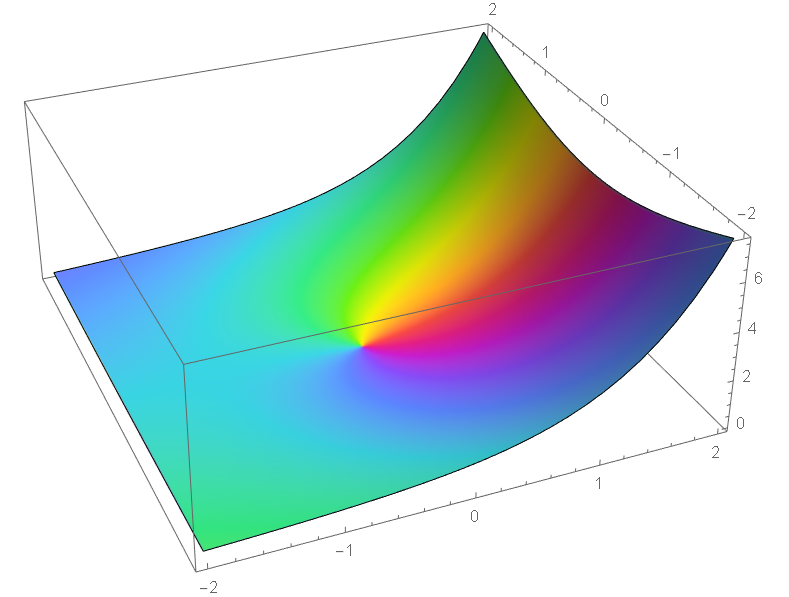
\includegraphics[width=0.75\textwidth]{4.1LHS.png}
 	 	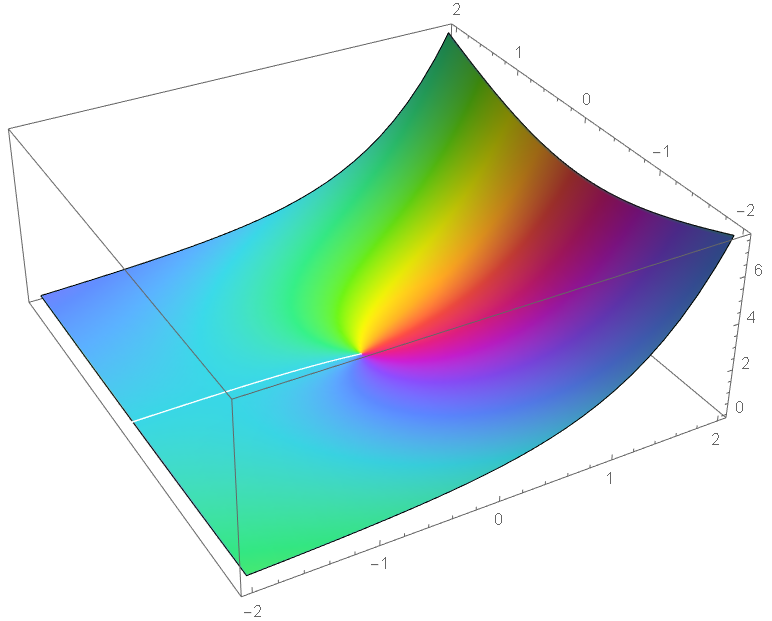
\includegraphics[width=0.75\textwidth]{4.1RHS.png}
 	\caption{The complex plot of the theorem \eqref{4.1} for $n = 2$. (Top) The left-hand side of equality. (Bottom) The right-hand side of the equality. For both plots, the $x$-axis refers to the real-part, the $y$-axis define as the imaginary part, the $z$-axis is the absolute value of the expression $\mathrm{Abs}(f)$, and the color refers to the argument of the expression $\mathrm{Arg}(f)$. Both figures generated using Wolfram Mathematica v12.1.}
 	\label{F4.1}
 \end{figure}

\noindent For accuracy check, we plot the equation of the theorem for $n=2$ into the complex plane. The plot for both sides of the equation is in Figure \ref{F4.1}. We can see that the two figures are almost identical, and we observe a visible branch cut in the figure of the right-hand side. Take note that Mathematica numerically evaluate each functions and terms individually. Thus, the appearance of branch cut is due to the of numerical artifacts of the logarithmic function $\log (z)$ and the incomplete gamma function \cite{incgamma2}
\begin{equation}
\begin{split} \label{IG}
    \Gamma(-n,\,z) = & \frac{(-1)^{n-1}}{n!} \left[ \mathrm{Ei}(-z) - \frac{1}{2} \left( \log(-z) - \log \left( \frac{-1}{z} \right) \right) + \log(z) \right] \\& \hspace{5mm} - e^{-z} \sum_{k=1}^{n} \frac{z^{k-n-1}}{(-n)_k},
\end{split}
\end{equation}
found in the right-hand side of the equation. We can see that both terms have an opposite sign and a branch cut on the same interval. This will make the branch cut to cancel each other and prove the consistency of the complex plot. Finally, the complex plot confirms the accuracy of the established theorem.

Another accuracy check is the simplification of the obtained reduction formula into some known special values. The reduction formula of the Kampé de Fériet Function in Theorem \ref{4.1} is found to be related to the hypergeometric function ${}_2F_2$  \cite[p. 3013, Eq. 3.2a]{miller2006summations}
\begin{equation}
\begin{split}
     F^{-:\;1;\;2}_{1:\;-;\;1}\left[\begin{array}{ccc}
     -:& 1; & 1, n  \\
     2:& -; & n+1 
    \end{array};\;  z,z\right]  = e^z \pFq{2}{2}{1,1}{2,n+1}{-z}.
\end{split}
\end{equation}
Thus, we can extract from the Theorem \ref{4.1} the expression:
\begin{corollary}
For complex number $z$ and positive integer $n$ the hypergeometric function ${}_2F_2$ holds the equality
\begin{equation}
\begin{split}
    \pFq{2}{2}{1,1}{2,n+1}{-z} = & \frac{n}{z} \Bigg[\mathrm{Log}(z) -\psi(n) - \frac{\Gamma(n)}{(-1)^{n}} \Gamma(1-n,\,z) \\& \hspace{20mm} + \frac{\Gamma(n)}{(-z)^{n-1}} \sum_{k=0}^{n-2} \frac{(-z)^{k}}{k!(n-1-k)} \Bigg].
\end{split}
\end{equation}
where all the functions is taken as their principal value.
\end{corollary}

The above expression was tabulated in Wolfram Function site \cite{wolfram2F2} for the cases from $n=1$ up to $n=5$. To confirm the accuracy of the Theorem \ref{4.1}, we need to reproduce the tabulated results. First, let us try for $n=1$, the above equation will give us
\begin{equation}
\begin{split} \label{n1}
    \pFq{2}{2}{1,1}{2,2}{-z} = & \frac{1}{z} \Bigg[\log(z) -\psi(1) + \Gamma(0,\,z) \Bigg].
\end{split}
\end{equation}
Using the fact that $\psi(1) = -\gamma$ where $\gamma$ is the Euler-Mascheroni constant, and the incomplete gamma function $\Gamma(0,\,z)$ \cite{incgamma} is found to be 
\begin{equation}
    \Gamma(0,\,z) = -\mathrm{Ei}(-z) + \frac{1}{2} \left( \log(-z) - \log \left( -\frac{1}{z} \right) \right) - \log(z),
\end{equation}
where $\mathrm{Ei}$ is an exponential integral. Equation \eqref{n1} will reduce to 
\begin{equation}
    \pFq{2}{2}{1,1}{2,2}{-z} =  \frac{1}{2z} \Bigg[2\gamma - 2\mathrm{Ei}(-z) +  \log(-z) - \log \left( -\frac{1}{z} \right) \Bigg].
\end{equation}
The above equation reproduce the hypergeometric function ${}_2F_2(1,1;2,2;z)$ listed in \cite{2f21}. The rest of the tabulated result can be reproduce using the recurrence relation of the digamma function \cite[Eq.~5.5.2]{NIST:DLMF} express as
\begin{equation} 
    \psi(n+1) = \psi(n) + \frac{1}{n},
\end{equation}
and the incomplete gamma function express in equation \eqref{IG}.


\section{Reduction formula from integral representation of Gauss hypergeometric function ${}_2F_1$}

In \cite{saxena1959study}, we can find a more general form of the Stietljes transform evaluated in Chapter \ref{ch_3}. The Stieltjes transform is known to be proportional to the Gauss hypergeometric function,
\begin{equation}
\int_0^{\infty} \frac{x^{\nu-1} (a+x)^{-\mu}}{(b+x)^{\rho}} \, \mathrm{d}x = \frac{\Gamma(\nu) \Gamma(\mu-\nu+\rho)}{\Gamma(\mu+\rho)} \frac{b^{\nu-\rho}}{a^{\mu}}\, \pFq{2}{1}{\mu,\nu}{\mu+\rho}{1-\frac{b}{a}},
\label{STGHF2}
\end{equation}
for $|\mathrm{Arg} \, b|<\pi$, $\mathrm{Re} (\rho+\mu-\nu)>0$. From Chapter \ref{ch_3}, we see how the summation of the digamma function arises in finite-part integral calculation specifically for the pole singularity case. Therefore, we can expect that the summation will appear for the cases where $\nu$ and $\rho$ are integers and $\nu$ and $\rho$ are non-integers with an integer difference. We will exploit the proportionality above to obtain a reduction formula of the Kampé de Fériet function.  

\subsection{Case 1: $\nu$, $\rho \in \mathbb{Z}^{+}$}

In this case, we will consider $\mu$ as any positive real number since we will choose the singularity of $f(z)$ to be located far away or $|a| > |b|$. Thus, the nature of singularity of $(a+z)^{-\mu}$ will not matter. Additionally, we will let $n = \rho$ and $m = \nu$ to be easily identified as a positive integer, $n, m \in \mathbb{Z}^{+}$. Under these conditions, the divergence will induce by the pole singularity. Therefore, we will use Theorem \ref{T3.1} to construct the finite-part integral. Implementing Theorem \ref{T3.3}, the Stieltjes transform of $(a+x)^{-\mu}$ is evaluated to be 
\begin{equation}
\begin{split}
\int_0^{\infty} \frac{x^{m-1} (a+x)^{-\mu}}{(b+x)^{n}} \, \mathrm{d}x =& \sum_{k=0}^{\infty} \, {- n \choose k} \, b^{k} \,\bbint{0}{\infty} \frac{(a+x)^{-\mu}}{x^{k+n-m+1}} \,\mathrm{d}x \\
& - \mathrm{Res} \left[ \frac{z^{m-1} \, (a+z)^{-\mu}}{(b+z)^{n}}\, \log(-z)\right]_{z=-b}.
\end{split} \label{mlessn}
\end{equation}
However, the above equality will only hold when $m < n$. Notice that the terms of the summation when $m \geq n$, the finite-part integral of the terms $0 \leq k \leq m-n-1$ is just a convergent integral. Recall the remarks in \cite{doi:10.1063/5.0038274}, the finite-part integral of a convergent integral is the value of convergent integral itself. Therefore, for $m \geq n$, the Stieltjes transform is
\begin{equation}
\begin{split} \label{mgeqn}
\int_0^{\infty} \frac{x^{m-1} (a+x)^{-\mu}}{(b+x)^{n}} \, \mathrm{d}x =& \sum_{k=0}^{m-n-1} \, {- n \choose k} \, b^{k}   \int_0^{\infty} \frac{(a+x)^{-\mu}}{x^{k+n-m+1}} \,\mathrm{d}x \\& + \sum_{k=m-n}^{\infty} \, {- n \choose k} \, b^{k} \,\bbint{0}{\infty} \frac{(a+x)^{-\mu}}{x^{k+n-m+1}} \,\mathrm{d}x \\
& - \mathrm{Res} \left[ \frac{z^{m-1} \, (a+z)^{-\mu}}{(b+z)^{n}}\, \log(-z)\right]_{z=-b}.
\end{split}
\end{equation}

The first term of the right-hand side of the equation is a convergent integral. It can evaluate easily using the integral representation of the Beta function given by equation
\begin{equation}
\int_0^{\infty} \frac{x^{d-1}}{(1+c x)^{\sigma}}\,\mathrm{d}x = c^{-d} B(d,\sigma-d),\;\; |\mathrm{arg}\,c|<\pi , \;\; \mathrm{Re}\, \sigma > \mathrm{Re}\, d>0,
\end{equation}
where $B(a,b)=\Gamma(a)\Gamma(b)/\Gamma(a+b)$ is the beta function. Applying it to our integral and doing some algebraic manipulation, we obtain the result
\begin{equation}
\int_0^{\infty} \frac{(a+x)^{-\mu}}{ x^{k+n-m+1}} \,\mathrm{d}x
= \frac{\Gamma (-k+m -n )  \Gamma (k+\mu -m +n )}{a^{k+\mu -m +n } \Gamma (\mu
   )}.
\label{BetaInt}
\end{equation}
Next, for the evaluation of the finite-part integral. we will consider the proposition below. 

\begin{proposition} \label{4.1}
Let $n, m$ be a natural number, and $a$, $\mu$ a positive real number. Then
\begin{equation}
\begin{split} \label{fp}
\bbint{0}{\infty} \frac{(a+x)^{-\mu}}{x^{k+n-m+1}}\,\mathrm{d}x = \, &\frac{1}{a^{k+n-m+\mu}} {-\mu \choose k+n-m} \\
& \hspace{-15mm} \times  \left(\log(a) + \psi(k+n-m+1) - \psi(k+n-m+\mu)\right)
\end{split}
\end{equation}
where $\psi(x)$ is a digamma function.
\end{proposition}

\begin{proof}
To prove the above equality, we consider the usual integral with a limits from $\epsilon$ to $c$
\begin{equation}
    \int_{\epsilon}^{c} \frac{(a+x)^{-\mu}}{x^{k+n-m+1}}\,\mathrm{d}x.
\end{equation}
Also, we will expand the binomial $(a+x)^{-\mu}$ at the origin. The expansion is given by
\begin{equation}
    (a+x)^{-\mu} = \sum_{l=0}^{\infty} = {-\mu \choose l} \frac{x^{l}}{a^{l+\mu}},
    \label{TE}
\end{equation} 
which is uniformly convergent for $|x| < a$. The term-wise integration is valid since the function $(a+x)^{-\mu}$ is integrable along the limits of integral $[0,c]$ and well-defined within the radius of convergence of the series. The integral will result to
\begin{equation}
\int_{\epsilon}^{c} \frac{(a+x)^{-\mu}}{x^{k+\rho-m+1}} \,\mathrm{d}x =  \sum_{l=0}^{\infty} {-\mu \choose l}  \frac{1}{a^{l+\mu}} \, \int_{\epsilon}^{c} x^{l-k-n+m-1} \,\mathrm{d}x .
\label{FPIcase1}
\end{equation}
Now, we will decompose the summation into three parts based on the results of the integral. First, the interval $0 \leq l \leq k+\rho-m-1 $ where the integral will result in a negative exponent when evaluated. The integral on term $l = k +\rho -m$ will result in a logarithm. The last interval $k +\rho - m +1 \leq l \leq \infty$ will result to the positive exponent of the integral. Performing the integral and evaluating at the limit of integration will give us
\begin{align}
\begin{split}
\int_{\epsilon}^{c} & \frac{(a+x)^{-\mu}}{x^{k+\rho-m+1}}  \, \mathrm{d}x  =  \\& \quad \sum_{l=0}^{k+\rho-m-1} \frac{{-\mu \choose l}}{a^{l+\mu}} \, \frac{1}{l-k-n+m} \, \left( \frac{1}{c^{-l+k+\rho-m}} - \frac{1}{\epsilon^{-l+k+\rho-m}} \right) \\& + \frac{{-\mu \choose k+\rho-m}}{a^{k+n+\mu-m}} \left( \ln{c} - \ln{\epsilon} \right) \\& + \sum_{l=k+n-m+1}^{\infty} \frac{{-\mu \choose l}}{a^{l+\mu}} \, \frac{1}{l-k-n+m} \, \left( c^{l-k-n+m}-\epsilon^{l-k-n+m} \right).
\label{FPIc1}
\end{split}
\end{align}
Next, we will group the terms into two based on its behavior when we take the limit $\epsilon \to 0$. The diverging terms and the converging terms are determined as follows:
\begin{align}
\begin{split}
C_{\epsilon} = \,& \sum_{l=0}^{k+n-m-1} \frac{{-\mu \choose l}}{a^{l+\mu}} \, \frac{1}{l-k-n+m}  \, \frac{1}{c^{-l+k+n-m}} + \frac{{-\mu \choose k+n-m}}{a^{l+k+n+\mu-m}} \, \ln{c} \\& + \sum_{l=k+n-m+1}^{\infty} \frac{{-\mu \choose l}}{a^{l+\mu}} \, \frac{1}{l-k-n+m}  \, \left( c^{l-k-n+m}-\epsilon^{l-k-n+m} \right)
\end{split}
\end{align}

\begin{equation}
D_{\epsilon} = \frac{{-\mu \choose k+n-m}}{a^{k+n+\mu-m}} \, \ln{\epsilon} + \sum_{l=0}^{k+n-m-1} \frac{{-\mu \choose l}}{a^{l+\mu}} \, \frac{1}{l-k-n+m}  \, \frac{1}{\epsilon^{-l+k+n-m}}
\end{equation}
By dropping the divergent terms $D_{\epsilon}$, we will obtain the finite-part integral of the equation \eqref{FPIcase1} and that is
\begin{align}
\begin{split}
\bbint{0}{c} \frac{(a+x)^{-\mu}}{x^{k+n-m+1}}  \,\mathrm{d}x \,&  =  \sum_{l=0}^{k+n-m-1} \frac{{-\mu \choose l}}{a^{l+\mu}} \, \frac{1}{l-k-n+m}  \, \frac{1}{c^{-l+k+n-m}} \\& + \frac{{-\mu \choose k+n-m}}{a^{k+n+\mu-m}} \, \ln{c} \\& + \sum_{l=k+n-m+1}^{\infty} \frac{{-\mu \choose l}}{a^{l+\mu}} \, \frac{1}{l-k-n+m}  \, c^{l-k-n+m}.
\end{split}
\end{align}
Moreover, by taking $c \to \infty$, some of the terms in the converging group will be negligible since $\frac{1}{c} \to 0 $. This action will leave us the expression
\begin{align}
\begin{split}
\bbint{0}{\infty} \frac{(a+x)^{-\mu}}{x^{k+n-m+1}} \,& \mathrm{d}x = \lim_{c \to \infty} \Bigg[  \frac{{-\mu \choose k+n-m}}{a^{k+n+\mu-m}} \, \ln{c} \\& + \sum_{l=k+n-m+1}^{\infty} \frac{{-\mu \choose l}}{a^{l+\mu}} \, \frac{1}{l-k-n+m}  \, c^{l-k-n+m} \Bigg].
\label{FPIc1v2}
\end{split}
\end{align}
To facilitate the calculation of limit and further simplify the finite-part integral, the second term of the right-hand side will be converted into the form of hypergeometric function written in equation \eqref{GHF},
\begin{align}
\begin{split}
\sum_{l=k+n-m+1}^{\infty} \frac{{-\mu \choose l}}{a^{l+\mu}} \, \frac{c^{l-k-n+m}}{l-k-n+m} \,&  = \frac{-c}{a^{k+n+\mu-m}} {-\mu \choose k+n-m}  \\&  \hspace{-10 mm} \times \pFq{3}{2}{1,1,k+n+\mu-m+1}{k+n-m+2,2}{-\frac{c}{a}}.
\end{split}
\end{align} 
Closing the series into the form of hypergeometric function serves as the analytic continuation of infinite series outside of its radius of convergence. Now, we can use the asymptotic expansion of the hypergeometric function $_3F_2$ for the case of a double pole with a large argument from equation \eqref{3F2doublepole}. Implementing the equation, the second term of the equation \eqref{FPIc1v2} reduces to
\begin{align}
\begin{split}
\,&   \frac{c}{a^{k+n+\mu-m}} {-\mu \choose k+n-m}  \pFq{3}{2}{1,1,k+n+\mu-m+1}{k+n-m+2,2}{-\frac{c}{a}} \\& \quad \quad =  \frac{\Gamma(k+n-m+2) \Gamma^2(m-k-n-\mu)} {\Gamma(1-\mu) \Gamma(1-k-n+m-\mu)} \frac{c^{m-k-n-\mu}}{a}  + \frac{{-\mu \choose k+n-m}}{a^{k+n+\mu-m}} \\& \quad \quad \quad \times \left(\log\left(\frac{c}{a}\right) + \psi(k+n+\mu-m)-\psi(k+n-m+1) \right)
\label{3f2dp}
\end{split}
\end{align}
Then, we will substitute back equation \eqref{3f2dp} back to equation \eqref{FPIc1v2}
\begin{align}
\begin{split}
& \bbint{0}{\infty} \frac{(a+x)^{-\mu}}{x^{k+n-m+1}} \, \mathrm{d}x =  \lim_{c \to \infty} \ \Bigg[  \frac{{-\mu \choose k+n-m} \ln{c}}{a^{k+n+\mu-m}} \\& \hspace{20mm} - \frac{\Gamma(k+n-m+2) \Gamma^2(m-k-n-\mu)} {\Gamma(1-\mu) \Gamma(1-k-n+m-\mu)}   \frac{c^{m-k-n-\mu}}{a} \\&  - \frac{{-\mu \choose k+n-m}}{a^{k+n+\mu-m}}  \left(\ln\left(\frac{c}{a}\right)  + \psi(k+n+\mu-m)-\psi(k+n-m+1) \right) \Bigg].
\label{5.26}
\end{split}
\end{align}
Performing the limit will make the second term in the right-hand side of the equation vanish since the exponent of $c$ in that terms is negative. Also, the two terms with the logarithm will cancel each other. Thus, we evaluated the finite-part integral to be
\begin{align}
\begin{split}
\bbint{0}{\infty} \frac{(a+x)^{-\mu}}{x^{k+n-m+1}} \,& \mathrm{d}x = \frac{{-\mu \choose k+n-m}}{a^{k+n+\mu-m}} \\& \times \left(\ln(a) + \psi(k+n-m+1) - \psi(k+n+\mu-m) \right).
\label{FPI1final}
\end{split}
\end{align}
\end{proof}

Lastly, for the evaluation of the residue. This residue can be evaluated using its differentiation form written as
\begin{equation}
    \mathrm{Res}(f, c) = \frac{1}{(n-1)!} \lim_{z \to c} \, \frac{\mathrm{d}^{n-1}}{\mathrm{d}z^{n-1}} \, ((z-c)^{n} f(z)),
    \label{5.28}
\end{equation}
where $c$ is the pole with order $n$. We will use the General Leibniz rule to evaluate this differentiation. The general Leibniz rule is the generalization of the product rule, which states that if $f$ and $g$ are n-times differentiable, then its product $fg$ will also n-times differentiable. The $n$th derivatives of the function $fg$ is written as
\begin{equation}
    (fg)^{(n)} =  \sum_{k=0}^{n} {n \choose k} \, f^{(n-k)} g^{(k)}
\end{equation}
where ${n \choose k} = \frac{n!}{k!(n-k)!}$ is the binomial coefficient. This can be proved using product rule and mathematical induction. Expressing the residue in equation \eqref{5.28} in its differentiation form will give us
\begin{align}
\begin{split}
    \mathrm{Res} \,& \left[\frac{z^{m-1} \, (a+z)^{-\mu}}{(b+z)^{n}}\, \log(-z) \right]_{z=-b} \\& = \frac{1}{(n-1)!} \lim_{z \to -b} \, \frac{\mathrm{d}^{n-1}}{\mathrm{d}z^{n-1}} \, ( z^{m-1 }(a+z)^{-\mu} \log(-z)).
\end{split}
\end{align}
In applying the General Leibniz rule, we will choose $f(z) =  (a+z)^{-\mu}$ and $g(z) = z^{m-1} \log(-z)$, rewriting the above residue
\begin{align}
\begin{split}
   & \mathrm{Res}  \left[\frac{z^{m-1} \, (a+z)^{-\mu}}{(b+z)^{n}}\, \log(-z) \right]_{z=-b} \\& = \frac{1}{(n-1)!} \lim_{z \to -b} \, \sum_{k=1}^{n-1} {n -1 \choose k} \, \frac{\mathrm{d}^{n-1-k}}{\mathrm{d}z^{n-1-k}} (a+z)^{-\mu} \, \frac{\mathrm{d}^{k}}{\mathrm{d}z^{k}}  (z^{m-1 } \log(-z)).
    \label{5.31}
\end{split}
\end{align}
Now, evaluate the $(n-1-k)$th derivative of $(a+z)^{-\mu}$
\begin{equation}
    \frac{\mathrm{d}^{n-1-k}}{\mathrm{d}z^{n-1-k}} (a+z)^{-\mu}= (k-\mu-n+2)_{n-1-k} \, (a+z)^{k-\mu-n+1}.
    \label{5.32}
\end{equation}
For the other differentiation, since it is a product of two function, we will use again the general Leibniz rule where we consider $h(z)=z^{m-1}$ and $i(z) = \log(-z)$. The differentiation can be written as 
\begin{equation}
    \frac{\mathrm{d}^{k}}{\mathrm{d}z^{k}} ( z^{m-1 }\log(-z)) = \sum_{l=0}^{k} {k \choose l} \,  \frac{\mathrm{d}^{k-l}}{\mathrm{d}z^{k-l}} (z^{m-1})  \frac{\mathrm{d}^{l}}{\mathrm{d}z^{l}} \log(-z).
    \label{5.33}
\end{equation}
Evaluating the derivatives, we obtain
\begin{equation}
     \frac{\mathrm{d}^{k-l}}{\mathrm{d}z^{k-l}} (z^{m-1}) = \frac{(m+l-k)_{k-l}}{z^{k-l-m+1}}
     \label{5.34}
\end{equation}
and
\begin{equation}
     \frac{\mathrm{d}^{l}}{\mathrm{d}z^{l}} \log(-z) =  \begin{cases} 
      \log(-z) & l = 0 \\
      -\frac{\Gamma(l)}{(-z)^{l}} & otherwise
   \end{cases}.
     \label{5.35}
\end{equation}
Combining the result in equation \eqref{5.34} and equation \eqref{5.35}, the equation \eqref{5.33} is evaluated as

\begin{align}
\begin{split}
\frac{\mathrm{d}^{k}}{\mathrm{d}z^{k}} ( z^{m-1 }\log(-z)) = \frac{\Gamma(m)}{\Gamma(k-m)} \frac{\log(-z)}{z^{k-m+1}} +\sum_{l=1}^{k} {k \choose l} \,  \frac{\Gamma(m) \, \Gamma(l)}{\Gamma(l-m+k)} \frac{(-1)^{l+1}}{z^{k-m+1}}.
\label{5.36}
\end{split}
\end{align}
To completely evaluate the residue, we substitute back equation \eqref{5.32} and equation \eqref{5.36} back to the residue equation \eqref{5.31}, taking the limit of $z \to -b$ and simplifying it gives us
\begin{align}
\begin{split}
    &\mathrm{Res} \left[\frac{z^{m-1} \, (a+z)^{-\mu}}{(b+z)^{n}}\, \log(-z) \right]_{z=-b} \\& \quad = \frac{1}{(n-1)!} \sum_{k=1}^{n-1} {n -1 \choose k} \, (k-\mu-n+2)_{n-1-k} \, (a-b)^{k-\mu-n+1} \\& \quad \times \left( (m-k)_{k} \frac{\ln(b)}{(-b)^{k-m+1}} + \sum_{l=1}^{k} {k \choose l} (m-k+l)_{k-l} \frac{\Gamma(l)  (-1)^{l-1}}{(-b)^{k-m+1}}  \right).
    \label{residue}
\end{split}
\end{align}
Since $m$ is a positive integer, it is clear that the expression for the residue term depends on the relative values of $m$ and $n$. We see that all terms involve is also dependent on the value of $m$ and $n$. Hence, we will consider them separately. 

\subsubsection{Case $m > n$}In this case, implementing the method will result in equation \eqref{mgeqn}. The results are composed of convergent integral, a term containing the finite-part integral, and a residue. The convergent integral is evaluated using the integral representation of beta function found in equation \eqref{BetaInt}. Substituting this integral back into the series will result to
\begin{equation}
\begin{split} \label{CI5.3}
&\sum_{k=0}^{m-n-1} \, {- n \choose k} \, b^{k}   \int_0^{\infty} \frac{(a+x)^{-\mu}}{x^{k+n-m+1}} \,\mathrm{d}x = \frac{b^{m-n}}{a^{\mu}} \left(\frac{a}{b}\right)^{m-n} (\mu)_{n-m}\\
&\hspace{12mm}\times\sum_{k=0}^{m-n-1} \frac{(-1)^k 
	(n)_k (\mu-m+n)_k (m-n-k-1)!}{k!} \left(\frac{b}{a}\right)^k.
 \end{split}
\end{equation} 
For the second term, an infinite series composed of finite-part integral, we can  use the preposition \ref{4.1} to evaluate the finite-part integral and perform a shift in summation. This will result to the equality
\begin{equation} \label{SFS}
	\begin{split}
	&\sum_{k=m-n}^{\infty} \, {- n \choose k} \, b^{k} \,\bbint{0}{\infty} \frac{(a+x)^{-\mu}}{x^{k+n-m+1}} \,\mathrm{d}x = \frac{b^{m-n}}{a^{\mu} }\frac{(-1)^{m-n} (m-1)!}{(n-1)! (m-n)!}\\ &\hspace{15mm}\times\sum_{k=0}^{\infty} \frac{(m)_k (\mu)_k}{(m-n+1)_k k!} \left[\ln(a)+\psi(k+1)-\psi(k+\mu)\right]\left(\frac{b}{a}\right)^k .
	\end{split}
\end{equation}
valid for $|b/a| < 1$. Lastly, for the more simplified form of the residue in equation \eqref{residue}. We will use the evaluated inner sum
\begin{equation} \label{4.22}
\sum_{l=1}^{k} (-1)^{l-1} {k \choose l} (m-k+l)_{k-l} \Gamma(l)=\frac{\Gamma (m) (\psi(m)-\psi(m-k))}{\Gamma (m-k)}
\end{equation}

Substituting these back into equation \eqref{residue} and performing some simplifications, we obtain
\begin{equation}
\begin{split}
   & \mathrm{Res} \, \left[\frac{z^{m-1} \, (a+z)^{-\mu}}{(b+z)^{n}}\, \log(-z) \right]_{z=-b} 
   \\&\hspace{4mm}= \frac{(m-1)!  (-1)^{m-n}}{a^{n-m+\mu}} \left(1-\frac{b}{a}\right)^{-\mu} 
   \sum_{l=0}^{n-1} \frac{(\mu)_l}{(n-1-l)! (m-n+l)! \,l!}  \\&\hspace{10mm}\times \left[\ln(b)+\psi(m)-\psi(m-n+1+l)\right]\left(\frac{b/a}{1-b/a}\right)^l.
    \end{split}
\end{equation}

We now gather all the terms together and substitute them back into equation \eqref{mgeqn}, we obtain
\begin{equation}\label{rawresult4a}
\begin{split}
&\frac{\Gamma(m) \Gamma(\mu-m+n)}{\Gamma(\mu+n)}\;\pFq{2}{1}{\mu,m}{\mu+n}{1-\frac{b}{a}} = \left(\frac{a}{b}\right)^{m-n} (\mu)_{n-m} \\& \hspace{15mm} \times
\sum_{k=0}^{m-n-1} \frac{(-1)^k 
	(n)_k (\mu-m+n)_k (m-n-k-1)!}{k!} \left(\frac{b}{a}\right)^k
	\\&\hspace{4mm} +\frac{(-1)^{m-n}(m-1)!}{(n-1)! (m-n)!}\sum_{k=0}^{\infty} \frac{(m)_k (\mu)_k}{(m-n+1)_k k!} \\&\hspace{15mm}\times\left[\ln(a)+\psi(k+1)-\psi(k+\mu)\right]\left(\frac{b}{a}\right)^k\\
&\hspace{4mm}-(-1)^{m-n} \left(1-\frac{b}{a}\right)^{-\mu} (m-1)! \sum_{l=0}^{n-1} \frac{(\mu)_l}{(n-1-l)! (m-n+l)! \,l!}  \\
&\hspace{15mm}\times \left[\ln(b)+\psi(m)-\psi(m-n+1+l)\right]\left(\frac{b/a}{1-b/a}\right)^l 
\end{split}
\end{equation}

The left hand side of this equation is in terms of the variable $b/a$ and so must the left hand side be. This is only possible if the coefficients of $\ln(a)$ and $\ln(b)$ are the same. To show that that is the case, we use the known transformation formula \cite[p. 64, 22]{bateman1953higher} given by
\begin{equation} \label{transform}
\pFq{2}{1}{a,b}{c}{z}=(1-z)^{-a} \pFq{2}{1}{a,c-b}{c}{\frac{z}{z-1}}
\end{equation}
which is valid for $|z|<1$ and $|z/(z-1)|<1$. We apply this on the coefficient of $\ln(a)$, which is given by
\begin{equation}
\begin{split}
\sum_{k=0}^{\infty} \frac{(m)_k (\mu)_k}{(m-n+1)_k k!} z^k &=  \pFq{2}{1}{\mu,m}{m-n+1}{z}\\
&=(1-z)^{-\mu}\pFq{2}{1}{\mu,1-n}{m-n+1}{\frac{z}{z-1}} .
\end{split}
\end{equation}
Since $n$ is a natural number, the upper parameter $(1-n)$ takes on the value equal to zero or a negative integer. The hypergeometric function in the right hand side reduces to a polynomial of order $(n-1)$. Expanding the right hand side and performing the substitutions
\begin{equation}
(1-n)_l = (-1)^l \frac{(n-1)!}{(n-1-l)!},\;\;\; (m-n+1)_l = \frac{(m-n+l)!}{(m-n)!},
\end{equation} 
we obtain the equality
\begin{equation}
\begin{split}
\frac{1}{(n-1)! (m-n)!}\sum_{l=0}^{\infty} \frac{(m)_k (\mu)_k}{(m-n+1)_k k!} z^k&\\
&\hspace{-50mm} = (1-z)^{-\mu} \sum_{k=0}^{n-1} \frac{(\mu)_l}{(n-1-l)! (m-n+l)! l!} \left(\frac{z}{1-z}\right)^l .
\end{split}
\end{equation}
The right-hand side of the equation is indeed the coefficient of $\ln{b}$. This allows us to combine the logarithmic terms in two ways. Then the entire expression of the right hand side of equation \eqref{rawresult4a} is now in terms of the variable $b/a$. By analytic continuation, we can replace this with the complex variable $z$ and simplified the expression into
	\begin{equation}\label{result4av0}
	\begin{split}
	&\frac{\Gamma(m) \Gamma(\mu-m+n)}{\Gamma(\mu+n)}\;\pFq{2}{1}{\mu,m}{\mu+n}{1-z}\\
	& = \frac{1}{z^{m-n}} (\mu)_{n-m}
	\sum_{k=0}^{m-n-1} \frac{(-1)^k 
		(n)_k (\mu-m+n)_k (m-n-k-1)!}{k!} z^k\\
	&\hspace{4mm}+\frac{(-1)^{m-n}(m-1)!}{(n-1)! (m-n)!}  \\&\hspace{10mm} \times\sum_{k=0}^{\infty} \frac{(m)_k (\mu)_k \left[-\ln(z)-\psi(m)+\psi(k+1)-\psi(k+\mu)\right]}{(m-n+1)_k k!} z^k\\
	&\hspace{4mm}+(-1)^{m-n} \left(1-z\right)^{-\mu} (m-1)!   \\&\hspace{10mm} \times \sum_{l=0}^{n-1} \frac{(\mu)_l \,\psi(m-n+1+l)}{(n-1-l)! (m-n+l)! \,l!} \left(\frac{z}{1-z}\right)^l
	\end{split}
	\end{equation}
 Using the definition of function ${}_p\tilde{\psi}_q$ found in equation \eqref{psi}, we can rewrite the equation in terms of it. The other series can also express in terms of hypergeometric function. In addition, we lift the restriction that $\mu$ is real using the same principle. Doing so, we obtain the result.

\begin{theorem} \label{result4a} Let $m$ and $n$ be positive integers with $m>n$, and $\mu$ a complex number with $(\mu-m+n)\neq 0, -1, -2, \dots$. Then
	\begin{equation}
	\begin{split}
	&\frac{\Gamma(m) \Gamma(\mu-m+n)}{\Gamma(\mu+n)}\;\pFq{2}{1}{\mu,m}{\mu+n}{1-z}\\
	& = \frac{(-1)^{\nu-\rho+1}}{z} \frac{\Gamma(\nu-1)}{(\mu-1)\Gamma(\rho)\Gamma(\nu-\rho)} \, \pFq{3}{2}{1-m-n,1,1}{2-\mu,2-m}{\frac{1}{z}} \\
	&\hspace{4mm}-\frac{(-1)^{m-n}(m-1)!}{(n-1)! (m-n)!} \, \Bigg[\pFq{2}{1}{m, \mu}{m-n+1}{z} (\mathrm{Log}(z) - \psi(m)) 
	\\&\hspace{15mm}+ \pPq{2}{1}{m,\mu}{m-n+1}{\mu}{z} - \pPq{2}{1}{m,\mu}{m-n+1}{1}{z}\Bigg]
	\\&\hspace{4mm}+\frac{(-1)^{m-n} }{\left(1-z\right)^{\mu}}  (m-1)!   \sum_{l=0}^{n-1} \frac{(\mu)_l \,\psi(m-n+1+l)}{(n-1-l)! (m-n+l)! \,l!} \left(\frac{z}{1-z}\right)^l
	\end{split}
	\end{equation}
	for $z \not =1$ and $|\mathrm{arg}(z)|<\pi$. All the functions involve are taken as their principal value. 
\end{theorem}
\noindent The above relation appears to be new identity of Gauss hypergeomteric function.

We now wish to exploit the hypergeometric-type series containing the digamma function to generate a reduction formula of the Kampé de Fériet function. By the existing relation in equation \eqref{DxK}, we can construct the following relations:
\begin{align}
\begin{split}
    \pPq{2}{1}{m,\mu}{m-n+1}{1}{z} &  = -\gamma \, \pFq{2}{1}{m,\mu}{m-n+1}{z}  \\&\hspace{-25mm}  + z\, \frac{\mu \, m}{m-n+1} \, F^{2 \, 1 \, 2}_{2 \, 0 \, 1}\left[\begin{array}{lll}
	\mu+1, m+1 &: 1 &; 1,1  \\
	2, m-n+2&:  &; 2 
	\end{array};\; z,z\right]
\end{split}
\end{align}
and
\begin{align}
\begin{split}
    \pPq{2}{1}{m,\mu}{m-n+1}{1}{z} & = \psi(\mu) \, \pFq{2}{1}{m,\mu}{m-n+1}{z}  \\&\hspace{-25mm} + z\, \frac{ \, m}{m-n+1} \, F^{2 \, 1 \, 2}_{2 \, 0 \, 1}\left[\begin{array}{lll}
	\mu+1, m+1 &: 1 &; 1,\mu  \\
	2, m-n+2&:  &; \mu+1 
	\end{array};\; z,z\right].
\end{split}
\end{align}
Now, we substitute the above relations to the Theorem \ref{result4a} and isolate the Kampé de Fériet function. This will tabulate a recurrence relation of the reduction formula of Kampé de Fériet function. Additionally, the infinite series can be expressed as a hypergeometric function using equation \eqref{GHF}.

\begin{corollary} \label{4.2.1}
Let $m$ and $n$ be positive integers with $m>n$, and $\mu$ a complex number with $(\mu-m+n)\neq 0, -1, -2, \dots$. Then
	\begin{equation}
	\begin{split} \label{e4.2.1}
    F^{2 \, 1 \, 2}_{2 \, 0 \, 1}&\left[\begin{array}{lll}
	\mu+1, m+1 &: 1 &; 1,\mu  \\
	2, m-n+2&:  &; \mu+1 
	\end{array};\; z,z\right] \\& \hspace{-10mm} - \mu \, F^{2 \, 1 \, 2}_{2 \, 0 \, 1}\left[\begin{array}{lll}
	\mu+1, m+1 &: 1 &; 1,1  \\
	2, m-n+2&:  &; 2 
	\end{array};\; z,z\right] \\& \hspace{5mm} = -\frac{(m-n)_{2}}{z^2 m^2} \pFq{3}{2}{1-m-n,1,1}{2-\mu,2-m}{\frac{1}{z}}
	\\& \hspace{10mm} -\frac{m-n+1}{z \, m} \pFq{2}{1}{m,\mu}{m-n+1}{z} 
	\\& \hspace{20mm} \times \left[ \mathrm{Log}(z) + \psi(m) + \psi(\mu) + \gamma \right] 
	\\& \hspace{10mm} -(-1)^{n-m} \frac{\Gamma(n) \Gamma(\mu-m+n)!}{z \, m \, \Gamma(\mu+n)}  \pFq{2}{1}{m,\mu}{\mu+n}{1-z} 
	\\& \hspace{10mm} -\frac{\left(1-z\right)^{-\mu}}{z \, m}  \sum_{l=0}^{n-1} \frac{(\mu)_l \,\psi(m-n+1+l)}{(n-2)_l (m-n-1)_l \,l!} \left(\frac{z}{1-z}\right)^l
	\end{split}
	\end{equation}
	for all $z \not = 1$ and $|\mathrm{arg}(z)|<\pi$.
 All the functions involve are taken as their principal values.  All the functions involve are taken as their principal value. \end{corollary}  


\begin{figure}[t]
 	\centering
 	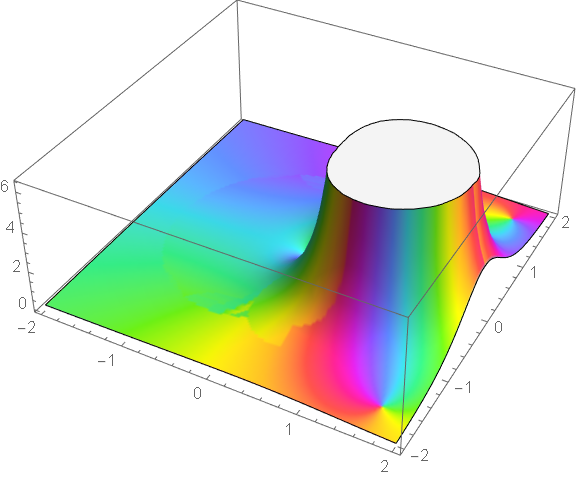
\includegraphics[width=0.75\textwidth]{4.2LHS.png}
 	 	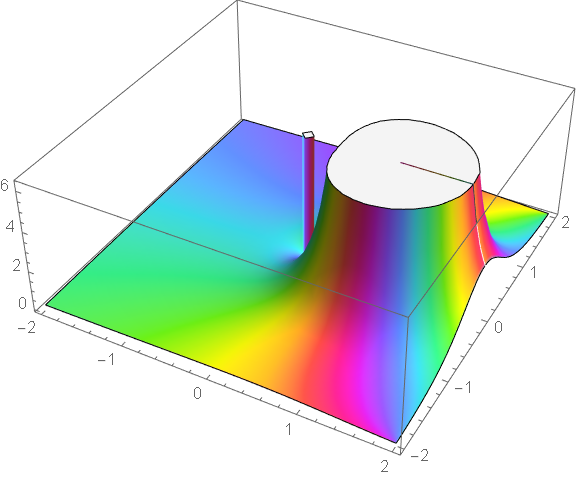
\includegraphics[width=0.75\textwidth]{4.2RHS.png}
 	\caption{The complex plot of the Corollary \ref{4.2.1} for $\mu = \pi + i$, $m=2$, and $n=1$. (Top) The left-hand side of equality. (Bottom) The right-hand side of the equality. For both plots, the $x$-axis refers to the real-part, the $y$-axis define as the imaginary part, the $z$-axis is the absolute value of the expression $\mathrm{Abs}(f)$, and the color refers to the argument of the expression $\mathrm{Arg}(f)$. Both figures generated using Wolfram Mathematica v12.1.}
 	\label{F4.2.1}
 \end{figure}

The above corollary is observe to extends the analyticity outside the region $|z|<1$. This extension is due to the analytic continuation of the function and we can verify it through the complex plot of the equality. Similar to the previous theorem, we plot the left-hand and right-hand side of the equation \eqref{e4.2.1} as a complex plot . This complex plots can be seen in Figure \ref{F4.2.1}. We can see that both plots have a singularity at $z=1$. For the difference of the two plot, we can observe that the right-hand side complex plot has a singularity at $z=0$, which come from the factor $1/z$. Also, it has a branch cut runs along the interval $[1, \infty]$ thas is induce by the hypergeometric function. The manifestation of the branch cut and pole is due to the numerical artifact since Mathematica numerically evaluate the term individually.

\subsubsection{Case $m \leq n$}

When $m \leq n$, all the integrals on the expansion are divergent, and therefore, equation \eqref{mlessn} will hold in this case. The finite part integral is already evaluated in equation \eqref{fp}. Substituting the result to the series, we will have
\begin{equation}
	\begin{split}
	&\sum_{k=0}^{\infty} \, {- n \choose k} \, b^{k} \,\bbint{0}{\infty} \frac{(a+x)^{-\mu}}{x^{k+n-m+1}} \,\mathrm{d}x \\&\hspace{8mm} =  \frac{1 }{a^{n-m+\mu} }\frac{(-1)^{n-m} (n-m+\mu-1)!}{(\mu-1)! (n-m)!} \sum_{k=0}^{\infty} \frac{(n-m+\mu)_k (n)_k}{(n-m+1)_k k!} \\& \hspace{15mm} \times \left[\ln(a)+\psi(k+n-m+1)-\psi(k+n-m+\mu)\right]\left(\frac{b}{a}\right)^k.
	\end{split}
\end{equation}
This is valid for $b/a<1$. Now, we can summed the logarithmic term as a hypergeometric function. This result to
\begin{equation}
\begin{split}
&\sum_{k=0}^{\infty} \, {- n \choose k} \, b^{k} \,\bbint{0}{\infty} \frac{(a+x)^{-\mu}}{x^{k+n-m+1}} \,\mathrm{d}x = \frac{1 }{a^{n-m+\mu} }\frac{(-1)^{n-m} (n-m+\mu-1)!}{(\mu-1)! (n-m)!}\\ &\hspace{4mm}\times\Bigg[\pFq{2}{1}{n-m+\mu,n}{n-m+1}{\frac{b}{a}}\ln(a)  +\sum_{k=0}^{\infty} \frac{(n-m+\mu)_k (n)_k}{(n-m+1)_k k!} \\ &\hspace{16mm} \times [\psi(k+n-m+1)  -\psi(k+m-n+\mu)]\left(\frac{b}{a}\right)^k\Bigg].
\end{split}
\end{equation}
Lastly, for the evaluation of residue, we will use equation \eqref{residue}. Since $n > m$, the term with logarithm for $l = m ,1, ... , n-1$ will just give a zero distribution because of the factor $1/\Gamma(m-k)$
\begin{equation}
\begin{split} 
&\mathrm{Res}  \left[ \frac{z^{m-1} \, (a+z)^{-\mu}}{(b+z)^{n}} \, \log(-z) \right]_{z=-b} 
\\& = \frac{1}{(n-1)!} \sum_{k=0}^{m-1} {n-1 \choose k} \frac{(a-b)^{k-\mu-n+1}}{(-b)^{k-m+1}} \\&\hspace{12mm} \times \frac{\Gamma(1-\mu)}{\Gamma(k-\mu-n+2)}  \frac{\Gamma(m) }{\Gamma(m-k)} \ln(b)  \\& + \frac{1}{(n-1)!} \sum_{k=1}^{n-1} {n -1 \choose k} \, (k-\mu-n+2)_{n-1-k} \, (a-b)^{k-\mu-n+1}\\&\hspace{12mm} \times \sum_{l=1}^{k} {k \choose l} (m-k+l)_{k-l} \frac{\Gamma(l)  (-1)^{l-1}}{(-b)^{k-m+1}}  .
\end{split}
\end{equation}
 Performing some more simplification. we will obtain
\begin{equation}
\begin{split}
   & \mathrm{Res} \, \left[\frac{z^{m-1} \, (a+z)^{-\mu}}{(b+z)^{n}}\, \log(-z) \right]_{z=-b} 
   \\&\hspace{4mm} = \frac{(-1)^{n-m}}{a^{n-m+\mu}} \left(1-b/a\right)^{m-n-\mu} \frac{(n-m+\mu)!(m-1)!}{(\mu-1)!} \\&\hspace{10mm}\times \sum_{l=0}^{m-1}   \frac{(n-m+\mu)_l \ln(b)}{(m-l-1)! (l+n-m)! \,l!} \left(\frac{b/a}{1-b/a}\right)^l
   \\&\hspace{5mm} + \Gamma(m)\Gamma(1-\mu) \sum_{k=1}^{n-1} \sum_{l=1}^{k}  \frac{\Gamma(k-l+1)(-1)^{k-l-m}}{(l)_{1}\Gamma(m-k+l) \Gamma(k-n-\mu+2)  }\\&\hspace{10mm}\times \left( 1-\frac{b}{a} \right)^{k-\mu-n+1} \frac{a^{k-\mu-n+1}}{b^{k-m+1}}.
    \label{residue2}
\end{split}
\end{equation}
Now, gathering all the terms together and substitute them back into equation \eqref{mlessn}, we obtain
\begin{equation}\label{rawresult4b}
\begin{split}
&\frac{\Gamma(m) \Gamma(\mu-m+n)}{\Gamma(\mu+n)}\;\pFq{2}{1}{\mu,m}{\mu+n}{1-\frac{b}{a}}\\
&\hspace{4mm} = \left(\frac{-b}{a}\right)^{n-m} \frac{(n-m+\mu-1)!}{(\mu-1)! (n-m)!}\times\Bigg[\pFq{2}{1}{n-m+\mu,n}{n-m+1}{\frac{b}{a}}\ln(a)  \\ &\hspace{8mm} +\sum_{k=0}^{\infty} \frac{(n-m+\mu)_k (n)_k}{(n-m+1)_k k!} [\psi(k+n-m+1)-\psi(k+n-m+\mu)]\left(\frac{b}{a}\right)^k\Bigg]
\\&\hspace{4mm}- \left(\frac{-b}{a}\right)^{n-m} \left(1-b/a\right)^{m-n-\mu} \frac{(n-m+\mu-1)!(m-1)!}{(\mu-1)!}  \\
   &\hspace{12mm}\times \sum_{l=0}^{m-1} \frac{(n-m+\mu)_l \ln(b)}{(m-l-1)! (l+n-m)! \,l!} \left(\frac{b/a}{1-b/a}\right)^l 
   \\&\hspace{4mm}+ \Gamma(m)\Gamma(1-\mu) \sum_{k=1}^{n-1} \sum_{l=1}^{k}  \frac{\Gamma(k-l+1)(-1)^{k-l-m}}{(l)_{1}\Gamma(m-k+l) \Gamma(k-n-\mu+2)  }
   \\&\hspace{12mm}\times \left( 1-\frac{b}{a} \right)^{k-\mu-n+1} \left( \frac{a}{b}\right)^{k-n+1}.
\end{split}
\end{equation}

Similar to the previous case, we need to show that the coefficient of the logarithm is negative of each other. This will allow as to combine the terms and make the variable all in terms of $b/a$. Starting with the transform from equation \eqref{transform} and applying it to the coefficient of $\ln({a})$, we will have
\begin{equation}
\begin{split}
\sum_{k=0}^{\infty} \frac{(n-m+\mu)_k (n)_k}{(n-m+1)_k k!} z^k &=  \pFq{2}{1}{n-m+\mu,n}{n-m+1}{z}\\
&=(1-z)^{m-n-\mu}\\& \hspace{10mm} \times\pFq{2}{1}{n-m+\mu,1-m}{n-m+1}{\frac{z}{z-1}} .
\end{split}
\end{equation}
Doing the same process from the previous case, the upper parameter $(1-m)$ takes on the value equal to zero or a negative integer. The hypergeometric function in the right-hand side reduces to a polynomial of order $(m-1)$. Expanding and performing the substitutions
\begin{equation}
(1-m)_l = \frac{(-1)^{l}(m-1)!}{(m-l-1)!},\;\;\; (n-m+1)_l = \frac{(l+n-m)!}{(n-m)!}
\end{equation} 
We obtain the equality
\begin{equation}
\begin{split}
&\frac{(n-m+\mu-1)!}{(\mu-1)! (n-m)!} (-1)^{n-m} \sum_{k=0}^{\infty} \frac{(n-m+\mu)_k (n)_k}{(n-m+1)_k k!} z^k \\
&\hspace{4mm} = (1-z)^{m-n-\mu} \frac{(m-1)!(-\mu)!}{(m-n-\mu)!}  \sum_{k=0}^{m-1} \frac{(n-m+\mu)_l}{ (m-l-1)!(l+n-m)! l!} \left(\frac{z}{1-z}\right)^l .
\end{split}
\end{equation}
This allows us to combine the logarithmic terms and by analytic continuation we can replace $b/a$ with the complex variable z. Also, we now lift the restriction that $\mu$ is real. Similar to the previous case, we will rewrite the other infinite series in terms of the function ${}_p\tilde{\psi}_q$ using its definition from equation \eqref{psi}. We obtain the result.
\begin{theorem} \label{4.3}
Let $m$ and $n$ be positive integers with $m<n$, and $\mu$ a complex number with $(\mu-m+n)\neq 0, -1, -2, \dots$. Then
\begin{equation}\label{result4b}
\begin{split}
&\frac{\Gamma(m) \Gamma(\mu-m+n)}{\Gamma(\mu+n)}\;\pFq{2}{1}{\mu,m}{\mu+n}{1-z}\\
&\hspace{4mm} = \left(-z\right)^{n-m} \frac{(n-m+\mu-1)!}{(\mu-1)! (n-m)!} \Bigg[ \pFq{2}{1}{n-m+\mu,n}{n-m+1}{z} \mathrm{Log}(z) \\ 
&\hspace{35mm}  + \pPq{2}{1}{n-m+\mu,n}{n-m+1}{n-m+1}{z}  \\ 
&\hspace{40mm} -\pPq{2}{1}{n-m+\mu,n}{n-m+1}{n-m+\mu}{z} \Bigg]
   \\&\hspace{4mm}+ \sum_{k=1}^{n-1} \sum_{l=1}^{k}  \frac{\Gamma(m)\Gamma(1-\mu)\Gamma(k-l+1)(-1)^{k-l-m}}{z^{-\mu}(l)_{1}\Gamma(m-k+l) \Gamma(k-n-\mu+2)}  \left( \frac{1-z}{z} \right)^{k-\mu-n+1}.
\end{split}
\end{equation}
for all $z\not=1$ and $|\mathrm{arg}(z)|<\pi$. All the functions involve are taken as their principal value. 
\end{theorem}
\noindent The above equality looks like a new identity of the Gauss hypergeometric function.

Similar to the previous case, we will now exploit the hypergeometric-type series containing the digamma function to generate a reduction formula of the Kampé de Fériet function. Using the relation in equation \eqref{DxK}, we can construct the following relations:
\begin{align}
\begin{split}
    \pPq{2}{1}{n-m+\mu,n}{n-m+1}{n-m+1}{z} &\\&\hspace{-50mm} =  \psi(n-m+1) \, \pFq{2}{1}{n-m+\mu,n}{n-m+1}{z} + z\, \frac{(n-m+\mu) \, n}{n-m+1} \\& \hspace{-45mm} \times  F^{2 \, 1 \, 2}_{2 \, 0 \, 1}\left[\begin{array}{lll}
	n-m+\mu+1, n+1 &: 1 &; 1,n-m+1  \\
	2, n-m+2&:  &; n-m+2 
	\end{array};\; z,z\right]
\end{split}
\end{align}
and
\begin{align}
\begin{split}
    \pPq{2}{1}{n-m+\mu,n}{n-m+1}{n-m+\mu}{z} &\\&\hspace{-50mm} = \psi(n-m+\mu) \, \pFq{2}{1}{n-m+\mu,n}{n-m+1}{z}  + z\, \frac{ \, n}{n-m+1} \\& \hspace{-45mm} \times F^{2 \, 1 \, 2}_{2 \, 0 \, 1}\left[\begin{array}{lll}
	n-m+\mu+1, n+1 &: 1 &; 1,n-m+\mu  \\
	2, n-m+2&:  &; n-m+\mu+1 
	\end{array};\; z,z\right].
\end{split}
\end{align}

Using the above relation and expressing the infinite series as a hypergeometric function, we will obtain a corollary of theorem \ref{4.3}. 

\begin{corollary} \label{4.3.1e}
Let $m$ and $n$ be positive integers with $m>n$, and $\mu$ a complex number with $(\mu-m+n)\neq 0, -1, -2, \dots$. Then
	\begin{equation}
	\begin{split}\label{4.3.1}
    F^{2 \, 1 \, 2}_{2 \, 0 \, 1}&\left[\begin{array}{lll}
	n-m+\mu+1, n+1 &: 1 &; 1,n-m+\mu  \\
	2, n-m+2&:  &; n-m+\mu+1 
	\end{array};\; z,z\right] \\& \hspace{-10mm} - (n-m+\mu) \, F^{2 \, 1 \, 2}_{2 \, 0 \, 1}\left[\begin{array}{lll}
	n-m+\mu+1, n+1 &: 1 &; 1,n-m+1  \\
	2, n-m+2&:  &; n-m+2 
	\end{array};\; z,z\right] \\& \hspace{5mm} =
	 \frac{n-m+1}{z \, n} \pFq{2}{1}{n-m+\mu,n}{n-m+1}{z} 
	\\& \hspace{15mm} \times \left[ \psi(n-m+1) -\psi(n-m+\mu) - \mathrm{Log}(z) \right] 
   \\&\hspace{10mm}- \frac{\Gamma(\mu) (n-m+1)! (-1)^{m-n}}{\Gamma(n+\mu) \, n \,z^{n-m+1}} \pFq{2}{1}{\mu,m}{\mu+n}{1-z}
   \\&\hspace{10mm}+ \frac{\Gamma(m)\Gamma(\mu)\Gamma(1-\mu)(n-m+1)!}{\Gamma(n-m+\mu) \,n \, z^{n-m-\mu+1} } \\& \hspace{15mm} \times \sum_{k=1}^{n-1}  \sum_{l=1}^{k}  \frac{\Gamma(k-l+1)(-1)^{k-l-n}}{(l)_{1}\Gamma(m-k+l) \Gamma(k-n-\mu+2)} \left( \frac{1-z}{z} \right)^{k-\mu-n+1}.
	\end{split}
	\end{equation}
	for all $z \not = 1$ and $|\mathrm{arg}(z)|<\pi$.
 All the functions involve are taken as their principal value. \end{corollary} 

\begin{figure}[t]
 	\centering
 	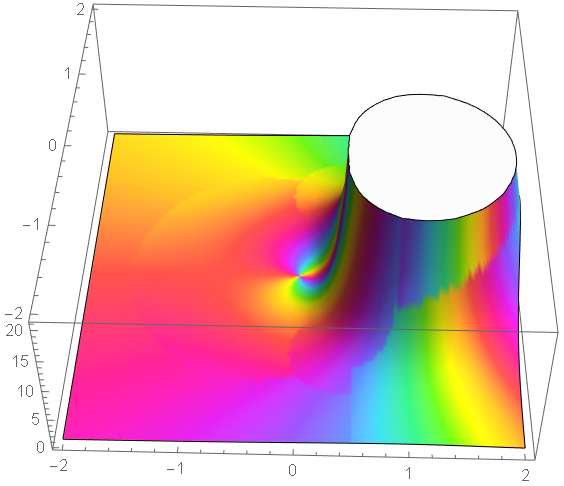
\includegraphics[width=0.75\textwidth]{4.3LHS.png}
 	 	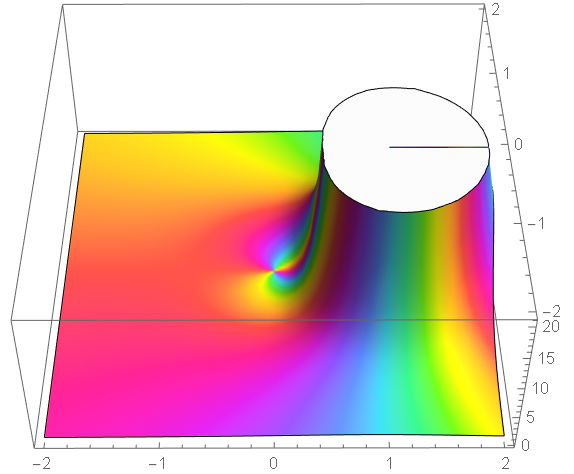
\includegraphics[width=0.75\textwidth]{4.3RHS.png}
 	\caption{The complex plot of the Corollary \ref{4.3.1} for $\mu = \pi + i$, $m=1$ and $n=3$. (Top) The left-hand side of equality. (Bottom) The right-hand side of the equality. For both plots, the $x$-axis refers to the real-part, the $y$-axis define as the imaginary part, the $z$-axis is the absolute value of the expression $\mathrm{Abs}(f)$, and the color refers to the argument of the expression $\mathrm{Arg}(f)$. Both figures generated using Wolfram Mathematica v12.1.}
 	\label{F4.3.1}
 \end{figure}

The above result appears to extend the analyticity outside the region of $|z| < 1$ by the principle of analytic continuation. Again, for accuracy check, we will obtain the complex plot of the left-hand and right-hand side of the equation \eqref{4.3.1e}. From Figure \ref{F4.3.1}, we can see that the complex plot for both sides seems identical too. Both figures is observed to have a zero at $z=0$ and singularity at $z=1$. The only difference we observe is the branch cut along $[1, \infty]$, which is due to the hypergeometric function. Again, the appearance of the branch cut for the complex plot of the right hand side equation is due to the numerical artifacts of the numerical evaluation. 


\subsubsection{Special case: $m = 1$}

If we let $ m = 1$, the Stieltjes transform in equation \eqref{STGHF} will reduce to
\begin{equation}
\int_0^{\infty} \frac{(a+x)^{-\mu}}{(b+x)^{n}} \, \mathrm{d}x = \frac{ \Gamma(\mu+n-1)}{\Gamma(\mu+n)} \frac{b^{1-n}}{a^{\mu}}\, \pFq{2}{1}{\mu,1}{\mu+n}{1-\frac{b}{a}}. 
\label{STGHF}
\end{equation}
Since $m,n$ are positive integers, this special case will always fall under the case of $n \geq m$. Invoking the corollary \ref{4.3.1} and simplifying terms, we will have a reduction formula 
\begin{equation}
	\begin{split} \label{5.64}
    F^{1 \, 1 \, 2}_{1 \, 0 \, 1}&\left[\begin{array}{lll}
	n+\mu &: 1 &; 1,n+\mu-1  \\
	2 &:  &; n+\mu 
	\end{array};\; z,z\right] \\& \hspace{-10mm} - (n+\mu-1) \, F^{1 \, 1 \, 2}_{1 \, 0 \, 1}\left[\begin{array}{lll}
	n+\mu &: 1 &; 1,n  \\
	2&:  &; n+1 
	\end{array};\; z,z\right] \\& \hspace{5mm} =
	 \frac{1}{z} \pFq{1}{0}{n+\mu-1}{}{z} 
	\\& \hspace{20mm} \times \left[ \psi(n) -\psi(n+\mu-1) - \mathrm{Log}(z) \right] 
   \\&\hspace{10mm}- \frac{\Gamma(\mu) (n-1)! (-1)^{1-n}}{\Gamma(n+\mu) \,z^{n}} \pFq{2}{1}{\mu,1}{\mu+n}{1-z}
      \\&\hspace{10mm}+ \frac{\Gamma(\mu)\Gamma(1-\mu)(n-1)!}{\Gamma(n+\mu-1) \, z^{n-\mu} } \\& \hspace{20mm} \times \sum_{k=1}^{n-1}  \frac{(-1)^{1-n}}{k\Gamma(n-k)\Gamma(2-\mu-n+k)} \left( \frac{1-z}{z} \right)^{k-\mu-n+1}.
	\end{split}
	\end{equation}
According to \cite{ancarani2010derivatives}, we can express the Kampé de Fériet function as a differentation of the hypergeometric function with respect to the parameter. Letting $\alpha = n+\mu-1$, the first term of the left hand side can be express as
\begin{equation}
	\begin{split}
    F^{1 \, 1 \, 2}_{1 \, 0 \, 1} \left[\begin{array}{lll}
	\alpha+1 &: 1 &; 1,\alpha  \\
	2 &:  &; \alpha +1
	\end{array};\; z,z\right] & = \frac{\partial }{\partial \alpha} \frac{1}{z} \pFq{1}{0}{\alpha}{}{z}
	\\& = \frac{1}{z} \frac{\partial }{\partial \alpha}  (1-z)^{-\alpha}
	\\& = - \frac{1}{z} \ln{(1-z)} (1-z)^{\alpha}
	\\& = - \frac{1}{z} \ln{(1-z)} \pFq{1}{0}{\alpha}{}{z}.
	\end{split}
	\end{equation}
Substituting the above expression to equation \eqref{5.64}, we will result to
\begin{equation}
	\begin{split} \label{SPP}
     F^{1 \, 1 \, 2}_{1 \, 0 \, 1}&\left[\begin{array}{lll}
	n+\mu &: 1 &; 1,n  \\
	2&:  &; n+1 
	\end{array};\; z,z\right] \\& \hspace{5mm} =
	- \frac{1}{z (n+\mu-1)} \pFq{1}{0}{n+\mu-1}{}{z} 
	\\& \hspace{20mm} \times \left[ \mathrm{Log} \left( \frac{1-z}{z} \right) + \psi(n) -\psi(n+\mu-1) \right] 
   \\&\hspace{10mm}+ \frac{\Gamma(\mu) (n-1)! (-1)^{1-n}}{\Gamma(n+\mu) (n+\mu-1) \,z^{n}} \pFq{2}{1}{\mu,1}{\mu+n}{1-z}
      \\&\hspace{10mm}- \frac{\Gamma(\mu)\Gamma(1-\mu)(n-1)!}{\Gamma(n+\mu) \, z^{n-\mu} } \\& \hspace{20mm} \times \sum_{k=1}^{n-1}  \frac{(-1)^{1-n}}{k\Gamma(n-k)\Gamma(2-\mu-n+k)} \frac{(1-z)^{k-\mu-n+1}}{z^{k+1}} .
	\end{split}
	\end{equation}
The above expression is just the reduction formula of the Kampé de Fériet function found in  \cite{SPP-2020-2G-03}. We create a $3$D plot of the left-hand side and right-hand side of the equation for some accuracy checks. It can be seen in Figure \ref{FSPP} that the plot of both expression have a singularity at $z = 1$ and look the same. The only difference is the two branch cuts on the right hand side plot due to the numerical artifacts of the logarithmic term. The plots confirm the accuracy of the above equation.

\begin{figure}[t]
 	\centering
 	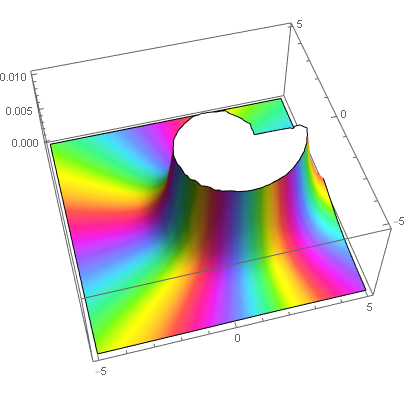
\includegraphics[width=0.6\textwidth]{SPPLHSf.png}
 	 	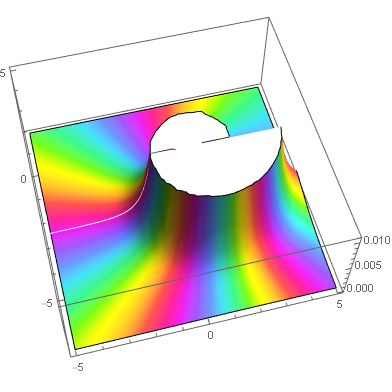
\includegraphics[width=0.6\textwidth]{SPPRHSf.png}
 	\caption{The complex plot of the equation \eqref{SPP} for $\mu = \pi + i$ amd $n=3$. (Top) The left-hand side of equality. (Bottom) The right-hand side of the equality. For both plots, the $x$-axis refers to the real-part, the $y$-axis define as the imaginary part, the $z$-axis is the absolute value of the expression $\mathrm{Abs}(f)$, and the color refers to the argument of the expression $\mathrm{Arg}(f)$. Both figures generated using Wolfram Mathematica v12.1.}
 	\label{FSPP}
 \end{figure}


\subsection{Case 2: $\nu$, $\rho \not \in \mathbb{Z}^{+}$, $\nu-\rho \in \mathbb{Z}$}

We will consider here the case $\mu, \nu, \rho > 0$, and $\nu,\rho \not \in \mathbb{Z}^{+}$. The origin $z=0$ is pole singularity when the difference of $(\nu-\rho)$ is an integer and $z=-b$ is a branch point since $\rho$ is not an integer. We choose the branch cut to run along the positive real axis. Now, we will extract the desired integral from the contour integral 
\begin{equation}
\int_C \frac{z^{\nu-1} (a+z)^{-\mu}}{(b+z)^{\rho}}\,\left(\log z - i\pi\right)\, \mathrm{d}z,
\end{equation}
since the divergence is from a pole singularity. The contour $C$ is shown in Figure \ref{deformation} and will be collapsed into $C'$. The $C'$ contour is evaluated as  
\begin{equation}
\begin{split}
&\int_0^{\infty} \frac{x^{\nu-1} (a+x)^{-\mu}}{(b+x)^{\rho}} \mathrm{d}x=  \frac{1}{2\pi i} \int_C \frac{z^{\nu-1} (a+z)^{-\mu}}{(b+z)^{\rho}}\,\left(\log z - i\pi\right)\, \mathrm{d}z \\
& \hspace{24mm}+ (-1)^{\nu-\rho+1} \frac{\sin(\pi \rho)}{\pi} \lim_{\epsilon\rightarrow 0} \left[\int_0^{b-\epsilon} \frac{x^{\nu-1} (a-x)^{-\mu}}{(b-x)^{\rho}}\,\log(x)\,\mathrm{d}x \right. \\
& \hspace{24mm}\left.  + \frac{e^{-i\pi\nu}}{(1-e^{-2\pi\rho i})}\int_{C_{\epsilon}} \frac{z^{\nu-1} (a+z)^{-\mu}}{(b+z)^{\rho}}\,\left(\log z - i\pi\right)\, \mathrm{d}z\right].
\end{split}
\end{equation}
Again, we recognize that the limit is the finite part of the divergent integral $\int_0^b x^{\nu-1} (a+x)^{-\mu} (b+x)^{-\rho}\,\mathrm{d}x$. Then, the representation reduces to 
\begin{equation}
\begin{split} \label{repcase4b}
&\int_0^{\infty} \frac{x^{\nu-1} (a+x)^{-\mu}}{(b+x)^{\rho}}\mathrm{d}x =  \frac{1}{2\pi i} \int_C \frac{z^{\nu-1} (a+z)^{-\mu}}{(b+z)^{\rho}}\,\left(\log z - i\pi\right)\, \mathrm{d}z \\
& \hspace{24mm}+  (-1)^{\nu-\rho+1}\frac{\sin(\pi\rho)}{\pi} \bbint{0}{b} \frac{x^{\nu-1} \, (a-x)^{-\mu}}{(b-x)^{\rho}} \, \ln(x)\, \mathrm{d}x.
\end{split}
\end{equation}
The equality holds for $a>b>0$, $\mathrm{Re}(\nu) > 0$, $\mathrm{Re}(\rho) > 0$ , $\mu \not = 0$, $(\rho+\mu-\nu)>0$, $\rho \not \in \mathbb{Z}$ and $(\nu-\rho)\in \mathbb{Z}$. Next, we will perform the same expansion in the first term and perform a term by term integration. Similar to the previous case, there are two possible cases, depending on whether all the integrals appearing are finite-part integrals or not. Also, the third term introduces two possible cases depending on the value of $\rho$: If $0<\rho<1$, the integral is just a regular convergent integral; if $\rho\geq 1$, the integral is the finite part of a divergent integral. Nevertheless, we can simultaneously consider the two cases because the finite part coincides with the regular value of the integral when it converges. 

Let us now obtain the finite part integral in equation \eqref{repcase4b}. To determine the convergent and divergent parts of the integral, we let $\epsilon$ be some positive arbitrarily small number and consider the integral
\begin{equation}
\frac{a^{\mu}}{b^{\nu-\rho}}\int_{0}^{b-b\epsilon} \frac{x^{\nu-1} (a-x)^{-\mu}}{(b-x)^{\rho}}\,\ln(x)\, \mathrm{d}x = C_{\epsilon} + D_{\epsilon}.
\end{equation}
In the limit as $\epsilon$ approaches zero, the $C_{\epsilon}$ and $D_{\epsilon}$ are the convergent and divergent parts, respectively. Recall that the assigned finite part is the limit $\lim_{\epsilon\rightarrow 0} C_{\epsilon}$. Performing some change in variable $x=b y$ will reduce the integral into
\begin{equation}\label{integralorig}
\begin{split}
&\frac{a^{\mu}}{b^{\nu-\rho}}\int_0^{b-b\epsilon} \frac{x^{\nu-1} (a-x)^{-\mu}}{(b-x)^{\rho}}\,\ln(x)\, \mathrm{d}x =  \ln(b) \int_0^{1-\epsilon} \frac{y^{\nu-1} (1-\frac{b}{a} y)^{-\mu}}{(1-y)^{\rho}}\, \mathrm{d}y \\
& \hspace{20mm}+\int_0^{1-\epsilon} \frac{y^{\nu-1} \left(1-\frac{b}{a} y\right)^{-\mu}}{(1-y)^{\rho}}\,\ln(y)\,\mathrm{d}y,
\end{split}
\end{equation}
for $b>0$. The above expression will result to a combination of two finite part integrals,
\begin{equation}\label{integralorigx}
\begin{split}
&\frac{a^{\mu}}{b^{\nu-\rho}}\bbint{0}{b} \frac{x^{\nu-1} (a-x)^{-\mu}}{(b-x)^{\rho}}\,\ln(x)\, \mathrm{d}x =  \ln(b) \bbint{0}{1} \frac{y^{\nu-1} (1-\frac{b}{a} y)^{-\mu}}{(1-y)^{\rho}}\, \mathrm{d}y \\
& \hspace{20mm}+\bbint{0}{1} \frac{y^{\nu-1} \left(1-\frac{b}{a} y\right)^{-\mu}}{(1-y)^{\rho}}\,\ln(y)\,\mathrm{d}y .
\end{split}
\end{equation}
The two finite-part integral in the right hand side can be generalized as \begin{equation}
\int_0^{1-\epsilon} \frac{y^{\nu-1} (1-\frac{b}{a} y)^{-\mu}}{(1-y)^{\rho}}\,g_l(y) \mathrm{d}y = C_{\epsilon}^{(l)} + D_{\epsilon}^{(l)}, \;\;\; l=1, 2, 
\end{equation}
where $g_1(y)=1$ and $g_2(y)=\ln(y)$, and the  $C_{\epsilon}^{(l)}$'s and $D_{\epsilon}^{(l)}$'s are the respective converging and diverging parts of the integrals. For the evaluation of this integrals, we let $b/a<(1-\epsilon)$ and expand $(1-b y/a)^{-\mu}$ at the origin. Then, we will interchange the order of integral and summation to perform a term by term integration. The interchanging of the operators is allowed since the series is uniformly convergent along the interval of integration $[0,1-\epsilon]$,
\begin{align}
\begin{split}
    \int_0^{1-\epsilon} & \frac{y^{\nu-1} (1-\frac{b}{a} y)^{-\mu}}{(1-y)^{\rho}} \,g_l(y)\,  \mathrm{d}y \\& = \sum_{k=0}^{\infty} (-1)^k {-\mu \choose k}\left(\frac{b}{a}\right)^k \int_0^{1-\epsilon} \frac{y^{\nu-1+k}}{(1-y)^{\rho}}\,g_l(y)\,\mathrm{d}y.    
\end{split}
\end{align}
This lead us to evaluate the integrals
\begin{equation}\label{rawintegral}
\int_0^{1-\epsilon} \frac{y^{\nu+k-1}}{(1-y)^{\rho}}\,g_l(y)\,\mathrm{d}y=\tilde{C}^{(l)}_{k,\epsilon} + \tilde{D}^{(l)}_{k,\epsilon},
\end{equation}
where the $\tilde{C}^{(l)}_{\epsilon}$'s and $\tilde{D}^{(l)}_{\epsilon}$'s are the converging and diverging parts of the integrals for a given $k$. The converging parts of $C_{\epsilon}$ will obviously come from the converging parts of $\tilde{C}_{k,\epsilon}$'s. Therefore, when the infinite series converges, the finite integrals are given by
\begin{equation}\label{fpixxx}
\bbint{0}{1}\frac{y^{\nu-1} (1-\frac{b}{a} y)^{-\mu}}{(1-y)^{\rho}}\, \mathrm{d}y = \sum_{k=0}^{\infty} (-1)^k {-\mu \choose k}\left(\frac{b}{a}\right)^k \bbint{0}{1} \frac{y^{\nu-1+k}}{(1-y)^{\rho}}\,\mathrm{d}y ,
\end{equation}
\begin{equation}\label{fpixxx2}
\bbint{0}{1}\frac{y^{\nu-1} (1-\frac{b}{a} y)^{-\mu}}{(1-y)^{\rho}}\,\ln(y)\, \mathrm{d}y = \sum_{k=0}^{\infty} (-1)^k {-\mu \choose k}\left(\frac{b}{a}\right)^k \bbint{0}{1} \frac{y^{\nu-1+k}}{(1-y)^{\rho}}\,\ln(y)\,\mathrm{d}y.
\end{equation}
The task now is evaluate this two finite-part integrals
\begin{equation}
\bbint{0}{1} \frac{y^{\nu-1+k}}{(1-y)^{\rho}}\,\mathrm{d}y,\;\;\;
%\end{equation}
%\begin{equation}
\bbint{0}{1} \frac{y^{\nu-1+k}}{(1-y)^{\rho}}\,\ln(y)\,\mathrm{d}y.
\end{equation}
Observe that the only difference between the two finite-part integrals is the logarithmic factor and this factor can be generated through differentiation. Hence, the second finite-part integrals can be obtained from the differentiation of the first finite-part integral. 

To evaluate the first finite-part integral, we will consider the finite-part integral 
\begin{equation}
\bbint{0}{1}\frac{y^{\sigma-1}}{(1-y)^{\rho}}\,\mathrm{d}y.
\end{equation}
where $\mathrm{Re}(\sigma)>0$ and $\mathrm{Re}(\rho)>0$. Then, we consider the usual integral 
\begin{equation} \label{fp1}
\int_0^{1-\epsilon} \frac{y^{\sigma-1}}{(1-y)^{\rho}}\,\mathrm{d}y
\end{equation} 
where $0<\epsilon<1$. To completely evaluate the above integral, we will use the two facts about beta function $B(a,b)$, its integral representation
\begin{equation}\label{betaintegrep}
B_{z}(a,b) = \int_0^z t^{a-1} (1-t)^{b-1}\,\mathrm{d}t,\; \mathrm{Re}(a)>0,
\end{equation}
and its behavior in the neighbhood of $z=1$.
\begin{equation}\label{betainc1}
B_z(a,b)= B(a,b) - \frac{(1-z)^{b} z^a}{b}\left(1+O(z-1)\right),
\end{equation}
Comparing the integral \eqref{fp1} from the integral representation of Beta function in \eqref{betaintegrep}, we will obtain the integral \eqref{fp1} as the incomplete beta function with $z=1-\epsilon$, $a=\sigma$ and $b=1-\rho$
\begin{equation} \label{fp12}
    \int_{0}^{1-\epsilon} \frac{y^{\sigma-1}}{(1-y)^{\rho}} \,\mathrm{d}y = B_{1-\epsilon}(\sigma, 1-\rho).
\end{equation}
Then, invoking the expansion of the beta funtion \eqref{betainc1} at $z=1$, the integral \eqref{fp12} will results to
\begin{align}
    \int_0^{1-\epsilon} \frac{y^{\sigma-1}}{(1-y)^{\rho}}\,\mathrm{d}y & = B(\sigma, 1-\rho) - \frac{\epsilon^{1-\rho} (1-\epsilon)^{\sigma}}{1-\rho} + \left(1+O(-\epsilon)\right)
    \\& =\frac{\pi\Gamma(\sigma)}{\sin(\pi\rho) \Gamma(\rho) \Gamma(1+\sigma-\rho)} + O(\epsilon^{1-\rho}),
\end{align}
where we made a further simplification using the fact that $\rho$ is a non-integer. If $\mathrm{Re}(\rho)<1$, the second term will just approach to zero as $\epsilon \to 0$. It implies that the finite-part integral is a converging integral, and it will just take its value. While, when $\mathrm{Re}(\rho)>1$, the second term will diverge. In this case, the finite-part integral will be obtained by dropping the diverging part and performing the limit $\epsilon \to 0$ to the converging part. Thus we arrive at the finite part integral
\begin{equation}\label{fpingteg1x}
\bbint{0}{1}\frac{y^{\sigma-1}}{(1-y)^{\rho}}\,\mathrm{d}y = \frac{\pi\Gamma(\sigma)}{\sin(\pi\rho) \Gamma(\rho) \Gamma(1+\sigma-\rho)},
\end{equation}
for $\mathrm{Re}(\sigma)>0$ and $\mathrm{Re}(\rho)>0$. Since $1/\Gamma(z)=0$ for $z \in \mathbb{Z}_{0}^{-}$, the finite part assumes the zero value for $1+\sigma-\rho\in \mathbb{Z}_{0}^{-}$. Explicitly, we have
\begin{equation}\label{fpingteg1xxx}
\bbint{0}{1}\frac{y^{\sigma-1}}{(1-y)^{\rho}}\,\mathrm{d}y = 0,
\end{equation}
for $\sigma - \rho \in \mathbb{Z}_{0}^{-}$.

For the calculation of the second finite-part integral, we will perform some classic Feymann tricks. Inspecting the integral, we can see that that the integral the two integral is related by some differentiation of the parameter. Using the fact that 
\begin{equation}
    \frac{\partial}{\partial \nu} y ^{\nu-1} =  y^{\nu-1}\, \ln{y} \
\end{equation}
we can establish the following relation
\begin{equation}
    \frac{\partial}{\partial\nu} \, \int_0^{1-\epsilon}  \frac{y^{\nu-1}} {(1-y)^{\rho}}\,\mathrm{d}y =  \int_0^{1-\epsilon}  \frac{y^{\nu-1}} {(1-y)^{\rho}} \ln y \,\mathrm{d}y. 
\end{equation}
This relation confirms by the converges of the integral along the entire integration interval $[0,1-\epsilon]$. Therefore, the second finite part in the right hand side of equation \eqref{integralorigx} is just the differentiation with respect to $\nu$ of the finite-part integral \eqref{fpingteg1x}. Performing the differentiation on equation \eqref{fpingteg1x}, we obtain the second finite-part integral as
\begin{equation}\label{fpingteg1xxx2}
\bbint{0}{1}\frac{y^{\sigma-1}}{(1-y)^{\rho}}\,\ln(y)\,\mathrm{d}y = \frac{\pi\Gamma(\sigma)}{\sin(\pi\rho) \Gamma(\rho) \Gamma(1+\sigma-\rho)} \left(\psi(\sigma)-\psi(\sigma-\rho+1)\right),
\end{equation}
for $\mathrm{Re}(\sigma)>0$ and $\mathrm{Re}(\rho)>0$ and non-integer $\rho$. For $\sigma-\rho+1 \in \mathbb{Z}_{0}^{-}$, we will have a removable singularity  
\begin{equation}
    \lim_{z\rightarrow -n} \frac{\psi(z)}{\Gamma(z)} = (-1)^{n+1} n!,
\end{equation}
for a positive integer $n$. This yields the finite part integral
\begin{equation}\label{fpingteg1xx3}
\bbint{0}{1}\frac{y^{\sigma-1}}{(1-y)^{\rho}}\,\ln(y)\,\mathrm{d}y = (-1)^{\rho-\sigma+1} \frac{\pi\Gamma(\sigma) (\rho-\sigma-1)!}{\sin(\pi\rho) \Gamma(\rho)},
\end{equation}
for $(\sigma-\rho) \in \mathbb{Z}_{0}^{-}$.

Inspecting all the finite-part integral, it is observed that all finite-part integral depends on the difference of the parameters $\rho$ and $\nu$. Thus,  we will consider separately the cases $(\nu-\rho) \in \mathbb{Z}^{+}$ and $(\rho-\nu) \in \mathbb{Z}_{0}^{-}$.  

\subsubsection{Case $(\nu-\rho) \in \mathbb{Z}^{+}$}

For this case, the expansion in the equation \eqref{repcase4b} decomposes into a finite series of convergent integrals and an infinite series of finite part integrals. The expansion assumes the form
\begin{equation}
\begin{split} 
\int_0^{\infty} \frac{x^{\nu-1} (a+x)^{-\mu}}{(b+x)^{\rho}} \mathrm{d}x  = &  \sum_{k=0}^{(\nu-\rho)-1} \, {- \rho \choose k} \, b^{k} \int_0^{\infty} \ \frac{(a+x)^{-\mu}}{x^{k+\rho-\nu+1}} \,\mathrm{d}x \\& + \sum_{k=(\nu-\rho)}^{\infty} {- \rho \choose k} \, b^{k} \, \bbint{0}{\infty} \frac{(a+x)^{-\mu}}{x^{k+\rho-\nu+1}} \,\mathrm{d}x
\\&- (-1)^{\nu-\rho}\frac{\sin(\pi\rho)}{\pi} \bbint{0}{b} \frac{x^{\nu-1} \, (a-x)^{-\mu}}{(b-x)^{\rho}} \, \ln(x)\, \mathrm{d}x.
\label{case4b}
\end{split}
\end{equation}
From the definition of beta function, the integrals in the first group of terms evaluate to
\begin{equation}
    \int_0^{\infty} \frac{(a+x)^{-\mu}}{x^{k+\rho-\nu+1}}\,\mathrm{d}x = \frac{\Gamma(\nu-\rho-k)\Gamma(k+\mu-\nu+\rho)}{a^{k+\mu+\nu-\rho} \Gamma(\mu)},
\end{equation}
for $k=0, \dots, (\nu-\rho-1)$. On the other hand, the finite part integrals in the second term is given by the equation \eqref{fp} with the substitution $n-m \to \rho-\nu$. This will give us
\begin{equation}
\begin{split} \label{second}
    \bbint{0}{\infty} \frac{(a+x)^{-\mu}}{x^{k+\rho-\nu+1}} \,\mathrm{d}x &= \frac{1}{a^{k+\rho-\nu+\mu}} {-\mu \choose k+\rho-\nu} \\
    &\times\left[\ln(a) + \psi(k+\rho-\nu+1)-\psi(k+\rho-\nu+\mu)\right]
    \end{split}
\end{equation}
for $=(\nu-\rho), (\nu-\rho+1),\dots$. We can now further simplify this two group terms of equation \eqref{case4b}. Substituting the values of the convergent integrals, the first term will become
\begin{equation}\label{xxx1}
\begin{split}
    &\sum_{k=0}^{(\nu-\rho)-1} \, {- \rho \choose k} \, b^{k} \int_0^{\infty} \ \frac{(a+x)^{-\mu}}{x^{k+\rho-\nu+1}} \,\mathrm{d}x \\
    &\hspace{8mm}= \frac{1}{a^{\mu-\nu+\rho} \Gamma(\mu)} \sum_{k=0}^{\nu-\rho-1} {-\rho \choose k} \Gamma(\nu-\rho-k) \Gamma(k+\mu-\nu+\rho) \left(\frac{b}{a}\right)^k
    \end{split}
\end{equation}
Writing the binomial coefficient in terms of the gamma function and using the identity $\Gamma(z-n) = (-1)^{n} \Gamma(z)/(1-z)_n$, the right hand side of equation simplifies to
\begin{equation}\label{xxx1v2}
\begin{split}
    &\sum_{k=0}^{(\nu-\rho)-1} \, {- \rho \choose k} \, b^{k} \int_0^{\infty} \ \frac{(a+x)^{-\mu}}{x^{k+\rho-\nu+1}} \,\mathrm{d}x \\
    &\hspace{8mm}= \frac{\Gamma(\nu-\rho) \Gamma(\mu-\nu+\rho)}{a^{\mu+\rho-\nu}\Gamma(\mu)} \sum_{k=0}^{\nu-\rho-1} \frac{(\rho)_k (\mu-\nu+\rho)_k}{(1-\nu+\rho)_k k!} \left(\frac{b}{a}\right)^k.
       \end{split}
\end{equation}
For the second group of terms, we substitute the evaluated finite part integrals in equation \eqref{second}. Next is to shift the index of summation from $k$ to $k+\nu-\rho$ so that we can easily transform it into a hypergeometric function. Then, we write all binomial coefficients in terms of the gamma function. This will result to
\begin{equation}
    \begin{split} \label{xxx2}
        &\sum_{k=(\nu-\rho)}^{\infty} {- \rho \choose k} \, b^{k} \, \bbint{0}{\infty} \frac{(a+x)^{-\mu}}{x^{k+\rho-\nu+1}} \,\mathrm{d}x\\
        &\hspace{4mm}= 
    \frac{b^{\nu-\rho}}{a^{\mu}} \frac{(-1)^{\nu-\rho}}{\Gamma(\mu) \Gamma(\rho)} \sum_{k=0}^{\infty} \frac{\Gamma(k+\mu) \Gamma(k+\nu)}{\Gamma(k+\nu-\rho+1) k!} \\& \hspace{10mm} \times \left[\ln{a}+\psi(k+1)-\psi(k+\mu)\right]\left(\frac{b}{a}\right)^k.
    \end{split}
\end{equation}
The infinite series converges for all $|b/a|<1$ and $\mathrm{Re}(\rho-\nu+\mu)>0$.

Finally, we evaluate the last term of equation \eqref{case4b}. Under the condition that $(\nu-\rho)$ is a positive integer, and with $\sigma=\nu+k$, the finite-part integral \eqref{fpingteg1x} does not vanish for all $k=0, 1, \dots$. Substituting the finite parts \eqref{fpingteg1x} back into equation \eqref{fpixxx} yields 
\begin{equation}\label{integralseries}
    \bbint{0}{1} \frac{y^{\nu-1} (1-\frac{b}{a} y)^{-\mu}}{(1-y)^{\rho}}\, \mathrm{d}y =\frac{\pi}{\sin(\pi\rho)\Gamma(\mu)\Gamma(\rho)}\sum_{k=0}^{\infty} \frac{\Gamma(k+\mu) \Gamma(k+\nu)}{\Gamma(1+k+\nu-\rho) k!} \left(\frac{b}{a}\right)^k ,
\end{equation}
for $b/a<1$, where the binomial coefficient has been written in terms of the gamma function to arrive at this expression. To extend the result to accommodate the case $b/a>1$, we perform a hypergeometric summation to the infinite series to give  
\begin{equation}\label{integralclosed}
    \bbint{0,}{1} \frac{y^{\nu-1} (1-\frac{b}{a} y)^{-\mu}}{(1-y)^{\rho}}\, \mathrm{d}y= \frac{\pi \Gamma(\nu)}{\sin(\pi \rho) \Gamma(\rho) \Gamma(1+\nu-\rho)} \, \pFq{2}{1}{\mu,\nu}{1+\nu-\rho}{\frac{b}{a}} ,
\end{equation}

Similarly the finite part integral is given by equation \eqref{fpingteg1xx3} for all $k$. Then substituting the finite part into equation, the logarithmic finite part integral is given by
\begin{equation}\label{integrallogseries}
\begin{split}
    &\bbint{0}{1} \frac{y^{\nu-1} (1-\frac{b}{a} y)^{-\mu}}{(1-y)^{\rho}}\,\ln(y)\, \mathrm{d}y=\frac{\pi}{\sin(\pi\rho) \Gamma(\mu)\Gamma(\rho)} \\ 
    &\hspace{18mm}\times\sum_{k=0}^{\infty} \frac{\Gamma(k+\mu) \Gamma(k+\nu)}{\Gamma(1+k+\nu-\rho) k!}  \left[\psi(k+\nu)-\psi(1+k+\nu-\rho)\right] \left(\frac{b}{a}\right)^k ,
    \end{split}
\end{equation}
for $\rho>1$ or the regular value when $\rho<1$; this result is valid for $b/a<1$. The extension of this result for $b/a>1$ can be obtained by differentiating equation \eqref{integralclosed} with respect to $\nu$.

Again, the two finite-part integral above are the finite-part of the singular contribution. Substituting those finite part to the equation \eqref{integralorigx} will result to
\begin{equation}
\begin{split}
&\frac{a^{\mu}}{b^{\nu-\rho}} \bbint{0}{b} \frac{x^{\nu-1} \, (a-x)^{-\mu}}{(b-x)^{\rho}} \, \ln(x)\, \mathrm{d}x\\
&\hspace{20mm}= \frac{\pi \Gamma(\nu)}{\sin(\pi \rho) \Gamma(\rho) \Gamma(1+\nu-\rho)} \, \pFq{2}{1}{\mu,\nu}{1+\nu-\rho}{\frac{b}{a}}\ln(b) \\
&\hspace{24mm}+ \frac{\pi}{\sin(\pi\rho) \Gamma(\mu)\Gamma(\rho)}  
\sum_{k=0}^{\infty} \frac{\Gamma(k+\mu) \Gamma(k+\nu)}{\Gamma(1+k+\nu-\rho) k!}\\  
&\hspace{30mm}\times \left[\psi(k+\nu)-\psi(1+k+\nu-\rho)\right] \left(\frac{b}{a}\right)^k.
\end{split}
\end{equation} 
We substitute this back into expression \eqref{case4b}, together with equations \eqref{xxx1} and \eqref{xxx2}. The coefficient of $\ln{a}$ can be rewritten as a hypergeometric function and combined to $\ln{b}$. Then, we will replace 
$b/a$ with complex number $z$ and invoke the principle of analytic continuation. Similar to the other parameters $\mu$, $\nu$ and $\rho$, the parameters can be a complex number, provided that $\nu$ and $\rho$ are non-integer and $(\nu-\rho)\in\mathbb{Z}^+$. Doing so, we will obtain the equation
\begin{equation}
    \begin{split}
        & \frac{\Gamma(\nu)\Gamma(\mu-\nu+\rho)}{\Gamma(\mu+\rho)} \pFq{2}{1}{\mu,\nu}{\mu+\rho}{1-z} \\&\hspace{10mm}= \frac{\Gamma(\nu-\rho)\Gamma(\mu-\nu+\rho)}{\Gamma(\mu) z^{\nu-\rho}} \sum_{k=0}^{\nu-\rho-1} \frac{(\rho)_k (\mu-\nu+\rho)_k}{(1-\nu+\rho)_k k!} z^k \\
        &\hspace{10mm}-(-1)^{\nu-\rho} \frac{\Gamma(\nu)}{\Gamma(\rho) \Gamma(\nu-\rho+1)}  \,\mathrm{Log}(z) \sum_{k=0}^{\infty} \frac{(\mu)_k (\nu)_k}{(\nu-\rho+1)_k k!} z^k \\
        &\hspace{10mm}+ (-1)^{\nu-\rho}\frac{\Gamma(\nu)}{\Gamma(\rho) \Gamma(\nu-\rho+1)}  \sum_{k=0}^{\infty} \frac{(\mu)_k (\nu)_k}{(\nu-\rho+1)_k k!}\\
        &\hspace{15mm}\times\left[\psi(k+1)-\psi(k+\mu)+\psi(k+\nu+1-\rho)-\psi(k+\nu)\right] z^k .
    \end{split}
\end{equation}
Again, we can further simplify it by using the definition of $_{p}\tilde{\psi}_{q}$ in equation \eqref{psi} and expressing the other series in terms of hypergeometric function. Therefore, we will have a theorem.


\begin{theorem} \label{4.4}
Let $\mu$ be any positive number, $\nu$ and $\rho$ be positive non-integer, with $(\nu-\rho)=1, 2, \dots$ and $(\mu-\nu+\rho)\neq 0, -1, -2, \dots$. Then
\begin{equation}
    \begin{split}
        & \frac{\Gamma(\nu)\Gamma(\mu-\nu+\rho)}{\Gamma(\mu+\rho)} \pFq{2}{1}{\mu,\nu}{\mu+\rho}{1-z} \\&\hspace{10mm}= \frac{\Gamma(\nu-\rho)\Gamma(\mu-\nu+\rho)}{\Gamma(\mu) z^{\nu-\rho}} \sum_{k=0}^{\nu-\rho-1} \frac{(\rho)_k (\mu-\nu+\rho)_k}{(1-\nu+\rho)_k k!} z^k \\
        &\hspace{10mm}-(-1)^{\nu-\rho} \frac{\Gamma(\nu)}{\Gamma(\rho) \Gamma(\nu-\rho+1)}  \,\mathrm{Log}(z) \pFq{2}{1}{\mu, \nu}{\nu-\rho-1}{z} \\
        &\hspace{10mm}+ (-1)^{\nu-\rho}\frac{\Gamma(\nu)}{\Gamma(\rho) \Gamma(\nu-\rho+1)}  \Bigg[ \pPq{2}{1}{\mu,\nu}{\nu-\rho-1}{1}{z}\\
        &\hspace{30mm} + \pPq{2}{1}{\mu,\nu}{\nu-\rho-1}{\nu-\rho-1}{z}
        \\&\hspace{30mm} - \pPq{2}{1}{\mu,\nu}{\nu}{\mu}{z}- \pPq{2}{1}{\mu,\nu}{\nu-\rho-1}{\mu}{z} \Bigg].
    \end{split}
\end{equation}
for all $z$ such that $z\not =1$. All the functions involve are taken as their principal value. 
\end{theorem}
\noindent The above theorem was already presented in \cite{doi:10.1063/5.0038274} and it is a known Gauss hypergeometric transformation. To obtain a reduction formulas of the Kampé de Fériet Function, we will use again the relation in equation \eqref{DxK}. The following relation can be generated:

\begin{align}
\begin{split}
    &\pPq{2}{1}{\mu,\nu}{\nu-\rho-1}{1}{z} \\&\hspace{10mm} =  -\gamma \, \pFq{2}{1}{\mu,\nu}{\nu-\rho+1}{z}    + z\, \frac{\mu \, \nu}{\nu-\rho+1} \\& \hspace{15mm} \times  F^{2 \, 1 \, 2}_{2 \, 0 \, 1}\left[\begin{array}{lll}
	\mu+1, \nu+1 &: 1 &; 1,1  \\
	2, \nu-\rho+2&:  &; 2 
	\end{array};\; z,z\right],
\end{split}
\end{align}
\begin{align}
\begin{split}
    &\pPq{2}{1}{\mu,\nu}{\nu-\rho-1}{\mu}{z} \\&\hspace{10mm} =  \psi(\mu) \, \pFq{2}{1}{\mu,\nu}{\nu-\rho+1}{z}    + z\, \frac{\nu}{\nu-\rho+1} \\& \hspace{15mm} \times  F^{2 \, 1 \, 2}_{2 \, 0 \, 1}\left[\begin{array}{lll}
	\mu+1, \nu+1 &: 1 &; 1,\mu  \\
	2, \nu-\rho+2&:  &; \mu+1 
	\end{array};\; z,z\right],
\end{split}
\end{align}
\begin{align}
\begin{split}
    &\pPq{2}{1}{\mu,\nu}{\nu-\rho-1}{\nu}{z} \\&\hspace{10mm} =  \psi(\nu) \, \pFq{2}{1}{\mu,\nu}{\nu-\rho+1}{z}    + z\, \frac{\mu}{\nu-\rho+1} \\& \hspace{15mm} \times  F^{2 \, 1 \, 2}_{2 \, 0 \, 1}\left[\begin{array}{lll}
	\mu+1, \nu+1 &: 1 &; 1,\nu  \\
	2, \nu-\rho+2&:  &; \nu+1 
	\end{array};\; z,z\right],
\end{split}
\end{align}
and
\begin{align}
\begin{split}
    & \pPq{2}{1}{\mu,\nu}{\nu-\rho-1}{\nu-\rho-1}{z} \\& \hspace{10mm} =  \psi(\nu-\rho+1) \, \pFq{2}{1}{\mu,\nu}{\nu-\rho+1}{z}    + z\, \frac{\mu \, \nu}{(\nu-\rho+1)^{2}} \\& \hspace{15mm} \times  F^{2 \, 1 \, 2}_{2 \, 0 \, 1}\left[\begin{array}{lll}
	\mu+1, \nu+1 &: 1 &; 1,\nu-\rho+1  \\
	2, \nu-\rho+2&:  &; \nu-\rho+2 
	\end{array};\; z,z\right],
\end{split}
\end{align}

Using the above relation and expressing the infinite series as a hypergeometric function, we will obtain a corollary of theorem \ref{4.4}. 

\begin{corollary} \label{4.4.1}
Let $\nu$ and $\rho$ be positive non-integers with $\nu>\rho$, and $\mu$ a complex number with $(\mu-\nu+\rho)\neq 0, -1, -2, \dots$. Then
	\begin{equation}
	\begin{split}
     F^{2 \, 1 \, 2}_{2 \, 0 \, 1} & \left[\begin{array}{lll}
	\mu+1, \nu+1 &: 1 &; 1,\nu-\rho+1 \\
	2, \nu-\rho+2&:  &; \nu-\rho+2 
	\end{array};\; z,z\right] \\& \hspace{-10mm} - \frac{\nu-\rho+1}{\mu} \,  F^{2 \, 1 \, 2}_{2 \, 0 \, 1}\left[\begin{array}{lll}
	\mu+1, \nu+1 &: 1 &; 1,\nu  \\
	2, \nu-\rho+2&:  &; \nu+1
	\end{array};\; z,z\right]
	\\& \hspace{-10mm} - \frac{\nu-\rho+1}{\nu} \,  F^{2 \, 1 \, 2}_{2 \, 0 \, 1}\left[\begin{array}{lll}
	\mu+1, \nu+1 &: 1 &; 1,\mu  \\
	2, \nu-\rho+2&:  &; \mu+1 
	\end{array};\; z,z\right]
	\\& \hspace{-10mm} + \nu-\rho+1 \,  F^{2 \, 1 \, 2}_{2 \, 0 \, 1}\left[\begin{array}{lll}
	\mu+1, \nu+1 &: 1 &; 1,1  \\
	2, \nu-\rho+2&:  &; 2
	\end{array};\; z,z\right]
	\\& \hspace{5mm} =
	\frac{(\nu-\rho+1) \Gamma(\nu-\rho+2) \Gamma(\rho) \Gamma(\mu-\nu+\rho) \Gamma(\nu-\rho) }{\Gamma(\mu+1) \Gamma(\nu+1) (-z)^{\nu-\rho+1}} \\&\hspace{15mm} \times \sum_{k=0}^{\nu-\rho+1} \frac{(\rho)_{k}(\mu-\nu+\rho)_{k}}{(1-\nu+\rho)_k k!} z^{k}
	\\&\hspace{10mm}+ (-1)^{\nu+\rho}  \frac{1-\rho+\nu}{\mu \, \nu \, z} \frac{\Gamma(\rho)\Gamma(\nu-\rho+1)\Gamma(\mu-\nu+\rho)}{\Gamma(\mu+\rho)}  \\& \hspace{15mm} \times \pFq{2}{1}{\nu,\mu}{\mu+\rho}{1-z}
     \\&\hspace{10mm}- \frac{(1-\rho+\nu)^{2}}{\mu \, \nu \, z} \pFq{2}{1}{\mu, \nu}{\nu-\rho+1}{z}
	\\& \hspace{15mm} \times \left[ \mathrm{Log}(z) + \psi(\rho-\nu+1)-\psi(\rho-\nu+\mu)-\psi(\rho)-\gamma \right].
	\end{split}
	\end{equation}
	for all $z \not = 1$ and $|\mathrm{arg}(z)|<\pi$. All the functions involve are taken as their principal value.  
\end{corollary}

The analyticity of the above function looks to extend outside the region of $|z| < 1$ by the virtue of analytic continuation. This extension was confirmed numerically through Wolfram Mathematica $12.1$.. Additionally, the theorem in this case was numerically confirmed using the same computing software.

\subsubsection{Case $(\rho-\nu) \in \mathbb{Z}^{+}_{0}$ }

Under this condition, the expansion will purely have a finite-part integrals. We will have the expansion
\begin{equation}
\begin{split}
 &\int_0^{\infty} \frac{x^{\nu-1} (a+x)^{-\mu}}{(b+x)^{\rho}} \mathrm{d}x =  \sum_{k=0}^{\infty} {- \rho \choose k} \, b^{k} \, \bbint{0}{\infty} \frac{(a+x)^{-\mu}}{x^{k+\rho-\nu+1}} \,\mathrm{d}x
\\
& \hspace{24mm}- (-1)^{\nu-\rho}\frac{\sin(\pi\rho)}{\pi} \bbint{0}{b} \frac{x^{\nu-1} \, (a-x)^{-\mu}}{(b-x)^{\rho}} \, \ln(x)\, \mathrm{d}x.
\label{case4c}
\end{split}
\end{equation}
Again, the finite-part integral is already evaluated in equation \eqref{fp}. Substituting it to the infinite series we will have
\begin{equation}
\begin{split}
&\sum_{k=0}^{\infty} {- \rho \choose k} \, b^{k} \, \bbint{0}{\infty} \frac{(a+x)^{-\mu}}{x^{k+\rho-\nu+1}} \,\mathrm{d}x \\
&\hspace{12mm} = \frac{(-1)^{\rho-\nu}}{a^{\rho-\nu+\mu}} \frac{\Gamma(\mu+\rho-\nu)}{\Gamma(\mu) \Gamma(\rho-\nu+1)} \sum_{k=0}^{\infty} \frac{(\rho)_k (\mu+\rho-\nu)_k}{(\rho-\nu+1)_k k!} \\
&\hspace{18mm}\times\left[\ln{a} +\psi(k+\rho-\nu+1)-\psi(k+\rho-\nu+\mu)\right] \left(\frac{b}{a}\right)^k .
\label{case4cx}
\end{split}
\end{equation}
The singular contribution will be evaluated similar to the previous case. The first finite-part is given by equation \eqref{fpingteg1x}. This finite-part will have a zero value from $k=0$ to $k = \rho-\nu-1$ because of the factor $\frac{1}{\Gamma(1+k=\nu-\rho)}$. Therefore, the non-zero value will start at $k = \rho-\nu$ that will result to
\begin{equation}
\bbint{0}{1} \frac{y^{\nu-1} (1-\frac{b}{a}y)^{-\mu}}{(1-y)^{\rho}}\,\mathrm{d}y = \frac{\pi \Gamma(\rho-\nu+\mu)}{\sin(\pi \rho) \Gamma(\mu)} \sum_{k=0}^{\infty} \frac{(\mu)_k(\rho)_k}{(k+\rho-\nu)!k!} \left(\frac{b}{a}\right)^{k+\rho-\nu} ,
\end{equation}
Next, the finite-part integral with a logarithmic factor. The value of this finite-part integral will also based on the value of $k$. Using the results in equation \eqref{fpingteg1xx3}, the finite-part integral can be evaluated as 
\begin{equation}
\begin{split}
&\bbint{0}{1} \frac{y^{\nu-1} (1-\frac{b}{a}y)^{-\mu}}{(1-y)^{\rho}}\,\ln(y)\,\mathrm{d}y\\ &\hspace{14mm}=(-1)^{\rho-\nu} \frac{\pi \Gamma(\nu)}{\sin(\pi\rho) \Gamma(\rho)} \sum_{k=0}^{\rho-\nu-1} \frac{(\mu)_k (\nu)_k (\rho-\nu-k-1)!}{k!}\left(-\frac{b}{a}\right)^k\\
&\hspace{18mm} +\frac{\pi \Gamma(\rho-\nu+\mu)}{\sin(\pi\rho) \Gamma(\mu) \Gamma(\rho-\nu+1)} \left(\frac{b}{a}\right)^{\rho-\nu} \sum_{k=0}^{\infty} \frac{(\rho-\nu+\mu)_k (\rho)_k}{(\rho-\nu+1)_k k!} \\
&\hspace{34mm}\times \left[\psi(k+\rho)-\psi(k+1)\right]\left(\frac{b}{a}\right)^k
\end{split}
\end{equation}
for $b/a < 1$.
Combining the two results above will yields to the singular contribution 
\begin{equation}
\begin{split}
&\frac{a^{\mu}}{b^{\nu-\rho}} \bbint{0}{b} \frac{x^{\nu-1} \, (a-x)^{-\mu}}{(b-x)^{\rho}} \, \ln(x)\, \mathrm{d}x\\
&\hspace{10mm}=\frac{\pi \Gamma(\rho-\nu+\mu)}{\sin(\pi\rho) \Gamma(\mu) \Gamma(\rho-\nu+1)}  \sum_{k=0}^{\infty} \frac{(\rho-\nu+\mu)_k (\rho)_k}{(\rho-\nu+1)_k k!}\left(\frac{b}{a}\right)^{k+\rho-\nu}\,\ln(b)\\
&\hspace{12mm}+(-1)^{\rho-\nu} \frac{\pi \Gamma(\nu)}{\sin(\pi\rho) \Gamma(\rho)} \sum_{k=0}^{\rho-\nu-1} \frac{(\mu)_k (\nu)_k (\rho-\nu-k-1)!}{k!}\left(-\frac{b}{a}\right)^k\\
&\hspace{12mm} +\frac{\pi \Gamma(\rho-\nu+\mu)}{\sin(\pi\rho) \Gamma(\mu) \Gamma(\rho-\nu+1)} \left(\frac{b}{a}\right)^{\rho-\nu} \sum_{k=0}^{\infty} \frac{(\rho-\nu+\mu)_k (\rho)_k}{(\rho-\nu+1)_k k!} \\
&\hspace{34mm}\times \left[\psi(k+\rho)-\psi(k+1)\right]\left(\frac{b}{a}\right)^k
\end{split}
\end{equation} 
Collecting all the evaluated finite-part integral and combining the logarithmic term, we will find that all terms are expressed in $b/a$. We will let $z = b/a$ and use the principle of analytic continuation to extend the domain into the complex plane. Also, the parameters will also extended to the complex plane by using the same principle. 
\begin{equation}\label{resultxv0}
\begin{split}
&\frac{\Gamma(\nu)\Gamma(\mu+\rho-\nu)}{\Gamma(\mu+\rho)} \pFq{2}{1}{\mu,\nu}{\mu+\rho}{1-z}\\
&\hspace{8mm} = \frac{\Gamma(\nu)}{\Gamma(\rho)} \sum_{k=0}^{\rho-\nu-1} (-1)^k \frac{(\mu)_k (\nu)_k(\rho-\nu-k-1)!}{k! } z^k  \\
&\hspace{12mm}- \frac{\Gamma(\rho-\nu+\mu)}{\Gamma(\mu)\Gamma(\rho-\nu+1)} (-z)^{\rho-\nu} \sum_{k=0}^{\infty} \frac{(\rho)_k (\mu+\rho-\nu)_k}{(\rho-\nu+1)_k k!} \\
&\hspace{14mm} \times \left[\psi(k+\rho-\nu+1)-\psi(k+\rho-\nu+\mu) -\psi(k+\rho)+\psi(k+1))\right] z^k \\
&\hspace{12mm} - \frac{\Gamma(\nu)}{\Gamma(\rho)\Gamma(\rho-\nu+1)} (-z)^{\rho-\nu} \,\mathrm{Log}(z) \, \sum_{k=0}^{\infty} \frac{(\rho)_k (\mu+\rho-\nu)_k}{(\rho-\nu+1)_k k!} z^k
\end{split}
\end{equation}
Once more, the above equation can be further simplified using the function ${}_p\tilde{\psi}_{q}$ and by expressing the other series into hypergeometric function. Performing those actions will lead to a theorem below.

\begin{theorem} Let $\mu$ be an arbitrary complex number and $\rho$, $\nu$ be non-integers with $\rho-\nu\in \mathbb{Z}^+$ and $\mu+\rho-\nu\notin \mathbb{Z}^-\cup\{0\}$. Then
\begin{equation}\label{resultx}
\begin{split}
&\frac{\Gamma(\nu)\Gamma(\mu+\rho-\nu)}{\Gamma(\mu+\rho)} \pFq{2}{1}{\mu,\nu}{\mu+\rho}{1-z}\\
&\hspace{8mm} = \frac{\Gamma(\nu)}{\Gamma(\rho)} \sum_{k=0}^{\rho-\nu-1} (-1)^k \frac{(\mu)_k (\nu)_k(\rho-\nu-k-1)!}{k! } z^k  \\
&\hspace{12mm}- \frac{\Gamma(\rho-\nu+\mu)}{\Gamma(\mu)\Gamma(\rho-\nu+1)} (-z)^{\rho-\nu} \pFq{2}{1}{\rho, \mu+\rho-\nu}{\rho-\nu-1}{z} \mathrm{Log}(z) \\
&\hspace{12mm} + \frac{\Gamma(\nu)}{\Gamma(\rho)\Gamma(\rho-\nu+1)} (-z)^{\rho-\nu} \Bigg[ \pPq{2}{1}{\rho, \mu+\rho-\nu}{\rho-\nu-1}{\rho}{z} \\
&\hspace{14mm} + \pPq{2}{1}{\rho, \mu+\rho-\nu}{\rho-\nu-1}{\rho-\nu+\mu}{z} - \pPq{2}{1}{\rho, \mu+\rho-\nu}{\rho-\nu-1}{1}{z} \\
&\hspace{34mm} - \pPq{2}{1}{\rho, \mu+\rho-\nu}{\rho-\nu-1}{\rho-\nu-1}{z}  \Bigg]
\end{split}
\end{equation}
valid for $z \not = 1$ and $|\mathrm{arg}(z)|<\pi$. All the functions involve are taken as their principal value. 
\end{theorem}
\noindent Similar to the previous case, this result already appeared in \cite{doi:10.1063/5.0038274}. Also, it will be exploited using the relation \eqref{DxK} to obtain a reduction formula of the Kampé de Fériet function. In doing so, we will arrive to a corollary.


\begin{corollary} \label{4.5.1}
Let $\nu$ and $\rho$ be positive non-integers with $\nu>\rho$, and $\mu$ a complex number with $(\mu-\nu+\rho)\neq 0, -1, -2, \dots$. Then
	\begin{equation}
	\begin{split}
     F^{2 \, 1 \, 2}_{2 \, 0 \, 1} & \left[\begin{array}{lll}
	\mu+\rho-\nu+1, \rho+1 &: 1 &; 1,\rho-\nu+1 \\
	2, \rho-\nu+2&:  &; \rho-\nu+2 
	\end{array};\; z,z\right] \\&\hspace{-10mm} - \frac{\nu-\rho+1}{\mu+\rho-\nu} \,  F^{2 \, 1 \, 2}_{2 \, 0 \, 1} \left[\begin{array}{lll}
	\mu+\rho-\nu+1, \rho+1 &: 1 &; 1,\rho \\
	2, \rho-\nu+2&:  &; \rho+1 
	\end{array};\; z,z\right]
	\\& \hspace{-10mm} - \frac{\rho-\nu+1}{\rho} \,  F^{2 \, 1 \, 2}_{2 \, 0 \, 1} \left[\begin{array}{lll}
	\mu+\rho-\nu+1, \rho+1 &: 1 &; 1,\mu+\rho-\nu \\
	2, \rho-\nu+2&:  &; \rho+\mu-\nu+1
	\end{array};\; z,z\right]
	\\& \hspace{-10mm} + \rho-\nu+1 \,  F^{2 \, 1 \, 2}_{2 \, 0 \, 1} \left[\begin{array}{lll}
	\mu+\rho-\nu+1, \rho+1 &: 1 &; 1,\rho-\nu+1 \\
	2, \rho-\nu+2&:  &; \rho-\nu+2 
	\end{array};\; z,z\right]
	\\& \hspace{5mm} =
	\frac{1-\nu+\rho}{\mu+\rho-\nu \, z} \frac{\Gamma(\nu) \Gamma(\mu) \Gamma(\rho-\nu+2)}{\Gamma(\rho+1) \Gamma(\rho-\nu+\mu) \, (-z)^{\rho-\nu}} \frac{}{} \\&\hspace{15mm} \times \sum_{k=0}^{\rho-\nu-1} (-1)^k \frac{(\mu)_k (\nu)_k(\rho-\nu-k-1)!}{k! } z^k
	\\&\hspace{10mm}+ \frac{\rho-\nu+1}{ \rho (\mu+\rho-\nu) \, (-z)^{\rho-\nu+1}} \frac{\Gamma(\nu)\Gamma(\mu)\Gamma(\rho-\nu+2)}{\Gamma(\mu+\rho)\gamma(\mu+\rho)}  \\& \hspace{15mm} \times \pFq{2}{1}{\nu,\mu}{\mu+\rho}{1-z}
     \\&\hspace{10mm}- \frac{(1-\nu+\rho)^{2}}{\mu+\rho-\nu \, \rho \, z} \pFq{2}{1}{\mu+\rho-\nu,\rho}{\rho-\mu+1}{z}
	\\& \hspace{15mm} \times \left[ \mathrm{Log}(z) + \psi(\rho-\nu+1)-\psi(\rho-\nu+\mu)-\psi(\rho)-\gamma \right].
	\end{split}
	\end{equation}
	for all $z \not = 1$ and $|\mathrm{arg}(z)|<\pi$. All the functions involve are taken as their principal value.  
\end{corollary}

Similar to the previous cases, the above corollary extends outside the original analyticity $|z| < 1$ and this is confirmed numerically using Wolfram Mathematica $12.1$. The extension is due to the principle of analytic continuation. Additionally, the theorem in this case was also numerically confirmed using the same computing software.

As of the moment, we can only verify the equality of the generated reduction formulas of the Kampé de Fériet function through numerical means. This is due to the lack of tabulated identities of the Kampé de Fériet function $ F^{2 \, 1 \, 2}_{2 \, 0 \, 1}$. The only tabulated identities on this specific Kampé de Fériet function involve a negative parameter. However, the obtained results have purely positive parameters. 
\chapter{Conclusion and Recommendation}
\label{ch_6}
\hspace{\parindent} 

In this work, we have completely defined the hypergeometric-type series containing the digamma function as a factor that naturally arises in the calculation of the finite-part integral in the case of pole singularity. The series is defined as the function ${}_p\tilde{\psi}_q$ and analytically continue its analyticity to the whole complex plane. Along the way, we set up a relation of this defined function ${}_p\tilde{\psi}_q$ to Kampé de Fériet function. The relation was successfully used in the results of finite-part integration to come up with a specific values and reduction formulas of the Kampé de Fériet function. In fact, using the method, we can already produced a lot of reduction formula of the Kampé de Fériet function from the tabulated finite-part integration and integral representation of the generalized hypergeometric function
\begin{equation}\label{general}
\, _{p+1}F_{q+1}\!\left.\left(\begin{array}{c}
\beta,\alpha_p\\
\beta+\alpha,\rho_q
\end{array}\right|z\right) = \frac{\Gamma(\beta+\sigma)}{\Gamma(\beta)\Gamma(\sigma)} \int_0^{\infty} \frac{s^{\beta-1}}{(s+1)^{\beta+\sigma}} \, _{p}F_{q}\!\left.\left(\begin{array}{c}
\alpha_p\\
\rho_q
\end{array}\right|\frac{z s}{s+1}\right)\mathrm{d}s .
\end{equation}
The obstacle needed to overcome in performing the method of finite-part integration is the evaluation of the finite-part integral that will arise. This step is very crucial since it is where the function ${}_p\tilde{\psi}_q$ appears. 

Currently, the evaluation of the finite-part integral is only limited to its canonical definition. This limitation serves as the constraints to the method applications. It serves as a call to develop techniques for the evaluation of finite-part integral similar to the established methods for the evaluation of convergent integral.  We expect complementary techniques in separating the finite part from the divergent integral without explicitly referencing the canonical definition of finite-part integral. 





\bibliography{bibref}
\bibliographystyle{unsrtnat}
%\bibliography{biblio} %% see file: "biblio.bib"
%\bibliographystyle{plain}
%\bibliography{biblio} %% see file: "biblio.bib"

\appendix
%\chapter{Hypergeometric Function}




\chapter{Mathematica Notebook for numerical verification} \label{mathematica}


Since Mathematica still do not have syntax for the Kamp{\' e} de F{\' e}riet Function. To evaluate the Kamp{\' e} de F{\' e}riet Function, we expressed it as a differential of the generalized hypergeometric function found in \eqref{HtKdF}, which is expressed as 
\begin{align}
\begin{split}
&\left.\frac{\partial}{\partial\mu}  \pFq{p+1}{q+1}{\mu,\vec{a}}{\sigma,\vec{b}}{z}\right|_{\sigma=\mu} \\& \hspace{30mm} = \frac{z}{ \mu} \frac{ (\vec{a})_1}{(\vec{b})_1} \; F^{p:\;1;\;2}_{q+1:- ;\;1}\left[\begin{array}{lll}
\vec{a}+1&: 1 &; \mu,1  \\
2, \vec{b}+1&:- &; \mu+1 
\end{array};\; z,z\right] .
\end{split}
\end{align}

\section*{Numerical Confirmation of Theorem 4.1}

For complex $z$ and integer $n$ the reduction formula holds:

\subsection*{Defining LHS and RHS}

\begin{doublespace}
\noindent\(\pmb{\text{LHS41}[\text{z$\_$},\text{m$\_$} ]\text{:=}}
\pmb{N[ \text{Derivative}[\{1\},\{0\},0][\text{HypergeometricPFQ}][\{m\},\{m\},z],}\pmb{10]}\)
\end{doublespace}

\begin{doublespace}
\noindent\(\pmb{\text{RHS41}[\text{z$\_$},\text{m$\_$}]\text{:=}}
\pmb{-N\left[\text{Exp}[z]\left(-\text{Log}[z]+\text{PolyGamma}[m]+\text{Gamma}[m](-1)^m\right.\right.}
\pmb{\text{Gamma}[1-m,z]-}
\pmb{\left.\text{Gamma}[m](-1)^m\text{Sum}\left[z^{k-m+1}\frac{(-1)^k}{k!(m-1-k)},\{k,0,m-2\}\right]\right),}
\pmb{10]}\)
\end{doublespace}

\subsection*{Randomize parameter}

\begin{doublespace}
\noindent\(\pmb{v=\text{RandomInteger}[\{1,20\},\{10\}]}\\
\pmb{c=\text{RandomComplex}[\{-10-10I,10+10I\},\{5\}]}\\
\pmb{\text{For}[i=0,i<5,i\text{++},}
\pmb{\text{AppendTo}[c,\text{RandomComplex}[\{-1-I,1+I\}]]]}\)
\end{doublespace}

\begin{doublespace}
\noindent\(\{9,10,10,7,3,11,3,5,7,15\}\)
\end{doublespace}

\begin{doublespace}
\noindent\(\{2.99369\, +8.57844 i,-4.67641-6.85407 i,5.39202\, -7.54396 i,-6.3679-6.70379 i,4.23325\, +8.60739 i\}\)
\end{doublespace}

\subsection*{Numerical Confirmation}

The LHS and RHS is evaluated with random parameter stored in a list. Also, the difference of the two is obtained. It was found out that increasing the machine precision also increases the accuracy of the result.

\begin{doublespace}
\noindent\(\pmb{\text{For}[i=1,i<11,i\text{++},\text{Print}[i];}
\pmb{\text{Print}[\text{LHS41}[c[[i]],v[[i]]]];}
\pmb{\text{Print}[\text{RHS41}[c[[i]],v[[i]]]];}\\
\pmb{\text{Print}[\text{LHS41}[c[[i]],v[[i]]]-\text{RHS41}[c[[i]],v[[i]]]];}\pmb{\text{Print}[]]}\)
\end{doublespace}

\noindent\(1\)

\noindent\(-16.1983-1.01195 i\)

\noindent\(-16.1983-1.01195 i\)

\noindent\(\text{3.552713678800501$\grave{ }$*${}^{\wedge}$-15}-\text{5.551115123125783$\grave{ }$*${}^{\wedge}$-15} i\)

\noindent\(\text{}\)

\noindent\(2\)

\noindent\(-0.00613085-0.00635279 i\)

\noindent\(-0.00613085-0.00635279 i\)

\noindent\(-\text{5.204170427930421$\grave{ }$*${}^{\wedge}$-18}+\text{2.6020852139652106$\grave{ }$*${}^{\wedge}$-18} i\)

\noindent\(\text{}\)

\noindent\(3\)

\noindent\(-61.3131-145.696 i\)

\noindent\(-61.3131-145.696 i\)

\noindent\(\text{5.684341886080802$\grave{ }$*${}^{\wedge}$-14}+\text{2.842170943040401$\grave{ }$*${}^{\wedge}$-14} i\)

\noindent\(\text{}\)

\noindent\(4\)

\noindent\(-0.0013634-0.00253563 i\)

\noindent\(-0.0013634-0.00253563 i\)

\noindent\(-\text{8.673617379884035$\grave{ }$*${}^{\wedge}$-19}-\text{8.673617379884035$\grave{ }$*${}^{\wedge}$-19} i\)

\noindent\(\text{}\)

\noindent\(5\)

\noindent\(-114.794+28.1375 i\)

\noindent\(-114.794+28.1375 i\)

\noindent\(-\text{4.263256414560601$\grave{ }$*${}^{\wedge}$-14}+\text{3.907985046680551$\grave{ }$*${}^{\wedge}$-14} i\)

\noindent\(\text{}\)

\noindent\(6\)

\noindent\(0.00602484\, -0.0517739 i\)

\noindent\(0.00602479\, -0.0517739 i\)

\noindent\(\text{4.8948642839517775$\grave{ }$*${}^{\wedge}$-8}-\text{8.370991282091733$\grave{ }$*${}^{\wedge}$-9} i\)

\noindent\(\text{}\)

\noindent\(7\)

\noindent\(0.691654\, -0.0873534 i\)

\noindent\(0.691654\, -0.0873534 i\)

\noindent\(\text{1.1102230246251565$\grave{ }$*${}^{\wedge}$-16}+\text{1.5265566588595902$\grave{ }$*${}^{\wedge}$-16} i\)

\noindent\(\text{}\)

\noindent\(8\)

\noindent\(0.318326\, -0.113454 i\)

\noindent\(0.318326\, -0.113454 i\)

\noindent\(\text{2.942091015256665$\grave{ }$*${}^{\wedge}$-15}+\text{2.2343238370581275$\grave{ }$*${}^{\wedge}$-15} i\)

\noindent\(\text{}\)

\noindent\(9\)

\noindent\(0.143589\, +0.375097 i\)

\noindent\(0.143589\, +0.375097 i\)

\noindent\(\text{1.61259894326804$\grave{ }$*${}^{\wedge}$-14}-\text{9.381384558082573$\grave{ }$*${}^{\wedge}$-15} i\)

\noindent\(\text{}\)

\noindent\(10\)

\noindent\(0.00614681\, -0.213509 i\)

\noindent\(0.00614669\, -0.213509 i\)

\noindent\(\text{1.2597469477466927$\grave{ }$*${}^{\wedge}$-7}+\text{5.871436239979211$\grave{ }$*${}^{\wedge}$-8} i\)

\noindent\(\text{}\)


\section*{Numerical Confirmation of Theorem 4.2}

Let $\mu $ be any positive number, $\nu $ a positive integer, $\rho $ a positive integer; moreover, z be a real and complex. Then for $\nu $ $>$
$\rho $,
\subsection*{Defining LHS and RHS}

\begin{doublespace}
\noindent\(\pmb{\text{RHST42}[\text{z$\_$},\mu \_,\rho \_,\nu \_]\text{:=}}
\pmb{N[}\\
\pmb{\left(\left.(-1)^{\nu -\rho +1}\right/z\right)}
\pmb{(\text{Gamma}[\nu -1]/((\mu -1)\text{Gamma}[\rho ]\text{Gamma}[\nu -\rho ]))}\\
\pmb{\text{HypergeometricPFQ}[\{1-\nu +\rho ,1,1\},\{2-\mu ,2-\nu \},1/z]+}\\
\pmb{\left(\left.\left(\text{Gamma}[\nu ](-1)^{\rho -\nu }\right)\right/(\text{Gamma}[\nu -\rho +1]\text{Gamma}[\rho ])\right)}\\
\pmb{(\text{Log}[1/z]\text{Hypergeometric2F1}[\mu ,\nu ,\nu -\rho +1,z]+}\\
\pmb{\text{PolyGamma}[1]\text{Hypergeometric2F1}[\mu ,\nu ,\nu -\rho +1,z]+}\\
\pmb{\text{Derivative}[\{1,0,0\},\{0,0\},0][\text{HypergeometricPFQ}][}\\
\pmb{\{1, \mu ,\nu \},\{1,\nu -\rho +1\},z]-}\\
\pmb{\text{PolyGamma}[\mu ]\text{Hypergeometric2F1}[\mu ,\nu ,\nu -\rho +1,z]-}\\
\pmb{\text{Derivative}[\{1,0\},\{0\},0][\text{HypergeometricPFQ}][}\\
\pmb{\{ \mu ,\nu \},\{\nu -\rho +1\},z])-}
\pmb{\text{Sum}[\text{Binomial}[\rho -1,k]}\\
\pmb{(\text{Pochhammer}[k-\mu -\rho +2,\rho -1-k]/\text{Gamma}[\rho ])}\\
\pmb{(1-z)^{k-\mu -\rho +1}(1/z)^{k-\rho +1}}
\pmb{(\text{Sum}[\text{Binomial}[k,l]\text{Pochhammer}[\nu -k+l,k-l]}\\
\pmb{\left.\left.\left.\left.\left(\text{Gamma}[l]\left/(-1)^{k-l-\nu }\right.\right),\{l,1,k\}\right]\right),\{k,0,\rho -1\}\right],50\right]}\)
\end{doublespace}

\begin{doublespace}
\noindent\(\pmb{\text{LHST42}[\text{z$\_$},\mu \_,\rho \_,\nu \_]\text{:=}}
\pmb{N\left[\frac{\text{Gamma}[\nu ]\text{Gamma}[\mu -\nu +\rho ]}{\text{Gamma}[\mu +\rho ]}\right.}\\
\pmb{\text{Hypergeometric2F1}[\mu ,\nu ,\mu +\rho ,1-z],50]}\)
\end{doublespace}

\subsection*{Randomize parameter}


\begin{doublespace}
\noindent\(\pmb{q=\text{RandomComplex}[\{-10-10I,10+10I\},\{5\}]}\\
\pmb{\text{For}[i=0,i<5,i\text{++},}\\
\pmb{\text{AppendTo}[q,\text{RandomComplex}[\{-1-I,1+I\}]]]}\\
\pmb{w=\text{RandomReal}[\{2,10\},\{10\}]}\\
\pmb{e=\text{RandomInteger}[\{1,20\},\{10\}]}\\
\pmb{r=e+1}\\
\)
\end{doublespace}



\begin{doublespace}
\noindent\(\{2.6436\, +7.38533 i,5.35056\, -0.662961 i,-5.30733+4.53305 i,-6.75063+4.24345 i,-4.74694-3.30132 i\}\)
\end{doublespace}

\begin{doublespace}
\noindent\(\{3.27385,8.80928,6.7122,7.47404,5.98983,5.92354,8.84553,8.74957,9.91794,7.81498\}\)
\end{doublespace}

\begin{doublespace}
\noindent\(\{10,3,17,5,6,4,2,16,9,15\}\)
\end{doublespace}

\begin{doublespace}
\noindent\(\{11,4,18,6,7,5,3,17,10,16\}\)
\end{doublespace}

\subsection*{Numerical Confirmation}
The LHS and RHS is evaluated with random parameter stored in a list. Also, the difference of the two is obtained. It was found out that increasing the machine precision also increases the accuracy of the result.

\begin{doublespace}
\noindent\(
\pmb{\text{For}[i=1,i<11,i\text{++},\text{Print}[i];}\\
\pmb{\text{Print}[\text{LHST42}[q[[i]],w[[i]],e[[i]],r[[i]]]];}\\
\pmb{\text{Print}[\text{RHST42}[q[[i]],w[[i]],e[[i]],r[[i]]]];}\\
\pmb{\text{Print}[\text{LHST42}[q[[i]],w[[i]],e[[i]],r[[i]]]-}\\
\pmb{\text{RHST42}[q[[i]],w[[i]],e[[i]],r[[i]]]]]}
\)
\end{doublespace}

\noindent\(1\)

\noindent\(-\text{7.530113214000718$\grave{ }$*${}^{\wedge}$-6}+\text{7.029020690925418$\grave{ }$*${}^{\wedge}$-6} i\)

\noindent\(-\text{7.530113209086586$\grave{ }$*${}^{\wedge}$-6}+\text{7.0290206929789906$\grave{ }$*${}^{\wedge}$-6} i\)

\noindent\(-\text{4.9141319472304455$\grave{ }$*${}^{\wedge}$-15}-\text{2.0535729353446906$\grave{ }$*${}^{\wedge}$-15} i\)

\noindent\(2\)

\noindent\(\text{2.725698393875094$\grave{ }$*${}^{\wedge}$-6}+\text{1.3038035855297845$\grave{ }$*${}^{\wedge}$-6} i\)

\noindent\(\text{2.7256983938687293$\grave{ }$*${}^{\wedge}$-6}+\text{1.3038035855307126$\grave{ }$*${}^{\wedge}$-6} i\)

\noindent\(\text{6.364605565668813$\grave{ }$*${}^{\wedge}$-18}-\text{9.281363519538996$\grave{ }$*${}^{\wedge}$-19} i\)

\noindent\(3\)

\noindent\(-\text{8.004195754359636$\grave{ }$*${}^{\wedge}$-11}+\text{1.6545553104629257$\grave{ }$*${}^{\wedge}$-11} i\)

\noindent\(-\text{8.004145449937833$\grave{ }$*${}^{\wedge}$-11}+\text{1.6565899320982336$\grave{ }$*${}^{\wedge}$-11} i\)

\noindent\(-\text{5.030442180248773$\grave{ }$*${}^{\wedge}$-16}-\text{2.0346216353079433$\grave{ }$*${}^{\wedge}$-14} i\)

\noindent\(4\)

\noindent\(\text{1.7688669613464899$\grave{ }$*${}^{\wedge}$-7}-\text{1.0264729431154692$\grave{ }$*${}^{\wedge}$-7} i\)

\noindent\(\text{1.7688669613457593$\grave{ }$*${}^{\wedge}$-7}-\text{1.0264729430899742$\grave{ }$*${}^{\wedge}$-7} i\)

\noindent\(\text{7.30565917006834$\grave{ }$*${}^{\wedge}$-20}-\text{2.5495029967864398$\grave{ }$*${}^{\wedge}$-18} i\)

\noindent\(5\)

\noindent\(\text{1.870782593333987$\grave{ }$*${}^{\wedge}$-6}-\text{1.1009794705892355$\grave{ }$*${}^{\wedge}$-6} i\)

\noindent\(\text{1.8707825933325255$\grave{ }$*${}^{\wedge}$-6}-\text{1.100979470587447$\grave{ }$*${}^{\wedge}$-6} i\)

\noindent\(\text{1.4615553504872952$\grave{ }$*${}^{\wedge}$-18}-\text{1.788510068127455$\grave{ }$*${}^{\wedge}$-18} i\)

\noindent\(6\)

\noindent\(-0.00283233+0.00279907 i\)

\noindent\(-0.00283233+0.00279907 i\)

\noindent\(-\text{5.704529730532482$\grave{ }$*${}^{\wedge}$-13}-\text{4.650138780981639$\grave{ }$*${}^{\wedge}$-13} i\)

\noindent\(7\)

\noindent\(0.00102432\, +0.00223225 i\)

\noindent\(0.00102432\, +0.00223225 i\)

\noindent\(\text{9.031330371056523$\grave{ }$*${}^{\wedge}$-13}-\text{4.6220693938892055$\grave{ }$*${}^{\wedge}$-11} i\)

\noindent\(8\)

\noindent\(-\text{2.480001700691875$\grave{ }$*${}^{\wedge}$-7}+\text{2.8157292983198042$\grave{ }$*${}^{\wedge}$-8} i\)

\noindent\(0.00390625\, -0.0908203 i\)

\noindent\(-0.0039065+0.0908203 i\)

\noindent\(9\)

\noindent\(0.0000335123\, +0.000019089 i\)

\noindent\(0.0000335123\, +0.000019089 i\)

\noindent\(-\text{3.942260743110965$\grave{ }$*${}^{\wedge}$-15}-\text{1.373463923972848$\grave{ }$*${}^{\wedge}$-15} i\)

\noindent\(10\)

\noindent\(-0.000543563+0.000820645 i\)

\noindent\(-0.000543563+0.000820646 i\)

\noindent\(-\text{1.5892451167998783$\grave{ }$*${}^{\wedge}$-10}-\text{1.4763764462268764$\grave{ }$*${}^{\wedge}$-10} i\)

\section*{Numerical Confirmation of Corollary 4.2.1}

\subsection*{Defining LHS and RHS}

\begin{doublespace}
\noindent\(\pmb{\text{RHSC42}[\text{z$\_$},\mu \_,\rho \_,\nu \_]\text{:=}}
\pmb{N[}
\pmb{\left(\left.(-1)^{\nu -\rho +1}\right/z\right)}\\
\pmb{(\text{Gamma}[\nu -1]/((\mu -1)\text{Gamma}[\rho ]\text{Gamma}[\nu -\rho ]))}\\
\pmb{\text{HypergeometricPFQ}[\{1-\nu +\rho ,1,1\},\{2-\mu ,2-\nu \},1/z]+}\\
\pmb{\left(\left.\left(\text{Gamma}[\nu ](-1)^{\rho -\nu }\right)\right/(\text{Gamma}[\nu -\rho +1]\text{Gamma}[\rho ])\right)}\\
\pmb{(\text{Log}[1/z]\text{Hypergeometric2F1}[\mu ,\nu ,\nu -\rho +1,z]+}\\
\pmb{\text{PolyGamma}[1]\text{Hypergeometric2F1}[\mu ,\nu ,\nu -\rho +1,z]-}\\
\pmb{\text{PolyGamma}[\mu ]\text{Hypergeometric2F1}[\mu ,\nu ,\nu -\rho +1,z])-}\\
\pmb{\text{Sum}[\text{Binomial}[\rho -1,k]}\\
\pmb{(\text{Pochhammer}[k-\mu -\rho +2,\rho -1-k]/\text{Gamma}[\rho ])}\\
\pmb{(1-z)^{k-\mu -\rho +1}(1/z)^{k-\rho +1}}\\
\pmb{(\text{Sum}[\text{Binomial}[k,l]\text{Pochhammer}[\nu -k+l,k-l]}\\
\pmb{\left.\left.\left.\left(\text{Gamma}[l]\left/(-1)^{k-l-\nu }\right.\right),\{l,1,k\}\right]\right),\{k,0,\rho -1\}\right]-}\\
\pmb{\frac{\text{Gamma}[\nu ]\text{Gamma}[\mu -\nu +\rho ]}{\text{Gamma}[\mu +\rho ]}}
\pmb{\text{Hypergeometric2F1}[\mu ,\nu ,\mu +\rho ,1-z],10]}\\
\\
\pmb{\text{LHSC42}[\text{z$\_$},\mu \_,\rho \_,\nu \_]\text{:=}}\\
\pmb{N\left[\left(\left.\left(\text{Gamma}[\nu ](-1)^{\rho -\nu }\right)\right/(\text{Gamma}[\nu -\rho +1]\text{Gamma}[\rho ])\right)\right.}\\
\pmb{(\text{Derivative}[\{1,0\},\{0\},0][\text{HypergeometricPFQ}][}\\
\pmb{\{ \mu ,\nu \},\{\nu -\rho +1\},z]-}\\
\pmb{\text{Derivative}[\{1,0,0\},\{0,0\},0][\text{HypergeometricPFQ}][}\\
\pmb{\{1, \mu ,\nu \},\{1,\nu -\rho +1\},z]),10]}\)
\end{doublespace}


\subsection*{Randomize Parameter}

\begin{doublespace}
\noindent\(\pmb{q=\text{RandomComplex}[\{-10-10I,10+10I\},\{5\}]}\\
\pmb{\text{For}[i=0,i<5,i\text{++},}\\
\pmb{\text{AppendTo}[q,\text{RandomComplex}[\{-1-I,1+I\}]]]}\\
\pmb{w=\text{RandomComplex}[\{1+I,10+10I\},\{10\}]}\\
\pmb{e=\text{RandomInteger}[\{1,20\},\{10\}]}\\
\pmb{r=e+3}\\
\)
\end{doublespace}

\begin{doublespace}
\noindent\(\{2.55224\, +7.165 i,5.74903\, -9.08356 i,6.58121\, -6.59525 i,-7.85302-3.59562 i,-8.87597+2.67478 i\}\)
\end{doublespace}

\begin{doublespace}
\noindent\(\{3.94352\, +4.83641 i,8.2764\, +2.67117 i,7.20701\, +4.83528 i,4.44868\, +5.78578 i,6.75197\, +7.63746 i,1.34465\, +7.13969 i,8.88432\,
+1.07226 i,5.34419\, +2.64748 i,5.53311\, +4.12495 i,4.52255\, +9.8147 i\}\)
\end{doublespace}

\begin{doublespace}
\noindent\(\{7,18,3,3,17,12,6,1,19,10\}\)
\end{doublespace}

\begin{doublespace}
\noindent\(\{10,21,6,6,20,15,9,4,22,13\}\)
\end{doublespace}

\subsection*{Numerical Confirmation}

The LHS and RHS is evaluated with random parameter stored in a list. Also, the difference of the two is obtained. It was found out that increasing the machine precision also increases the accuracy of the result.

\begin{doublespace}
\(
\noindent\pmb{\text{For}[i=1,i<11,i\text{++},\text{Print}[i];}
\pmb{\text{Print}[\text{LHSC42}[q[[i]],w[[i]],e[[i]],r[[i]]]];}\\
\pmb{\text{Print}[\text{RHSC42}[q[[i]],w[[i]],e[[i]],r[[i]]]];}
\pmb{\text{Print}[\text{LHSC42}[q[[i]],w[[i]],e[[i]],r[[i]]]-}
\pmb{\text{RHSC42}[q[[i]],w[[i]],e[[i]],r[[i]]]]]}
\)
\end{doublespace}

\noindent\(1\)

\noindent\(-0.409606-0.508937 i\)

\noindent\(-0.409606-0.508937 i\)

\noindent\(\text{5.551115123125783$\grave{ }$*${}^{\wedge}$-17}+0. i\)

\noindent\(2\)

\noindent\(1.62695\, +1.24684 i\)

\noindent\(1.62695\, +1.24684 i\)

\noindent\(\text{2.3301360840832785$\grave{ }$*${}^{\wedge}$-12}+\text{1.1939338406818933$\grave{ }$*${}^{\wedge}$-12} i\)

\noindent\(3\)

\noindent\(0.992284\, +0.602025 i\)

\noindent\(0.992284\, +0.602025 i\)

\noindent\(-\text{2.3314683517128287$\grave{ }$*${}^{\wedge}$-15}-\text{5.551115123125783$\grave{ }$*${}^{\wedge}$-16} i\)

\noindent\(4\)

\noindent\(0.00849556\, +0.126801 i\)

\noindent\(0.00849556\, +0.126801 i\)

\noindent\(-\text{2.2551405187698492$\grave{ }$*${}^{\wedge}$-17}-\text{5.551115123125783$\grave{ }$*${}^{\wedge}$-17} i\)

\noindent\(5\)

\noindent\(-1.39265+1.02283 i\)

\noindent\(-1.39265+1.02283 i\)

\noindent\(-\text{7.327471962526033$\grave{ }$*${}^{\wedge}$-15}-\text{1.0436096431476471$\grave{ }$*${}^{\wedge}$-14} i\)

\noindent\(6\)

\noindent\(42790.7\, -166301. i\)

\noindent\(42790.7\, -166301. i\)

\noindent\(-\text{1.673470251262188$\grave{ }$*${}^{\wedge}$-10}-\text{3.2014213502407074$\grave{ }$*${}^{\wedge}$-10} i\)

\noindent\(7\)

\noindent\(-2.59244-0.982208 i\)

\noindent\(-2.59244-0.982208 i\)

\noindent\(-\text{1.7763568394002505$\grave{ }$*${}^{\wedge}$-15}-\text{5.551115123125783$\grave{ }$*${}^{\wedge}$-16} i\)

\noindent\(8\)

\noindent\(-0.124434+0.344949 i\)

\noindent\(-0.124434+0.344949 i\)

\noindent\(\text{1.3877787807814457$\grave{ }$*${}^{\wedge}$-16}-\text{5.551115123125783$\grave{ }$*${}^{\wedge}$-17} i\)

\noindent\(9\)

\noindent\(-34.5704-9.79646 i\)

\noindent\(-34.5704-9.79646 i\)

\noindent\(-\text{3.33173488797911$\grave{ }$*${}^{\wedge}$-11}-\text{7.505107646466058$\grave{ }$*${}^{\wedge}$-12} i\)

\noindent\(10\)

\noindent\(-4.5885-2.80474 i\)

\noindent\(-4.5885-2.80474 i\)

\noindent\(-\text{7.105427357601002$\grave{ }$*${}^{\wedge}$-15}+\text{3.552713678800501$\grave{ }$*${}^{\wedge}$-15} i\)

\section*{Numerical Confirmation of Theorem 4.3}

Let $\mu $ be any positive number, $\nu $ a positive integer, $\rho $ a positive integer; moreover, z be a real and complex. Then for { }$\rho $$>$ $\nu $,
\subsection*{Defining LHS and RHS}

\begin{doublespace}
\noindent\(\pmb{\text{RHST43}[\text{z$\_$},\mu \_,\rho \_,\nu \_]\text{:=}N\left[\frac{\text{Gamma}[\rho -\nu +\mu ](-z)^{\rho -\nu }}{\text{Gamma}[\rho
-\nu +1]\text{Gamma}[\mu ]}\right.}\\
\pmb{\left(\text{Log}\left[\frac{1}{z}\right]\text{Hypergeometric2F1}[\rho ,\rho -\nu +\mu ,\rho -\nu +1,z]+\right.}\\
\pmb{\text{PolyGamma}[\rho -\nu +1]*}\\
\pmb{\text{Hypergeometric2F1}[\rho -\nu +\mu ,\rho ,\rho -\nu +1,z]+}\\
\pmb{\text{Derivative}[\{1,0,0\},\{0,0\},0][\text{HypergeometricPFQ}][}\\
\pmb{\{\rho -\nu +1, \rho -\nu +\mu ,\rho \},\{\rho -\nu +1,\rho -\nu +1\},z]-}\\
\pmb{\text{PolyGamma}[\rho -\nu +\mu ]\text{Hypergeometric2F1}[\rho -\nu +\mu ,}\\
\pmb{\rho ,\rho -\nu +1,z]-}\\
\pmb{\text{Derivative}[\{1,0\},\{0\},0][\text{HypergeometricPFQ}][}\\
\pmb{\{ \rho -\nu +\mu ,\rho \},\{\rho -\nu +1\},z])-}\\
\pmb{\text{Sum}\left[\text{Binomial}[\rho -1,k]\frac{\text{Pochhammer}[k-\mu -\rho +2,\rho -1-k]}{\text{Gamma}[\rho ]}\right.}\\
\pmb{(1-z)^{k-\mu -\rho +1}\left(\frac{1}{z}\right)^{k-\rho +1}}\\
\pmb{\left(\text{Sum}\left[\text{Binomial}[k,l]\text{Pochhammer}[\nu -k+l,k-l]\frac{\text{Gamma}[l]}{(-1)^{k-l-\nu }},\right.\right.}\\
\pmb{\{l,1,k\}]),\{k,0,\rho -1\}],100]}\)
\end{doublespace}

\begin{doublespace}
\noindent\(\pmb{\text{LHST43}[\text{z$\_$},\mu \_,\rho \_,\nu \_]\text{:=}}\\
\pmb{N\left[\frac{\text{Gamma}[\nu ]\text{Gamma}[\mu -\nu +\rho ]}{\text{Gamma}[\mu +\rho ]}\right.}\\
\pmb{\text{Hypergeometric2F1}[\mu ,\nu ,\mu +\rho ,1-z],100]}\)
\end{doublespace}

\subsection*{Randomize Parameter}

\begin{doublespace}
\noindent\(\pmb{q=\text{RandomComplex}[\{-10-10I,10+10I\},\{5\}]}\\
\pmb{\text{For}[i=0,i<5,i\text{++},}\\
\pmb{\text{AppendTo}[q,\text{RandomComplex}[\{-1-I,1+I\}]]]}\\
\pmb{w=\text{RandomComplex}[\{0+I,10+10I\},\{10\}]}\\
\pmb{e=\text{RandomInteger}[\{1,20\},\{10\}]}\\
\pmb{r=e+1}\\\)
\end{doublespace}

\begin{doublespace}
\noindent\(\{-7.21872-4.24604 i,8.86386\, +3.55093 i,4.18804\, -4.41041 i,-1.7803-5.44105 i,8.30071\, -2.47988 i\}\)
\end{doublespace}

\begin{doublespace}
\noindent\(\{1.87876\, +1.36196 i,2.33182\, +9.11698 i,5.922\, +5.0155 i,1.39034\, +2.30947 i,2.91129\, +8.46897 i,7.03893\, +2.47427 i,6.99521\,
+5.72544 i,5.58569\, +5.89784 i,4.7392\, +4.15897 i,9.59267\, +8.28296 i\}\)
\end{doublespace}

\begin{doublespace}
\noindent\(\{12,15,10,10,4,13,5,20,2,2\}\)
\end{doublespace}

\begin{doublespace}
\noindent\(\{13,16,11,11,5,14,6,21,3,3\}\)
\end{doublespace}


\subsection*{Numerical Confirmation}

The LHS and RHS is evaluated with random parameter stored in a list. Also, the difference of the two is obtained. It was found out that increasing the machine precision also increases the accuracy of the result.

\begin{doublespace}
\noindent\(
\pmb{\text{For}[i=1,i<11,i\text{++},\text{Print}[i];}\\
\pmb{\text{Print}[\text{LHST43}[q[[i]],w[[i]],r[[i]],e[[i]]]];}
\pmb{\text{Print}[\text{RHST43}[q[[i]],w[[i]],r[[i]],e[[i]]]];}\\
\pmb{\text{Print}[\text{LHST43}[q[[i]],w[[i]],r[[i]],e[[i]]]-}
\pmb{\text{RHST43}[q[[i]],w[[i]],r[[i]],e[[i]]]]]}\)
\end{doublespace}

\noindent\(1\)

\noindent\(\text{6.226272277808738$\grave{ }$*${}^{\wedge}$-7}+\text{1.5289514695655155$\grave{ }$*${}^{\wedge}$-7} i\)

\noindent\(\text{6.226271497620627$\grave{ }$*${}^{\wedge}$-7}+\text{1.528951352951051$\grave{ }$*${}^{\wedge}$-7} i\)

\noindent\(\text{7.801881108475802$\grave{ }$*${}^{\wedge}$-14}+\text{1.1661446453756758$\grave{ }$*${}^{\wedge}$-14} i\)

\noindent\(2\)

\noindent\(\text{5.623285180757133$\grave{ }$*${}^{\wedge}$-10}+\text{1.633768734018198$\grave{ }$*${}^{\wedge}$-9} i\)

\noindent\(\text{5.623285180671555$\grave{ }$*${}^{\wedge}$-10}+\text{1.6337687340325669$\grave{ }$*${}^{\wedge}$-9} i\)

\noindent\(\text{8.557803822320486$\grave{ }$*${}^{\wedge}$-21}-\text{1.4368954420658644$\grave{ }$*${}^{\wedge}$-20} i\)

\noindent\(3\)

\noindent\(-\text{5.5878114549661816$\grave{ }$*${}^{\wedge}$-11}+\text{1.9408347168142518$\grave{ }$*${}^{\wedge}$-11} i\)

\noindent\(\text{1.171599706140114$\grave{ }$*${}^{\wedge}$-9}+\text{1.7706724975141697$\grave{ }$*${}^{\wedge}$-9} i\)

\noindent\(-\text{1.2274778206897758$\grave{ }$*${}^{\wedge}$-9}-\text{1.7512641503460271$\grave{ }$*${}^{\wedge}$-9} i\)

\noindent\(4\)

\noindent\(-\text{8.519427322793378$\grave{ }$*${}^{\wedge}$-7}+\text{1.5497991370306464$\grave{ }$*${}^{\wedge}$-6} i\)

\noindent\(-\text{8.51943085300455$\grave{ }$*${}^{\wedge}$-7}+\text{1.5497992812418815$\grave{ }$*${}^{\wedge}$-6} i\)

\noindent\(\text{3.5302111728248474$\grave{ }$*${}^{\wedge}$-13}-\text{1.4421123508105303$\grave{ }$*${}^{\wedge}$-13} i\)

\noindent\(5\)

\noindent\(-\text{9.294068242310079$\grave{ }$*${}^{\wedge}$-9}+\text{1.9310461536301462$\grave{ }$*${}^{\wedge}$-7} i\)

\noindent\(0.000512123\, +0.000282288 i\)

\noindent\(-0.000512132-0.000282094 i\)

\noindent\(6\)

\noindent\(-\text{3.1597639772993617$\grave{ }$*${}^{\wedge}$-6}-0.0000117902 i\)

\noindent\(-\text{3.159770887606328$\grave{ }$*${}^{\wedge}$-6}-0.0000117902 i\)

\noindent\(\text{6.910306966300902$\grave{ }$*${}^{\wedge}$-12}-\text{1.7490811452186908$\grave{ }$*${}^{\wedge}$-12} i\)

\noindent\(7\)

\noindent\(0.000117781\, +0.000128907 i\)

\noindent\(0.000117781\, +0.000128907 i\)

\noindent\(-\text{1.335203583845623$\grave{ }$*${}^{\wedge}$-10}-\text{7.960616429827753$\grave{ }$*${}^{\wedge}$-11} i\)

\noindent\(8\)

\noindent\(-\text{3.3783526986906786$\grave{ }$*${}^{\wedge}$-9}-\text{7.871118971765524$\grave{ }$*${}^{\wedge}$-8} i\)

\noindent\(\text{2.86102294921875$\grave{ }$*${}^{\wedge}$-6}+\text{4.649162292480469$\grave{ }$*${}^{\wedge}$-6} i\)

\noindent\(-\text{2.864401301917441$\grave{ }$*${}^{\wedge}$-6}-\text{4.727873482198124$\grave{ }$*${}^{\wedge}$-6} i\)

\noindent\(9\)

\noindent\(-0.014732-0.0164633 i\)

\noindent\(-0.014732-0.0164633 i\)

\noindent\(-\text{4.718447854656915$\grave{ }$*${}^{\wedge}$-16}-\text{1.1275702593849246$\grave{ }$*${}^{\wedge}$-15} i\)

\noindent\(10\)

\noindent\(0.0140342\, -0.00126071 i\)

\noindent\(0.0140342\, -0.00126071 i\)

\noindent\(-\text{6.938893903907228$\grave{ }$*${}^{\wedge}$-17}+\text{4.2717565595928875$\grave{ }$*${}^{\wedge}$-17} i\)

\section*{Numerical Confirmation of Corollary 4.3.1}

\subsection*{Defining LHS annd RHS}

\begin{doublespace}
\noindent\(\pmb{\text{RHSC43}[\text{z$\_$},\mu \_,\rho \_,\nu \_]\text{:=}N\left[\frac{\text{Gamma}[\rho -\nu +\mu ](-z)^{\rho -\nu }}{\text{Gamma}[\rho
-\nu +1]\text{Gamma}[\mu ]}\right.}\\
\pmb{\left(\text{Log}\left[\frac{1}{z}\right]\text{Hypergeometric2F1}[\rho ,\rho -\nu +\mu ,\rho -\nu +1,z]+\right.}\\
\pmb{\text{PolyGamma}[\rho -\nu +1]*}\\
\pmb{\text{Hypergeometric2F1}[\rho -\nu +\mu ,\rho ,\rho -\nu +1,z]-}\\
\pmb{\text{PolyGamma}[\rho -\nu +\mu ]\text{Hypergeometric2F1}[\rho -\nu +\mu ,}\\
\pmb{\rho ,\rho -\nu +1,z])-}\\
\pmb{\text{Sum}\left[\text{Binomial}[\rho -1,k]\frac{\text{Pochhammer}[k-\mu -\rho +2,\rho -1-k]}{\text{Gamma}[\rho ]}\right.}\\
\pmb{(1-z)^{k-\mu -\rho +1}\left(\frac{1}{z}\right)^{k-\rho +1}}\\
\pmb{\left(\text{Sum}\left[\text{Binomial}[k,l]\text{Pochhammer}[\nu -k+l,k-l]\frac{\text{Gamma}[l]}{(-1)^{k-l-\nu }},\right.\right.}\\
\pmb{\{l,1,k\}]),\{k,0,\rho -1\}]-}\\
\pmb{\frac{\text{Gamma}[\nu ]\text{Gamma}[\mu -\nu +\rho ]}{\text{Gamma}[\mu +\rho ]}}\\
\pmb{\text{Hypergeometric2F1}[\mu ,\nu ,\mu +\rho ,1-z],100]}\)
\end{doublespace}

\begin{doublespace}
\noindent\(\pmb{\text{LHSC43}[\text{z$\_$},\mu \_,\rho \_,\nu \_]\text{:=}}\\
\pmb{N\left[\frac{\text{Gamma}[\rho -\nu +\mu ](-z)^{\rho -\nu }}{\text{Gamma}[\rho -\nu +1]\text{Gamma}[\mu ]}\right.}\\
\pmb{(-\text{Derivative}[\{1,0,0\},\{0,0\},0][\text{HypergeometricPFQ}][}\\
\pmb{\{\rho -\nu +1, \rho -\nu +\mu ,\rho \},\{\rho -\nu +1,\rho -\nu +1\},z]+}\\
\pmb{\text{Derivative}[\{1,0\},\{0\},0][\text{HypergeometricPFQ}][}\\
\pmb{\{ \rho -\nu +\mu ,\rho \},\{\rho -\nu +1\},z]),100]}\)
\end{doublespace}

\subsection*{Randomize Parameter}

\begin{doublespace}
\noindent\(\pmb{q=\text{RandomComplex}[\{-10-10I,10+10I\},\{5\}]}\\
\pmb{\text{For}[i=0,i<5,i\text{++},}\\
\pmb{\text{AppendTo}[q,\text{RandomComplex}[\{-1-I,1+I\}]]]}\\
\pmb{w=\text{RandomComplex}[\{0+I,10+10I\},\{20\}]}\\
\pmb{e=\text{RandomInteger}[\{1,20\},\{20\}]}\\
\pmb{r=e+1}\\\)
\end{doublespace}

\begin{doublespace}
\noindent\(\{9.47928\, +5.19503 i,0.686957\, -2.89147 i,-1.99856-1.46128 i,3.24361\, -7.58968 i,-7.68396-5.28095 i\}\)
\end{doublespace}

\begin{doublespace}
\noindent\(\{0.0918869\, +9.4154 i,5.42825\, +7.15308 i,9.38044\, +3.58731 i,4.28626\, +3.04908 i,0.28324\, +2.12367 i,6.63892\, +3.41963 i,2.38372\,
+6.12281 i,1.47744\, +7.17551 i,0.362529\, +5.68814 i,4.84667\, +9.97213 i,3.13973\, +4.35672 i,6.51964\, +2.62759 i,4.80683\, +3.63196 i,9.66643\,
+9.84036 i,5.7587\, +1.24249 i,5.16986\, +4.52897 i,1.59406\, +6.87173 i,2.70277\, +4.68657 i,4.67968\, +9.68282 i,9.42067\, +3.5055 i\}\)
\end{doublespace}

\begin{doublespace}
\noindent\(\{9,4,18,15,10,11,15,11,19,9,14,20,1,9,7,9,7,11,16,19\}\)
\end{doublespace}

\begin{doublespace}
\noindent\(\{10,5,19,16,11,12,16,12,20,10,15,21,2,10,8,10,8,12,17,20\}\)
\end{doublespace}

\subsection*{Numerical Confirmation}

The LHS and RHS is evaluated with random parameter stored in a list. Also, the difference of the two is obtained. It was found out that increasing the machine precision also increases the accuracy of the result.

\begin{doublespace}
\noindent\(
\pmb{\text{For}[i=1,i<11,i\text{++},\text{Print}[i];}\\
\pmb{\text{Print}[\text{LHSC43}[q[[i]],w[[i]],r[[i]],e[[i]]]];}
\pmb{\text{Print}[\text{RHSC43}[q[[i]],w[[i]],r[[i]],e[[i]]]];}\\
\pmb{\text{Print}[\text{LHSC43}[q[[i]],w[[i]],r[[i]],e[[i]]]-}
\pmb{\text{RHSC43}[q[[i]],w[[i]],r[[i]],e[[i]]]]]}\)
\end{doublespace}

\noindent\(1\)

\noindent\(-\text{2.7240832063226286$\grave{ }$*${}^{\wedge}$-7}-\text{5.053883232644659$\grave{ }$*${}^{\wedge}$-7} i\)

\noindent\(-\text{2.7240832063226624$\grave{ }$*${}^{\wedge}$-7}-\text{5.053883232644633$\grave{ }$*${}^{\wedge}$-7} i\)

\noindent\(\text{3.3881317890172014$\grave{ }$*${}^{\wedge}$-21}-\text{2.541098841762901$\grave{ }$*${}^{\wedge}$-21} i\)

\noindent\(2\)

\noindent\(-89236.9+44325.4 i\)

\noindent\(-89236.9+44325.4 i\)

\noindent\(-\text{2.473825588822365$\grave{ }$*${}^{\wedge}$-10}-\text{2.764863893389702$\grave{ }$*${}^{\wedge}$-10} i\)

\noindent\(3\)

\noindent\(-0.000312035-0.0000629034 i\)

\noindent\(-0.000312035-0.0000629034 i\)

\noindent\(-\text{8.992016116080026$\grave{ }$*${}^{\wedge}$-13}+\text{5.5191332596791695$\grave{ }$*${}^{\wedge}$-12} i\)

\noindent\(4\)

\noindent\(0.00804062\, -0.00443067 i\)

\noindent\(0.00804062\, -0.00443067 i\)

\noindent\(\text{8.03168278412647$\grave{ }$*${}^{\wedge}$-11}-\text{1.0888115062335224$\grave{ }$*${}^{\wedge}$-11} i\)

\noindent\(5\)

\noindent\(2.42801\, +5.90225 i\)

\noindent\(2.42801\, +5.90225 i\)

\noindent\(-\text{2.1893598045608087$\grave{ }$*${}^{\wedge}$-13}-\text{9.681144774731365$\grave{ }$*${}^{\wedge}$-14} i\)

\noindent\(6\)

\noindent\(0.00036841\, -0.00210425 i\)

\noindent\(0.00036841\, -0.00210425 i\)

\noindent\(-\text{1.644008280204945$\grave{ }$*${}^{\wedge}$-14}-\text{1.584756631478612$\grave{ }$*${}^{\wedge}$-14} i\)

\noindent\(7\)

\noindent\(2615.31\, -2307.3 i\)

\noindent\(2615.31\, -2307.3 i\)

\noindent\(\text{2.864908310584724$\grave{ }$*${}^{\wedge}$-11}+\text{7.366907084360719$\grave{ }$*${}^{\wedge}$-11} i\)

\noindent\(8\)

\noindent\(1.28648\times 10^7-3.27701\times 10^8 i\)

\noindent\(1.28648\times 10^7-3.27701\times 10^8 i\)

\noindent\(\text{7.171183824539185$\grave{ }$*${}^{\wedge}$-7}-\text{5.364418029785156$\grave{ }$*${}^{\wedge}$-7} i\)

\noindent\(9\)

\noindent\(630456.\, +179049. i\)

\noindent\(630456.\, +179049. i\)

\noindent\(-\text{1.1641532182693481$\grave{ }$*${}^{\wedge}$-9}-\text{6.693881005048752$\grave{ }$*${}^{\wedge}$-10} i\)

\noindent\(10\)

\noindent\(-11003.8+30463.8 i\)

\noindent\(-11003.8+30463.8 i\)

\noindent\(\text{1.0368239600211382$\grave{ }$*${}^{\wedge}$-10}-\text{7.639755494892597$\grave{ }$*${}^{\wedge}$-11} i\)

\section*{Numerical Confirmation of Theorem 4.4}

\subsection*{Defining LHS and RHS}

\begin{doublespace}
\noindent\(\pmb{\text{LHST44}[\text{z$\_$},\mu \_,\rho \_,\nu \_]\text{:=}}\\
\pmb{N\left[\frac{\text{Gamma}[\nu ]\text{Gamma}[\mu -\nu +\rho ]}{\text{Gamma}[\mu +\rho ]}\right.}\\
\pmb{\text{Hypergeometric2F1}[\mu ,\nu ,\mu +\rho ,1-z],100]}\)
\end{doublespace}

\begin{doublespace}
\noindent\(\pmb{\text{RHST44}[\text{z$\_$},\mu \_,\rho \_,\nu \_]\text{:=}}\\
\pmb{N\left[\frac{\text{Gamma}[\nu -\rho ]\text{Gamma}[\mu -\nu +\rho ]}{\text{Gamma}[\mu ]z^{\nu -\rho }}\right.}\\
\pmb{\text{Sum}\left[z^k\frac{\text{Pochhammer}[\rho ,k]\text{Pochhammer}[\mu -\nu +\rho ,k]}{k!\text{Pochhammer}[1-\nu +\rho ,k]},\right.}\\
\pmb{\{k,0,\nu -\rho -1\}]-}\\
\pmb{\left(\frac{\text{Gamma}[\nu ](-1)^{\rho -\nu }}{\text{Gamma}[\rho ]\text{Gamma}[\nu -\rho +1]}\right)}\\
\pmb{(\text{Hypergeometric2F1}[\mu ,\nu ,\nu -\rho +1,z]}\\
\pmb{(\text{Log}[z]-\text{PolyGamma}[\nu -\rho +1]+\text{PolyGamma}[\nu ]+}\\
\pmb{\text{PolyGamma}[\mu ]-\text{PolyGamma}[1])-}\\
\pmb{\text{Derivative}[\{1,0,0\},\{0,0\},0][\text{HypergeometricPFQ}][}\\
\pmb{\{\nu -\rho +1, \mu ,\nu \},\{\nu -\rho +1,\nu -\rho +1\},z]+}\\
\pmb{\text{Derivative}[\{1,0\},\{0\},0][\text{HypergeometricPFQ}][}\\
\pmb{\{ \mu ,\nu \},\{\nu -\rho +1\},z]+}\\
\pmb{\text{Derivative}[\{0,1\},\{0\},0][\text{HypergeometricPFQ}][}\\
\pmb{\{ \mu ,\nu \},\{\nu -\rho +11\},z]-}\\
\pmb{\text{Derivative}[\{1,0,0\},\{0,0\},0][\text{HypergeometricPFQ}][}\\
\pmb{\{ 1,\mu ,\nu \},\{1,\nu -\rho +1\},z]),100]}\)
\end{doublespace}

\subsection*{Randomize Parameter}

\begin{doublespace}
\noindent\(\pmb{q=\text{RandomComplex}[\{-10-10I,10+10I\},\{5\}]}\\
\pmb{\text{For}[i=0,i<5,i\text{++},}\\
\pmb{\text{AppendTo}[q,\text{RandomComplex}[\{-1-I,1+I\}]]]}\\
\pmb{w=\text{RandomComplex}[\{2+I,10+10I\},\{10\}]}\\
\pmb{e=\text{RandomInteger}[\{1,20\},\{10\}]}\\
\pmb{r=e+1}\\
\pmb{t =\text{RandomReal}[\{0,1\},\{10\}]}\)
\end{doublespace}

\begin{doublespace}
\noindent\(\{0.545051\, +6.67855 i,-5.28274+0.453701 i,2.23458\, -2.91297 i,1.87684\, +2.50766 i,-4.52127-4.2262 i\}\)
\end{doublespace}

\begin{doublespace}
\noindent\(\{2.82317\, +3.92522 i,5.0398\, +9.91321 i,3.35185\, +3.94868 i,6.97441\, +4.15823 i,2.26925\, +3.92895 i,5.8934\, +7.79761 i,9.17084\,
+8.03747 i,3.82964\, +2.70928 i,2.70145\, +4.15854 i,8.56566\, +3.76023 i\}\)
\end{doublespace}

\begin{doublespace}
\noindent\(\{14,1,16,6,5,5,19,3,6,9\}\)
\end{doublespace}

\begin{doublespace}
\noindent\(\{15,2,17,7,6,6,20,4,7,10\}\)
\end{doublespace}

\begin{doublespace}
\noindent\(\{0.612754,0.294122,0.99696,0.402385,0.670791,0.000735692,0.0494942,0.134812,0.403285,0.597242\}\)
\end{doublespace}

\subsection*{Numerical Confirmation}

The LHS and RHS is evaluated with random parameter stored in a list. Also, the difference of the two is obtained. It was found out that increasing the machine precision also increases the accuracy of the result.

\begin{doublespace}
\noindent\(
\pmb{\text{For}[i=1,i<11,i\text{++},\text{Print}[i];}\\
\pmb{\text{Print}[\text{LHST44}[q[[i]],w[[i]],e[[i]]+t[[i]],}
\pmb{r[[i]]+t[[i]]]];}\\
\pmb{\text{Print}[\text{RHST44}[q[[i]],w[[i]],e[[i]]+t[[i]],}
\pmb{r[[i]]+t[[i]]]];}\\
\pmb{\text{Print}[\text{LHST44}[q[[i]],w[[i]],e[[i]]+t[[i]],}
\pmb{r[[i]]+t[[i]]]-}\\
\pmb{\text{RHST44}[q[[i]],w[[i]],e[[i]]+t[[i]],r[[i]]+t[[i]]]]]}\)
\end{doublespace}

\noindent\(1\)

\noindent\(0.000207248\, +0.0000847909 i\)

\noindent\(0.000207248\, +0.0000847909 i\)

\noindent\(-\text{8.245357521752261$\grave{ }$*${}^{\wedge}$-17}-\text{1.0177947894207673$\grave{ }$*${}^{\wedge}$-17} i\)

\noindent\(2\)

\noindent\(-0.000345623+0.000610825 i\)

\noindent\(-0.000345623+0.000610825 i\)

\noindent\(\text{1.0299920638612292$\grave{ }$*${}^{\wedge}$-17}-\text{4.87890977618477$\grave{ }$*${}^{\wedge}$-18} i\)

\noindent\(3\)

\noindent\(-\text{2.6369451947178825$\grave{ }$*${}^{\wedge}$-8}-\text{2.4510834423732497$\grave{ }$*${}^{\wedge}$-8} i\)

\noindent\(-\text{2.638589587100615$\grave{ }$*${}^{\wedge}$-8}-\text{2.4519693667818254$\grave{ }$*${}^{\wedge}$-8} i\)

\noindent\(\text{1.6443923827323837$\grave{ }$*${}^{\wedge}$-11}+\text{8.859244085757135$\grave{ }$*${}^{\wedge}$-12} i\)

\noindent\(4\)

\noindent\(-\text{1.4884326245745886$\grave{ }$*${}^{\wedge}$-6}-\text{8.182268127816637$\grave{ }$*${}^{\wedge}$-8} i\)

\noindent\(-\text{1.4884326245516444$\grave{ }$*${}^{\wedge}$-6}-\text{8.182268128320569$\grave{ }$*${}^{\wedge}$-8} i\)

\noindent\(-\text{2.2944216716987674$\grave{ }$*${}^{\wedge}$-17}+\text{5.039316640571053$\grave{ }$*${}^{\wedge}$-18} i\)

\noindent\(5\)

\noindent\(-\text{3.58473995889897$\grave{ }$*${}^{\wedge}$-8}-\text{7.860914313118731$\grave{ }$*${}^{\wedge}$-9} i\)

\noindent\(-\text{3.5847389636550764$\grave{ }$*${}^{\wedge}$-8}-\text{7.860830833483767$\grave{ }$*${}^{\wedge}$-9} i\)

\noindent\(-\text{9.952438937763261$\grave{ }$*${}^{\wedge}$-15}-\text{8.347963496401344$\grave{ }$*${}^{\wedge}$-14} i\)

\noindent\(6\)

\noindent\(0.000151894\, +0.00212026 i\)

\noindent\(0.000151894\, +0.00212026 i\)

\noindent\(-\text{6.433194634555134$\grave{ }$*${}^{\wedge}$-12}-\text{7.33440651962125$\grave{ }$*${}^{\wedge}$-12} i\)

\noindent\(7\)

\noindent\(\text{7.219722807280551$\grave{ }$*${}^{\wedge}$-10}+\text{2.266231568425487$\grave{ }$*${}^{\wedge}$-9} i\)

\noindent\(-2.73094\times 10^6-468160. i\)

\noindent\(2.73094\times 10^6+468160. i\)

\noindent\(8\)

\noindent\(-0.745796-0.341097 i\)

\noindent\(-0.745796-0.341097 i\)

\noindent\(\text{1.6653345369377348$\grave{ }$*${}^{\wedge}$-15}-\text{5.551115123125783$\grave{ }$*${}^{\wedge}$-16} i\)

\noindent\(9\)

\noindent\(-0.0204164-0.073853 i\)

\noindent\(-0.0204164-0.073853 i\)

\noindent\(-\text{1.3888196148670318$\grave{ }$*${}^{\wedge}$-14}-\text{1.4432899320127035$\grave{ }$*${}^{\wedge}$-15} i\)

\noindent\(10\)

\noindent\(0.0000222785\, +0.0000760809 i\)

\noindent\(0.0000222871\, +0.0000760926 i\)

\noindent\(-\text{8.62400895941057$\grave{ }$*${}^{\wedge}$-9}-\text{1.1705050975159949$\grave{ }$*${}^{\wedge}$-8} i\)

\section*{Numerical Confirmation of Corollary 4.4.1}

\subsection*{Defining LHS and RHS}

\begin{doublespace}
\noindent\(\pmb{\text{LHSC44}[\text{z$\_$},\mu \_,\rho \_,\nu \_]\text{:=}}\\
\pmb{N\left[\left(\frac{\text{Gamma}[\nu ](-1)^{\rho -\nu }}{\text{Gamma}[\rho ]\text{Gamma}[\nu -\rho +1]}\right)\right.}\\
\pmb{(-\text{Derivative}[\{1,0,0\},\{0,0\},0][\text{HypergeometricPFQ}][}\\
\pmb{\{\nu -\rho +1, \mu ,\nu \},\{\nu -\rho +1,\nu -\rho +1\},z]+}\\
\pmb{\text{Derivative}[\{1,0\},\{0\},0][\text{HypergeometricPFQ}][}\\
\pmb{\{ \mu ,\nu \},\{\nu -\rho +1\},z]+}\\
\pmb{\text{Derivative}[\{0,1\},\{0\},0][\text{HypergeometricPFQ}][}\\
\pmb{\{ \mu ,\nu \},\{\nu -\rho +11\},z]-}\\
\pmb{\text{Derivative}[\{1,0,0\},\{0,0\},0][\text{HypergeometricPFQ}][}\\
\pmb{\{ 1,\mu ,\nu \},\{1,\nu -\rho +1\},z]),100]}\)
\end{doublespace}

\begin{doublespace}
\noindent\(\pmb{\text{RHSC44}[\text{z$\_$},\mu \_,\rho \_,\nu \_]\text{:=}}\\
\pmb{N\left[\frac{\text{Gamma}[\nu -\rho ]\text{Gamma}[\mu -\nu +\rho ]}{\text{Gamma}[\mu ]z^{\nu -\rho }}\right.}\\
\pmb{\text{Sum}\left[z^k\frac{\text{Pochhammer}[\rho ,k]\text{Pochhammer}[\mu -\nu +\rho ,k]}{k!\text{Pochhammer}[1-\nu +\rho ,k]},\right.}\\
\pmb{\{k,0,\nu -\rho -1\}]-}\\
\pmb{\left(\frac{\text{Gamma}[\nu ](-1)^{\rho -\nu }}{\text{Gamma}[\rho ]\text{Gamma}[\nu -\rho +1]}\right)}\\
\pmb{\text{Hypergeometric2F1}[\mu ,\nu ,\nu -\rho +1,z]}\\
\pmb{(\text{Log}[z]-\text{PolyGamma}[\nu -\rho +1]+\text{PolyGamma}[\nu ]+}\\
\pmb{\text{PolyGamma}[\mu ]-\text{PolyGamma}[1])-}\\
\pmb{\frac{\text{Gamma}[\nu ]\text{Gamma}[\mu -\nu +\rho ]}{\text{Gamma}[\mu +\rho ]}}\\
\pmb{\text{Hypergeometric2F1}[\mu ,\nu ,\mu +\rho ,1-z],100]}\)
\end{doublespace}

\subsection*{Randomize Parameters}

\begin{doublespace}
\noindent\(\pmb{q=\text{RandomComplex}[\{-10-10I,10+10I\},\{5\}]}\\
\pmb{\text{For}[i=0,i<5,i\text{++},}\\
\pmb{\text{AppendTo}[q,\text{RandomComplex}[\{-1-I,1+I\}]]]}\\
\pmb{w=\text{RandomComplex}[\{1+I,10+10I\},\{10\}]}\\
\pmb{e=\text{RandomInteger}[\{1,20\},\{10\}]}\\
\pmb{r=e+1}\\
\pmb{t =\text{RandomReal}[\{0,1\},\{10\}]}\)
\end{doublespace}

\begin{doublespace}
\noindent\(\{-6.00245-1.72368 i,-0.107309+8.86091 i,-1.70751+1.39973 i,1.81074\, -1.8981 i,-8.57637-7.29633 i\}\)
\end{doublespace}

\begin{doublespace}
\noindent\(\{5.82151\, +3.88514 i,4.07061\, +6.11829 i,7.28563\, +9.79124 i,8.54319\, +7.24154 i,4.30113\, +4.78279 i,9.80833\, +9.84802 i,1.07292\,
+4.95258 i,6.96176\, +5.60287 i,2.30559\, +3.17365 i,8.27658\, +6.65423 i\}\)
\end{doublespace}

\begin{doublespace}
\noindent\(\{4,6,16,6,15,15,15,4,3,12\}\)
\end{doublespace}

\begin{doublespace}
\noindent\(\{5,7,17,7,16,16,16,5,4,13\}\)
\end{doublespace}

\begin{doublespace}
\noindent\(\{0.749634,0.646114,0.749762,0.415768,0.439991,0.983963,0.5721,0.584222,0.0309153,0.48522\}\)
\end{doublespace}


\subsection*{Numerical Confirmation}

The LHS and RHS is evaluated with random parameter stored in a list. Also, the difference of the two is obtained. It was found out that increasing the machine precision also increases the accuracy of the result.

\begin{doublespace}
\noindent\(\pmb{\text{For}[i=1,i<11,i\text{++},\text{Print}[i];}\\
\pmb{\text{Print}[\text{LHSC44}[q[[i]],w[[i]],e[[i]]+t[[i]],}
\pmb{r[[i]]+t[[i]]]];}\\
\pmb{\text{Print}[\text{RHSC44}[q[[i]],w[[i]],e[[i]]+t[[i]],}
\pmb{r[[i]]+t[[i]]]];}\\
\pmb{\text{Print}[\text{LHSC44}[q[[i]],w[[i]],e[[i]]+t[[i]],}
\pmb{r[[i]]+t[[i]]]-}\\
\pmb{\text{RHSC44}[q[[i]],w[[i]],e[[i]]+t[[i]],r[[i]]+t[[i]]]]]}\)
\end{doublespace}

\noindent\(1\)

\noindent\(-0.0161036+0.0226143 i\)

\noindent\(-0.0161036+0.0226143 i\)

\noindent\(\text{1.0408340855860843$\grave{ }$*${}^{\wedge}$-17}-\text{3.122502256758253$\grave{ }$*${}^{\wedge}$-17} i\)

\noindent\(2\)

\noindent\(-0.0148235-0.00720897 i\)

\noindent\(-0.0148235-0.00720897 i\)

\noindent\(-\text{2.7755575615628914$\grave{ }$*${}^{\wedge}$-17}-\text{1.214306433183765$\grave{ }$*${}^{\wedge}$-17} i\)

\noindent\(3\)

\noindent\(-0.0363264+0.0102568 i\)

\noindent\(-0.0363264+0.0102568 i\)

\noindent\(\text{4.163336342344337$\grave{ }$*${}^{\wedge}$-17}+\text{1.8041124150158794$\grave{ }$*${}^{\wedge}$-16} i\)

\noindent\(4\)

\noindent\(9.02303\times 10^7-6.33462\times 10^7 i\)

\noindent\(9.02303\times 10^7-6.33462\times 10^7 i\)

\noindent\(-\text{2.5331974029541016$\grave{ }$*${}^{\wedge}$-7}-\text{8.046627044677734$\grave{ }$*${}^{\wedge}$-7} i\)

\noindent\(5\)

\noindent\(-0.0255295+0.0338769 i\)

\noindent\(-0.0270673+0.0186727 i\)

\noindent\(0.00153785\, +0.0152042 i\)

\noindent\(6\)

\noindent\(2.46854\times 10^6-1.27212\times 10^6 i\)

\noindent\(2.46854\times 10^6-1.27212\times 10^6 i\)

\noindent\(0.294207\, +0.153209 i\)

\noindent\(7\)

\noindent\(7.29023\times 10^8+2.95529\times 10^8 i\)

\noindent\(7.29023\times 10^8+2.95529\times 10^8 i\)

\noindent\(-0.00663173-0.110973 i\)

\noindent\(8\)

\noindent\(4.51688\, +1.99765 i\)

\noindent\(4.51688\, +1.99765 i\)

\noindent\(\text{3.156817030003367$\grave{ }$*${}^{\wedge}$-10}+\text{7.854428218934117$\grave{ }$*${}^{\wedge}$-11} i\)

\noindent\(9\)

\noindent\(-0.47087+0.887466 i\)

\noindent\(-0.47087+0.887466 i\)

\noindent\(-\text{3.9968028886505635$\grave{ }$*${}^{\wedge}$-15}-\text{1.1102230246251565$\grave{ }$*${}^{\wedge}$-15} i\)

\noindent\(10\)

\noindent\(-35364.2-34136.4 i\)

\noindent\(-35364.2-34136.4 i\)

\noindent\(-\text{1.3096723705530167$\grave{ }$*${}^{\wedge}$-10}-\text{2.1827872842550278$\grave{ }$*${}^{\wedge}$-11} i\)

\section*{Numerical Confirmation of Theorem 4.5}

\subsection*{Defining LHS and RHS}

\begin{doublespace}
\noindent\(\pmb{\text{LHST45}[\text{z$\_$},\mu \_,\rho \_,\nu \_]\text{:=}}\\
\pmb{N\left[\frac{\text{Gamma}[\nu ]\text{Gamma}[\mu -\nu +\rho ]}{\text{Gamma}[\mu +\rho ]}\right.}\\
\pmb{\text{Hypergeometric2F1}[\mu ,\nu ,\mu +\rho ,1-z],100]}\)
\end{doublespace}

\begin{doublespace}
\noindent\(\pmb{\text{RHST45}[\text{z$\_$},\mu \_,\rho \_,\nu \_]\text{:=}}\\
\pmb{N[}\\
\pmb{(\text{Gamma}[\nu ]/\text{Gamma}[\rho ])}\\
\pmb{\text{Sum}[}\\
\pmb{(-z)^k}\\
\pmb{((\text{Pochhammer}[\mu ,k]\text{Pochhammer}[\nu ,k](\rho -\nu -k-1)!)/}\\
\pmb{k!),\{k,0,\rho -\nu -1\}]-}\\
\pmb{\left(\left.\left(\text{Gamma}[\rho -\nu +\mu ](-z)^{\rho -\nu }\right)\right/(\text{Gamma}[\mu ]\text{Gamma}[\rho -\nu +1])\right)}\\
\pmb{(\text{Hypergeometric2F1}[\rho ,\mu +\rho -\nu ,\rho -\nu +1,z]}\\
\pmb{(\text{Log}[z]-\text{PolyGamma}[\rho -\nu +1]+\text{PolyGamma}[\rho -\nu +\mu ]+}\\
\pmb{\text{PolyGamma}[\rho ]-\text{PolyGamma}[1])-}\\
\pmb{\text{Derivative}[\{1,0,0\},\{0,0\},0][\text{HypergeometricPFQ}][}\\
\pmb{\{\rho -\nu +1, \rho -\nu +\mu ,\rho \},\{\rho -\nu +1,\rho -\nu +1\},z]+}\\
\pmb{\text{Derivative}[\{1,0\},\{0\},0][\text{HypergeometricPFQ}][}\\
\pmb{\{ \rho -\nu +\mu ,\rho \},\{\rho -\nu +1\},z]+}\\
\pmb{\text{Derivative}[\{0,1\},\{0\},0][\text{HypergeometricPFQ}][}\\
\pmb{\{ \rho -\nu +\mu ,\rho \},\{\rho -\nu +1\},z]-}\\
\pmb{\text{Derivative}[\{1,0,0\},\{0,0\},0][\text{HypergeometricPFQ}][}\\
\pmb{\{ 1,\rho -\nu +\mu ,\rho \},\{1,\rho -\nu +1\},z]),100]}\)
\end{doublespace}

\subsection*{Randomize Parameter}

\begin{doublespace}
\noindent\(\pmb{q\text{:=}\text{RandomComplex}[\{-10-10I,10+10I\},\{5\}]}\\
\pmb{\text{For}[i=0,i<5,i\text{++},}\\
\pmb{\text{AppendTo}[q,\text{RandomComplex}[\{-1-I,1+I\}]]]}\\
\pmb{w=\text{RandomComplex}[\{2+I,10+10I\},\{10\}]}\\
\pmb{e=\text{RandomInteger}[\{1,20\},\{10\}]}\\
\pmb{r=e+1}\\
\pmb{t =\text{RandomReal}[\{0,1\},\{10\}]}\)
\end{doublespace}

\begin{doublespace}
\noindent\(\{3.85516\, +3.46587 i,4.16785\, +4.59722 i,8.84827\, +6.00625 i,8.36586\, +3.49782 i,7.94295\, +9.92698 i,6.01397\, +7.45465 i,9.95553\,
+8.91851 i,2.42314\, +6.02969 i,7.47744\, +5.35324 i,7.07754\, +6.613 i\}\)
\end{doublespace}

\begin{doublespace}
\noindent\(\{13,8,5,11,5,3,15,4,2,3\}\)
\end{doublespace}

\begin{doublespace}
\noindent\(\{14,9,6,12,6,4,16,5,3,4\}\)
\end{doublespace}

\begin{doublespace}
\noindent\(\{0.805924,0.469198,0.900007,0.721215,0.860897,0.126469,0.453057,\\0.823011,0.0960685,0.899094\}\)
\end{doublespace}


\subsection*{Numerical Confirmation}

The LHS and RHS is evaluated with random parameter stored in a list. Also, the difference of the two is obtained. It was found out that increasing the machine precision also increases the accuracy of the result.

\begin{doublespace}
\noindent\(\pmb{q\text{:=}\text{RandomComplex}[\{-10-10I,10+10I\},\{5\}]}\\
\pmb{\text{For}[i=1,i<11,i\text{++},\text{Print}[i];}\\
\pmb{\text{Print}[\text{LHST45}[q[[i]],w[[i]],r[[i]]+t[[i]],}
\pmb{e[[i]]+t[[i]]]];}\\
\pmb{\text{Print}[\text{RHST45}[q[[i]],w[[i]],r[[i]]+t[[i]],}
\pmb{e[[i]]+t[[i]]]];}\\
\pmb{\text{Print}[\text{LHST45}[q[[i]],w[[i]],r[[i]]+t[[i]],}
\pmb{e[[i]]+t[[i]]]-}\\
\pmb{\text{RHST45}[q[[i]],w[[i]],r[[i]]+t[[i]],e[[i]]+t[[i]]]]]}\)
\end{doublespace}

\noindent\(1\)

\noindent\(0.0000163537\, -0.0000523029 i\)

\noindent\(0.0000163537\, -0.0000523029 i\)

\noindent\(\text{2.881267273380228$\grave{ }$*${}^{\wedge}$-17}-\text{2.2768245622195593$\grave{ }$*${}^{\wedge}$-17} i\)

\noindent\(2\)

\noindent\(\text{8.625383479161536$\grave{ }$*${}^{\wedge}$-8}-\text{3.438944900689072$\grave{ }$*${}^{\wedge}$-7} i\)

\noindent\(\text{8.625383497717909$\grave{ }$*${}^{\wedge}$-8}-\text{3.438944900374663$\grave{ }$*${}^{\wedge}$-7} i\)

\noindent\(-\text{1.8556372968484605$\grave{ }$*${}^{\wedge}$-16}-\text{3.144091009001397$\grave{ }$*${}^{\wedge}$-17} i\)

\noindent\(3\)

\noindent\(-\text{3.1183550029619146$\grave{ }$*${}^{\wedge}$-9}+\text{5.237555680869423$\grave{ }$*${}^{\wedge}$-9} i\)

\noindent\(-\text{3.118354768849585$\grave{ }$*${}^{\wedge}$-9}+\text{5.237555708581532$\grave{ }$*${}^{\wedge}$-9} i\)

\noindent\(-\text{2.3411232964667763$\grave{ }$*${}^{\wedge}$-16}-\text{2.7712108928800477$\grave{ }$*${}^{\wedge}$-17} i\)

\noindent\(4\)

\noindent\(-\text{3.8148845639366966$\grave{ }$*${}^{\wedge}$-13}+\text{1.8334703399141178$\grave{ }$*${}^{\wedge}$-14} i\)

\noindent\(-\text{3.8143099789778034$\grave{ }$*${}^{\wedge}$-13}+\text{1.835337437583462$\grave{ }$*${}^{\wedge}$-14} i\)

\noindent\(-\text{5.745849588931704$\grave{ }$*${}^{\wedge}$-17}-\text{1.8670976693441185$\grave{ }$*${}^{\wedge}$-17} i\)

\noindent\(5\)

\noindent\(-\text{1.4471790948245663$\grave{ }$*${}^{\wedge}$-6}+\text{6.10529499516449$\grave{ }$*${}^{\wedge}$-7} i\)

\noindent\(-\text{1.4471790948100693$\grave{ }$*${}^{\wedge}$-6}+\text{6.105294997338362$\grave{ }$*${}^{\wedge}$-7} i\)

\noindent\(-\text{1.449696889225735$\grave{ }$*${}^{\wedge}$-17}-\text{2.1738719426455354$\grave{ }$*${}^{\wedge}$-16} i\)

\noindent\(6\)

\noindent\(-0.000644014+0.000984836 i\)

\noindent\(-0.000644014+0.000984836 i\)

\noindent\(\text{5.226657865189943$\grave{ }$*${}^{\wedge}$-13}+\text{3.6824406371427365$\grave{ }$*${}^{\wedge}$-13} i\)

\noindent\(7\)

\noindent\(\text{3.6226679306044384$\grave{ }$*${}^{\wedge}$-8}+\text{5.01415813153924$\grave{ }$*${}^{\wedge}$-7} i\)

\noindent\(\text{3.6227096045227114$\grave{ }$*${}^{\wedge}$-8}+\text{5.014168576525369$\grave{ }$*${}^{\wedge}$-7} i\)

\noindent\(-\text{4.1673918273049965$\grave{ }$*${}^{\wedge}$-13}-\text{1.0444986128019991$\grave{ }$*${}^{\wedge}$-12} i\)

\noindent\(8\)

\noindent\(-1.46655-4.61308 i\)

\noindent\(-1.46655-4.61308 i\)

\noindent\(\text{8.43769498715119$\grave{ }$*${}^{\wedge}$-15}+\text{4.440892098500626$\grave{ }$*${}^{\wedge}$-15} i\)

\noindent\(9\)

\noindent\(0.155435\, +0.33139 i\)

\noindent\(0.155435\, +0.33139 i\)

\noindent\(\text{1.1102230246251565$\grave{ }$*${}^{\wedge}$-15}-\text{1.27675647831893$\grave{ }$*${}^{\wedge}$-14} i\)

\noindent\(10\)

\noindent\(0.000143975\, +0.000249162 i\)

\noindent\(0.000143976\, +0.000249161 i\)

\noindent\(-\text{6.269026701563856$\grave{ }$*${}^{\wedge}$-10}+\text{1.6748438850535362$\grave{ }$*${}^{\wedge}$-9} i\)

\section*{Numerical Confirmation of Corollary 4.5.1}

\subsection*{Defining LHS and RHS}

\begin{doublespace}
\noindent\(\pmb{\text{LHSC45}[\text{z$\_$},\mu \_,\rho \_,\nu \_]\text{:=}}\\
\pmb{N\left[\left(\frac{\text{Gamma}[\rho -\nu +\mu ](-z)^{\rho -\nu }}{\text{Gamma}[\mu ]\text{Gamma}[\rho -\nu +1]}\right)\right.}\\
\pmb{(-\text{Derivative}[\{1,0,0\},\{0,0\},0][\text{HypergeometricPFQ}][}\\
\pmb{\{\rho -\nu +1, \rho -\nu +\mu ,\rho \},\{\rho -\nu +1,\rho -\nu +1\},z]+}\\
\pmb{\text{Derivative}[\{1,0\},\{0\},0][\text{HypergeometricPFQ}][}\\
\pmb{\{ \rho -\nu +\mu ,\rho \},\{\rho -\nu +1\},z]+}\\
\pmb{\text{Derivative}[\{0,1\},\{0\},0][\text{HypergeometricPFQ}][}\\
\pmb{\{ \rho -\nu +\mu ,\rho \},\{\rho -\nu +1\},z]-}\\
\pmb{\text{Derivative}[\{1,0,0\},\{0,0\},0][\text{HypergeometricPFQ}][}\\
\pmb{\{ 1,\rho -\nu +\mu ,\rho \},\{1,\rho -\nu +1\},z]),100]}\)
\end{doublespace}

\begin{doublespace}
\noindent\(\pmb{\text{RHSC45}[\text{z$\_$},\mu \_,\rho \_,\nu \_]\text{:=}}
\pmb{N[}
\pmb{\frac{\text{Gamma}[\nu ]}{\text{Gamma}[\rho ]}}
\pmb{\text{Sum}[}\\
\pmb{(-z)^k\frac{\text{Pochhammer}[\mu ,k]\text{Pochhammer}[\nu ,k](\rho -\nu -k-1)!}{k!},}
\pmb{\{k,0,\rho -\nu -1\}]-}\\
\pmb{\frac{\text{Gamma}[\rho -\nu +\mu ](-z)^{\rho -\nu }}{\text{Gamma}[\mu ]\text{Gamma}[\rho -\nu +1]}}\\
\pmb{\text{Hypergeometric2F1}[\rho ,\mu +\rho -\nu ,\rho -\nu +1,z]}\\
\pmb{(\text{Log}[z]-\text{PolyGamma}[\rho -\nu +1]+\text{PolyGamma}[\rho -\nu +\mu ]+}\\
\pmb{\text{PolyGamma}[\rho ]-\text{PolyGamma}[1])-}\\
\pmb{\frac{\text{Gamma}[\nu ]\text{Gamma}[\mu -\nu +\rho ]}{\text{Gamma}[\mu +\rho ]}}\\
\pmb{\text{Hypergeometric2F1}[\mu ,\nu ,\mu +\rho ,1-z],100]}\)
\end{doublespace}

\subsection*{Randomize Parameter}

\begin{doublespace}
\noindent\(\pmb{q=\text{RandomComplex}[\{-10-10I,10+10I\},\{10\}]}\\
\pmb{\text{For}[i=0,i<10,i\text{++},}\\
\pmb{\text{AppendTo}[q,\text{RandomComplex}[\{-1-I,1+I\}]]]}\\
\pmb{w=\text{RandomComplex}[\{1+I,10+10I\},\{20\}]}\\
\pmb{e=\text{RandomInteger}[\{1,20\},\{20\}]}\\
\pmb{r=e+2}\\
\pmb{t =\text{RandomReal}[\{0,1\},\{20\}]}\\
\pmb{\text{For}[i=1,i<11,i\text{++},\text{Print}[i];}\\
\pmb{\text{Print}[\text{LHSC45}[q[[i]],w[[i]],r[[i]]+t[[i]],}\\
\pmb{e[[i]]+t[[i]]]];}\\
\pmb{\text{Print}[\text{RHSC45}[q[[i]],w[[i]],r[[i]]+t[[i]],}\\
\pmb{e[[i]]+t[[i]]]];}\\
\pmb{\text{Print}[\text{LHSC45}[q[[i]],w[[i]],r[[i]]+t[[i]],}\\
\pmb{e[[i]]+t[[i]]]-}\\
\pmb{\text{RHSC45}[q[[i]],w[[i]],r[[i]]+t[[i]],e[[i]]+t[[i]]]]]}\)
\end{doublespace}

\begin{doublespace}
\noindent\(\{0.335952\, -7.93724 i,-1.27666+8.96513 i,1.05881\, +9.4911 i,-7.50095+2.39447 i,-5.25615+9.81576 i,-8.11717-0.258378 i,4.55917\, -6.44586
i,-0.504733-8.94666 i,4.56525\, -7.60908 i,-8.53116-5.86885 i\}\)
\end{doublespace}

\begin{doublespace}
\noindent\(\{9.88702\, +3.78808 i,7.96045\, +3.2518 i,2.44188\, +6.91503 i,2.46142\, +7.13687 i,8.01463\, +3.86633 i,1.47179\, +7.16746 i,9.61946\,
+1.4339 i,7.65682\, +4.38375 i,1.2873\, +4.12083 i,1.98507\, +6.549 i,3.04783\, +2.96893 i,9.31649\, +7.75112 i,3.83066\, +6.39103 i,4.02114\, +3.07298
i,2.80643\, +6.21211 i,1.55042\, +2.5711 i,4.89608\, +1.81131 i,2.23053\, +7.64954 i,4.07038\, +8.72807 i,9.96726\, +8.91302 i\}\)
\end{doublespace}

\begin{doublespace}
\noindent\(\{12,1,11,1,2,14,18,2,3,16,3,2,4,1,2,8,16,7,6,11\}\)
\end{doublespace}

\begin{doublespace}
\noindent\(\{14,3,13,3,4,16,20,4,5,18,5,4,6,3,4,10,18,9,8,13\}\)
\end{doublespace}

\begin{doublespace}
\noindent\(\{0.0695184,0.793521,0.387608,0.504799,0.477064,0.776245,0.491445,0.898059,0.225633,0.0853489,0.995005,0.699694,0.753035,0.235047,0.0636988,0.848211,0.391736,0.797747,0.0630325,0.451208\}\)
\end{doublespace}


\subsection*{Numerical Confirmation}

The LHS and RHS is evaluated with random parameter stored in a list. Also, the difference of the two is obtained. It was found out that increasing the machine precision also increases the accuracy of the result.

\begin{doublespace}
\noindent\(
\pmb{\text{For}[i=1,i<11,i\text{++},\text{Print}[i];}\\
\pmb{\text{Print}[\text{LHSC45}[q[[i]],w[[i]],r[[i]]+t[[i]],}
\pmb{e[[i]]+t[[i]]]];}\\
\pmb{\text{Print}[\text{RHSC45}[q[[i]],w[[i]],r[[i]]+t[[i]],}
\pmb{e[[i]]+t[[i]]]];}\\
\pmb{\text{Print}[\text{LHSC45}[q[[i]],w[[i]],r[[i]]+t[[i]],}
\pmb{e[[i]]+t[[i]]]-}\\
\pmb{\text{RHSC45}[q[[i]],w[[i]],r[[i]]+t[[i]],e[[i]]+t[[i]]]]]}\)
\end{doublespace}


\noindent\(1\)

\noindent\(-2.54847+5.90731 i\)

\noindent\(-2.54847+5.90731 i\)

\noindent\(\text{1.7763568394002505$\grave{ }$*${}^{\wedge}$-15}-\text{9.769962616701378$\grave{ }$*${}^{\wedge}$-15} i\)

\noindent\(2\)

\noindent\(14.2735\, -24.0609 i\)

\noindent\(14.2735\, -24.0609 i\)

\noindent\(-\text{1.2434497875801753$\grave{ }$*${}^{\wedge}$-14}+\text{1.0658141036401503$\grave{ }$*${}^{\wedge}$-14} i\)

\noindent\(3\)

\noindent\(5.09654\, -2.46198 i\)

\noindent\(5.09654\, -2.46198 i\)

\noindent\(\text{8.881784197001252$\grave{ }$*${}^{\wedge}$-16}-\text{1.2878587085651816$\grave{ }$*${}^{\wedge}$-14} i\)

\noindent\(4\)

\noindent\(14.4336\, +19.145 i\)

\noindent\(14.4336\, +19.145 i\)

\noindent\(-\text{1.0658141036401503$\grave{ }$*${}^{\wedge}$-14}+\text{3.552713678800501$\grave{ }$*${}^{\wedge}$-15} i\)

\noindent\(5\)

\noindent\(23.1462\, -16.7808 i\)

\noindent\(23.1462\, -16.7808 i\)

\noindent\(-\text{4.973799150320701$\grave{ }$*${}^{\wedge}$-14}+\text{2.4868995751603507$\grave{ }$*${}^{\wedge}$-14} i\)

\noindent\(6\)

\noindent\(-26.0189+31.9305 i\)

\noindent\(-26.6587+28.2186 i\)

\noindent\(0.639877\, +3.71189 i\)

\noindent\(7\)

\noindent\(-2.72147+2.84578 i\)

\noindent\(-2.72147+2.84578 i\)

\noindent\(0.\, +\text{2.220446049250313$\grave{ }$*${}^{\wedge}$-15} i\)

\noindent\(8\)

\noindent\(-8.98993+18.1177 i\)

\noindent\(-8.98993+18.1177 i\)

\noindent\(\text{3.552713678800501$\grave{ }$*${}^{\wedge}$-14}-\text{3.552713678800501$\grave{ }$*${}^{\wedge}$-15} i\)

\noindent\(9\)

\noindent\(-24539.1-12819.3 i\)

\noindent\(-24539.1-12819.3 i\)

\noindent\(-\text{1.3096723705530167$\grave{ }$*${}^{\wedge}$-10}-\text{1.3278622645884752$\grave{ }$*${}^{\wedge}$-10} i\)

\noindent\(10\)

\noindent\(101.895\, +24.3082 i\)

\noindent\(101.895\, +24.3082 i\)

\noindent\(-\text{6.963318810448982$\grave{ }$*${}^{\wedge}$-13}-\text{7.460698725481052$\grave{ }$*${}^{\wedge}$-14} i\)



\end{document}
%%end of main.tex